%========================================================
\section{Examples}\label{sec:examples}
%========================================================

Over 80 Examples of ORE usage have been compiled since the first release of ORE, in order to help
users getting started and to serve as plausibility checks for the results generated with ORE.

The examples a grouped by topic as shown in table \ref{tab_0} below. The structure of the
{\tt ore/Examples} folder follows the same structure as this User Guide section. 

Change to each subsection below and the associated Examples subdirectory to learn more about the list
of cases.

\begin{table}[hbt]
\scriptsize
\begin{center}
\begin{tabular}{|l|p{6cm}|p{4cm}|}
\hline
Example topic & Description & Contained Legacy Examples\\
\hline
\hline
Academy & Basic ORE Academy examples, with minimal configuration & \\
\hline
Minimal Setup & Example showing the minimal configuration required 
for pricing (market data, todays market, curve config, conventions)
& 14 \\
\hline
Products & Demonstrate ORE's product coverage across asset classes,
150+ products, vanilla and complex
& 18-21, 27, 45-48, 51, 65-66, 71, 74\\
\hline
Curve Building & Consistency check that market instruments are repriced correctly
after bootstrap, demo several curve building features
& 26, 28-30, 49, 53, 59 \\
\hline
Market Risk & Sensitivity, Stress Testing, Par Conversion, Parametric and HistSim VaR,
P\&L and P\&L Explain, Market Risk Capital (SMRC)
& 15, 22, 40, 50, 57-58, 62-63, 68-69, 77\\
\hline
Initial Margin & ISDA SIMM and IM Schedule, Dynamic Initial Margin via Regression
and Dynamic Delta VaR
& 13, 44\\
\hline
Exposure & Uncollateralised exposure simulation, product by product, mainly vanilla,
demo various simulation features
& 1-9, 11-12, 16-17, 23-25, 32-38, 64\\
\hline
Exposure with Collateral & Impact of Variation Margin and CSA details,
Impact of Initial Margin
& 10, 31, 72\\
\hline
Scripted Trade & Introducing the Scripted Trade framework
& 52 \\
\hline
American Monte Carlo & Fast and accurate Exposures using AMC,
selected vanilla and complex products
& 39, 54, 55, 60, 73, 75\\
\hline
XVA Risk & Sensitivity, Stress Testing, P\&L Explain,
CVA Capital (SA-CVA and BA-CVA)
& 67, 68, 70\\
\hline
Credit Risk & Credit Portfolio Model, Derivatives Credit Risk Capital (SA-CCR)
& 43, 68\\
\hline
Performance & NPV and CVA Sensitivities using AAD
and using bump \& reval with GPU parallelization
& 41, 56, 61\\
\hline
ORE-Python & Python Wrapper covering ORE libraries and QuantLib
& 42, and the Python examples previously in the ORE-SWIG repository\\
\hline
ORE-API & ORE Web Service prototype using ORE-Python
& 0\\
\hline
\end{tabular}
\caption{ORE example topics.}
\label{tab_0}
\end{center}
\end{table}
\clearpage

All example results can be produced with the Python scripts {\tt run.py} in the ORE Example subdirectories
which work on both Windows and Unix platforms. In a nutshell, all scripts call ORE's command line application
with a single input XML file

\medskip
\centerline{\tt ore[.exe] ore.xml}
\medskip

They produce a number of standard reports and exposure graphs in PDF format. The structure of the input file and of the
portfolio, market and other configuration files referred to therein will be explained in section
\ref{sec:configuration}.

\medskip ORE is driven by a number of input files, listed in table \ref{tab_1} and explained in detail in sections
\ref{sec:configuration} to \ref{sec:fixings}. In all examples, these input files are either located in the example's sub
directory {\tt Examples/Example\_\#/Input} or the main input directory {\tt Examples/Input} if used across several
examples. The particular selection of input files is determined by the 'master' input file {\tt ore.xml}.

\begin{table}[h]
\scriptsize
\begin{center}
\begin{tabular}{|l|p{11cm}|}
  \hline
  File Name & Description \\
  \hline
  {\tt ore.xml}&   Master input file, selection of further inputs below and selection of analytics \\
  {\tt portfolio.xml} & Trade data \\
  {\tt netting.xml} &  Collateral (CSA) data \\
  {\tt simulation.xml} & Configuration of simulation model and market\\
  {\tt market.txt} &  Market data snapshot \\
  {\tt fixings.txt} &  Index fixing history \\
  {\tt dividends.txt} &  Dividends history \\
  {\tt curveconfig.xml} & Curve and term structure composition from individual market instruments\\
  {\tt conventions.xml} & Market conventions for all market data points\\
  {\tt todaysmarket.xml} &  Configuration of the market composition, relevant for the pricing of the given portfolio as
                           of today (yield curves, FX rates, volatility surfaces etc) \\
  {\tt pricingengines.xml} &  Configuration of pricing methods by product\\
  \hline
\end{tabular}
\end{center}
\caption{ORE input files}
\label{tab_1}
\end{table}

The typical list of output files and reports is shown in table \ref{tab_2}. The names of output files can be configured
through the master input file {\tt ore.xml}. Whether these reports are generated also depends on the setting in {\tt
  ore.xml}. For the examples, all output will be written to the directory {\tt Examples/Example\_\#/Output}.

\begin{table}[h]
\scriptsize
\begin{center}
\begin{tabular}{|l|p{11cm}|}
\hline
File Name & Description \\
\hline
{\tt npv.csv}&   NPV report \\
{\tt flows.csv} & Cashflow report \\
{\tt curves.csv} & Generated yield (discount) curves report \\
{\tt xva.csv} & XVA report, value adjustments at netting set and trade level \\
{\tt exposure\_trade\_*.csv} & Trade exposure evolution reports\\
{\tt exposure\_nettingset\_*.csv} &  Netting set exposure evolution reports\\
{\tt rawcube.csv} & NPV cube in readable text format \\
{\tt netcube.csv} & NPV cube after netting and colateral, in readable text format \\
{\tt *.csv.gz} & Intermediate storage of NPV cube and scenario data \\
{\tt *.pdf} &  Exposure graphics produced by the python script {\tt run.py} after ORE completed\\
\hline
\end{tabular}
\end{center}
\caption{ORE output files}
\label{tab_2}
\end{table}

Note: When building ORE from sources on Windows platforms, make sure that you copy your {\tt ore.exe} to the binary
directory {\tt App/bin/win32/} respectively {\tt App/bin/x64/}. Otherwise the examples may be run using the pre-compiled
executables which come with the ORE release.

\subsection*{Python}

Running any of the examples described in the following sections needs a python3 installation.

\subsection{Academy}\label{example:academy}

This section contains a few examples with minimal configuration for demo cases shown in ORE Academy videos
on youtube: \url{https://www.youtube.com/channel/UCrCpkb1-s3pxKd7U-YgJulA}

\subsection{Minimal Setup}\label{example:minimal}

The example in folder {\tt MinimalSetup} demonstrates using a minimal market data setup in order to run the ``opening''
vanilla Swap exposure simulation in section \ref{example:exposure}.
The minimal market data uses single points per curve where possible.

Run with: {\tt python run.py}

\subsection{Products}

This example contains 150+ sample trades in ORE XML across six asset classes, vanilla and complex, see subfolder {\tt Example\_Trades}.
The sample trades have also been concatenated into a single portfolio in {\tt Input/portfolio.xml}.

The Input folder contains the necessary configuration and market data to support a valuation batch. Run it with: {\tt python run.py}

See the {\bf ORE Product Catalogue} in {\tt Docs/UserGuide/products.tex|pdf} for payoff descriptions, input guide and pricing methods.

\medskip
In addition to the {\tt npv} and {\tt cashflow} analytic we have selected the {\tt portfolioDetails} analytic in {\tt Products/Input/ore.xml}:

\begin{minted}[fontsize=\scriptsize]{xml}
  <Setup>
     ...
  </Setup>
  <Analytics>
    <Analytic type="npv">
      <Parameter name="active">Y</Parameter>
      <Parameter name="baseCurrency">USD</Parameter>
      <Parameter name="outputFileName">npv.csv</Parameter>
      <Parameter name="additionalResults">Y</Parameter>
      <Parameter name="additionalResultsReportPrecision">12</Parameter>
    </Analytic>
    <Analytic type="cashflow">
      <Parameter name="active">Y</Parameter>
      <Parameter name="outputFileName">flows.csv</Parameter>
    </Analytic>
    <Analytic type="portfolioDetails">
      <Parameter name="active">Y</Parameter>
      <Parameter name="riskFactorFileName">riskFactors.csv</Parameter>
      <Parameter name="marketObjectFileName">marketObjects.csv</Parameter>
      </Analytic>
  </Analytics>
\end{minted}

This leads to the reporting of portfolio composition in a series of extra files in folder {\tt Products/Output}:
\begin{itemize}
\item counterparties.csv
\item marketObjects.csv
\item netting\_sets.csv
\item riskFactors.csv
\item swap\_indices.csv
\item trade\_types.csv
\item underlying\_indices.csv
\end{itemize}

\subsection{Curve Building}

This directory demonstrates several curve building cases
\begin{itemize}
\item Bootstrap Consistency: {\tt python run\_consistency.py}
\item Discount Ratio Curves: {\tt python run\_discountratio.py}
\item Fixed vs Float Cross Currency Helpers: {\tt python run\_fixedfloatccs.py}
\item USD-Prime Curve Building via Prime-LIBOR Basis Swaps: {\tt python run\_prime.py}
\item Bond Yield Shifted Curves: {\tt python run\_bondyieldshifted.py}
\item Central Bank Meeting Dates: {\tt python run\_dentralbank.py}
\item SABR Swaption and Cap/Floor Volatilities: {\tt python run\_sabr.py}
\end{itemize}

Run all with: {\tt python run.py}.

\subsubsection{Bootstrap Consistency}

This example confirms that bootstrapped curves correctly reprice the bootstrap instruments
(FRAs, Interest Rate Swaps, FX Forwards, Cross Currency Basis Swaps) using three pricing setups with
\begin{itemize}
\item EUR collateral discounting (configuration xois\_eur)
\item USD collateral discounting (configuration xois\_usd)
\item in-currency OIS discounting (configuration collateral\_inccy)
\end{itemize}

\medskip
The required portfolio files need to be generated from market data and conventions in
{\tt Examples/Input} and trade templates in 
{\tt Examples/CurveBuilding/Helpers}, calling

\medskip
\centerline{\tt python TradeGenerator.py} at the {\tt Examples/CurveBuilding} level.

\medskip
This will place three portfolio files {\tt *\_portfolio.xml} in the input folder.
Thereafter, the three consistency checks can be run calling

\medskip
\centerline{\tt python run\_consistency.py} at the {\tt Examples/CurveBuilding} level.

\medskip
Results are in three files {\tt *\_npv.csv} in {\tt Examples/CurveBuilding/Output/consistency}
and should show zero NPVs for all benchmark instruments.

\subsubsection{Discount Ratio Curves}

This example shows how to use a yield curve built from a DiscountRatio segment. 
In particular, it builds a GBP collateralized in EUR discount curve by referencing 
three other discount curves:
\begin{itemize}
\item a GBP collateralised in USD curve
\item a EUR collateralised in USD curve
\item a EUR OIS curve i.e. a EUR collateralised in EUR curve
\end{itemize}

The implicit assumption in building the curve this way is that EUR/GBP FX 
forwards collateralised in EUR have the same fair market rate as EUR/GBP 
FX forwards collateralised in USD. This assumption is illustrated in the 
example by the NPV of the two forward instruments in the portfolio returning 
exactly 0 under both discounting regimes i.e. under USD collateralization with 
direct curve building and under EUR collateralization with the discount ratio 
modified ``GBP-IN-EUR'' curve.

Also, in this example, an assumption is made that there are no direct GBP/EUR FX 
forward or cross currency quotes available which in general is false. The example 
s merely for illustration.

Both collateralization scenarios can be run calling {\tt python run.py}.

\subsubsection{Fixed vs Float Cross Currency Helpers}

This example demonstrates using fixed vs. float 
cross currency swap helpers. In particular, it builds a TRY collateralised in USD 
discount curve using TRY annual fixed vs USD 3M Libor swap quotes.

The portfolio contains an at-market fixed vs. float cross currency swap that is 
included in the curve building. The NPV of this swap should be zero when the example is run,
using {\tt python run\_fixedfloatccs.py} at the {\tt Examples/CurveBuilding} level or
``directly'' calling {\tt ore[.exe] ore.xml}.

\subsubsection{USD-Prime Curve Building}

This example demonstrates the implementation of the USD-Prime index in the ORE.
The USD-Prime yield curve is built from USD-Prime vs USD 3M Libor basis swap quotes.
The portfolio consists of two fair basis swaps (NPVs equal to 0):
\begin{itemize}
\item US Dollar Prime Rate vs 3 Month LIBOR
\item US Dollar 3 Month LIBOR vs Fed Funds + 0.027
\end{itemize}

In particular, it is confirmed that the bootstrapped curves USD-FedFunds and USD-Prime follow
the 3\% rule observed on the market: {\tt U.S. Prime Rate = (The Fed Funds Target Rate + 3\%)}.
(See \url{http://www.fedprimerate.com/}.)

Running ORE in directory {\tt Examples/CurveBuilding} with {\tt python run\_prime.py }
yields the USD-Prime curve in {\tt Examples/CurveBuilding/Output/prime/curves.csv.}

\subsubsection{Bond Yield Shifted Curves}

This example shows how to use a yield curve
built from a BondYieldShifted segment, as described in section \ref{sec:bond_yield_shifted}.

In particular, it builds the curve {\tt USD.BMK.GVN.CURVE\_SHIFTED} shifted by three liquid Bonds:

\begin{itemize}
\item Fixed rate USD Bond maturing in August 2023 with id {\tt EJ7706660}.
\item Fixed rate USD Bond maturing in September 2049 with id {\tt ZR5330686}.
\item Floating Rate Bond maturing in May 2025 with id {\tt AS064441}.
\end{itemize}

The resulting curve is exhibited in the {\tt curves.csv} output file.
Moreover, the results can be cross checked against the NPVs, i.e. prices, of the ZeroBonds comprised in the portfolio.
\begin{itemize}
\item {\tt ZeroBond\_long}, maturing 2052-03-01 shows a price of 0.2080 akin to the 0.2080 in the curves output at the same date.
\item {\tt ZeroBond\_short}, maturing 2032-06-01 shows a price of 0.5808 aktin to the 0.808 in the curves output at the same date.
\end{itemize}

The example can be run calling {\tt python run\_bondyieldshifted.py} at the {\tt Examples/CurveBuilding} level.

\subsubsection{Central Bank Meeting Dates}

This example demonstrates the build of a GBP OIS curve using MPC Swaps at the short end,
i.e. using OIS Swaps with concrete forward start and end date.

\subsubsection{SABR Volatility Surfaces}

This example demonstrates the pricing of a Swaption and a Cap on
volatility surfaces that are interpolated in smile direction using a SABR
model flavour. As usual the example is run by calling {\tt python run.py}

The essential configuration is in {\tt curveconfig.xml} where the
Interpolation (Swaption) resp. StrikeInterpolation (Caps/Floors) allows
the following new SABR types
\begin{itemize}
\item Hagan2002Lognormal
\item Hagan2002Normal
\item Hagan2002NormalZeroBeta
\item Antonov2015FreeBoundaryNormal
\item KienitzLawsonSwaynePde
\item FlochKennedy
\end{itemize}

SABR parameters can be calibrated or have fixed externally provided values
per option tenor and Swap tenor (Swaptions) resp. optionlet (Caps/Floors).

\subsection{Market Risk}\label{example:marketrisk}

This directory demonstrates the following collection of market risk analytics:
\begin{itemize}
\item Sensitivity analysis in the ``raw'' and ``par'' domain: {\tt python run\_sensi.py}
\item Sensitivity analysis when pricing with smile: {\tt python run\_sensismile.py}
\item parametric VaR: {\tt run\_parametricvar.py}
\item Stress testing in the ``raw'' domain: {\tt run\_stress.py}
\item Stress testing in the ``par'' domain: {\tt run\_parstress.py}
\item Stressed Sensitivity analysis: {\tt python run\_sensistress.py}
\item Historical Simulation VaR: {\tt run\_histsimvar.py}
\item Simple Market Risk Capital (SMRC): {\tt run\_smrc.py}
\item P\&L and P\&L Explanation: {\tt run\_pnlexplain.py}
\item Par conversion utility: {\tt run\_parconversion.py}
\item Base scenario utility: {\tt run\_basescenario.py}
\item Zero to par shift utility: {\t run\_zerotoparshift.py}
\end{itemize}

Run all with: {\tt python run.py}.

\subsubsection{Sensitivity Analysis}
\label{example:marketrisk_sensi}

This example ({\tt python run\_sensi.py}) demonstrates the calculation of sensitivities for a portfolio consisting of
\begin{itemize}
\item a vanilla swap in EUR
\item a cross currency swap EUR-USD
\item a resettable cross currency swap EUR-USD
\item a FX forward EUR-USD
\item a FX call option on USD/GBP % commented out?
\item a FX put option on USD/EUR
\item an European swaption
\item a Bermudan swaption 
\item a cap and a floor in USD
\item a cap and a floor in EUR
\item a fixed rate bond
\item a floating rate bond with floor
\item an Equity call option, put option and forward on S\&P500
\item an Equity call option, put option and forward on Lufthansa
\item a CPI Swap referencing UKRPI
\item a Year-on-Year inflation swap referencing EUHICPXT
\item a USD CDS.
\end{itemize}

The sensitivity configuration in {\tt sensitivity.xml} aims at computing the following sensitivities

\begin{itemize}
\item discount curve sensitivities in EUR, USD; GBP, CHF, JPY, on pillars 6M, 1Y, 2Y, 3Y, 5Y, 7Y, 10Y, 15Y, 20Y (absolute shift of 0.0001)
\item forward curve sensitivities for EUR-EURIBOR 6M and 3M indices, EUR-EONIA, USD-LIBOR 3M and 6M, GBP-LIBOR 3M and
  6M, CHF-LIBOR-6M and JPY-LIBOR-6M indices (absolute shift of 0.0001)
\item yield curve shifts for a bond benchmark curve in EUR (absolute shift of 0.0001)
\item FX spot sensitivities for USD, GBP, CHF, JPY against EUR as the base currency (relative shift of 0.01)
\item FX vegas for USDEUR, GBPEUR, JPYEUR volatility surfaces (relative shift of 0.01)
\item swaption vegas for the EUR surface on expiries 1Y, 5Y, 7Y, 10Y and underlying terms 1Y, 5Y, 10Y (relative shift of 0.01)
\item caplet vegas for EUR and USD on an expiry grid 1Y, 2Y, 3Y, 5Y, 7Y, 10Y and strikes 0.01, 0.02, 0.03, 0.04,
  0.05. (absolute shift of 0.0001)
\item credit curve sensitivities on tenors 6M, 1Y, 2Y, 5Y, 10Y (absolute shift of 0.0001).
\item Equity spots for S\&P500 and Lufthansa
\item Equity vegas for S\&P500 and Lufthansa at expiries 6M, 1Y, 2Y, 3Y, 5Y
\item Zero inflation curve deltas for UKRPI and EUHICPXT at tenors 6M, 1Y, 2Y, 3Y, 5Y, 7Y, 10Y, 15Y, 20Y
\item Year on year inflation curve deltas for EUHICPXT at tenors 6M, 1Y, 2Y, 3Y, 5Y, 7Y, 10Y, 15Y, 20Y
\end{itemize}

Furthermore, mixed second order derivatives (``cross gammas'') are computed for discount-discount, discount-forward and
forward-forward curves in EUR.

The sensitivities are first computed in the ``raw'' (e.g. zero rate and optionlet) domain. The ``raw'' sensitivity analysis produces three output files.

The first, {\tt scenario.csv}, contains the shift
direction ({\tt UP}, {\tt DOWN}, {\tt CROSS}), the base NPV, the scenario NPV and the difference of these two for each
trade and sensitivity key. For an overview over the possible scenario keys see \ref{sec:sensitivity}.

The second file, {\tt sensitivity.csv}, contains the shift size (in absolute terms always) and first (``Delta'') and second
(``Gamma'') order finite differences computed from the scenario results. Note that the Delta and Gamma results are pure
differences, i.e. they are not divided by the shift size.

The second file also contains second order mixed differences according to the specified cross gamma filter, along with the shift sizes for the two factors involved.

\medskip
Raw sensitivities are then converted into the ``par'' domain (e.g. Swap rates, CDS spreads) via a Jacobi transformation. See a sketch of the 
methodology in \cite{methods} and section \ref{sec:sensitivity} for configuration details.

To perform a par sensitivity analysis, the following extension in {\tt ore.xml} is required

\begin{minted}[fontsize=\scriptsize]{xml}
    <Analytic type="sensitivity">
      <Parameter name="active">Y</Parameter>
      <Parameter name="marketConfigFile">simulation.xml</Parameter>
      <Parameter name="sensitivityConfigFile">sensitivity.xml</Parameter>
      <Parameter name="pricingEnginesFile">../../Input/pricingengine.xml</Parameter>
      <Parameter name="scenarioOutputFile">sensi_scenarios.csv</Parameter>
      <Parameter name="sensitivityOutputFile">sensitivity.csv</Parameter>
      <Parameter name="outputSensitivityThreshold">0.000001</Parameter>
      <!-- Additional parametrisation for par sensitivity analysis -->
      <Parameter name="parSensitivity">Y</Parameter>
      <Parameter name="parSensitivityOutputFile">parsensitivity.csv</Parameter>
      <Parameter name="outputJacobi">Y</Parameter>
      <Parameter name="jacobiOutputFile">jacobi.csv</Parameter>
      <Parameter name="jacobiInverseOutputFile">jacobi_inverse.csv</Parameter>
    </Analytic>
\end{minted}

The usual ``raw'' sensitivity analysis is performed by bumping the "raw" rates (zero rates, hazard rates, inflation zero rates, optionlet vols).
This is followed by the Jacobi transformation that turns ``raw'' sensitivities  into sensitivities in the par domain (Deposit/FRA/Swap rates, FX Forwards, CC Basis Swap spreads, 
CDS spreads, ZC and YOY Inflation Swap rates, flat Cap/Floor vols). The conversion is controlled by the additional {\tt ParConversion} data blocks 
in {\tt sensitivity.xml} where the assumed par instruments and corresponding conventions are coded, as shown below for three types of discount curves.

\begin{minted}[fontsize=\scriptsize]{xml}
  <DiscountCurves>
  
    <DiscountCurve ccy="EUR">
      <ShiftType>Absolute</ShiftType>
      <ShiftSize>0.0001</ShiftSize>
      <ShiftTenors>2W,1M,3M,6M,9M,1Y,2Y,3Y,4Y,5Y,7Y,10Y,15Y,20Y,25Y,30Y</ShiftTenors>
      <ParConversion>
        <!--DEP, FRA, IRS, OIS, FXF, XBS -->
	<Instruments>OIS,OIS,OIS,OIS,OIS,OIS,OIS,OIS,OIS,OIS,OIS,OIS,OIS,OIS,OIS,OIS</Instruments>
	<SingleCurve>true</SingleCurve>
	<Conventions>
	  <Convention id="OIS">EUR-OIS-CONVENTIONS</Convention>
	</Conventions>
      </ParConversion>
    </DiscountCurve>   
    
    <DiscountCurve ccy="USD">
      <ShiftType>Absolute</ShiftType>
      <ShiftSize>0.0001</ShiftSize>
      <ShiftTenors>2W,1M,3M,6M,9M,1Y,2Y,3Y,4Y,5Y,7Y,10Y,15Y,20Y,25Y,30Y</ShiftTenors>
      <ParConversion>
	<Instruments>FXF,FXF,FXF,FXF,FXF,XBS,XBS,XBS,XBS,XBS,XBS,XBS,XBS,XBS,XBS,XBS</Instruments>
	<SingleCurve>true</SingleCurve>
	<Conventions>
	  <Convention id="XBS">EUR-USD-XCCY-BASIS-CONVENTIONS</Convention>
	  <Convention id="FXF">EUR-USD-FX-CONVENTIONS</Convention>
	</Conventions>
      </ParConversion>

    <DiscountCurve ccy="GBP">
      <ShiftType>Absolute</ShiftType>
      <ShiftSize>0.0001</ShiftSize>
      <ShiftTenors>2W,1M,3M,6M,9M,1Y,2Y,3Y,4Y,5Y,7Y,10Y,15Y,20Y,25Y,30Y</ShiftTenors>
      <ParConversion>
	<Instruments>DEP,DEP,DEP,DEP,DEP,IRS,IRS,IRS,IRS,IRS,IRS,IRS,IRS,IRS,IRS,IRS</Instruments>
	<SingleCurve>true</SingleCurve>
	<Conventions>
	  <Convention id="DEP">GBP-DEPOSIT</Convention>
	  <Convention id="IRS">GBP-6M-SWAP-CONVENTIONS</Convention>
	</Conventions>
      </ParConversion>
    </DiscountCurve>
  
  </DiscountCurves>
\end{minted}

Finally note that par sensitivity analysis requires that the shift tenor grid in the sensitivity data above matches the corresponding grid in the simulation (market) configuration.
See also section \ref{sec:sensitivity}.

\subsubsection{Sensitivity Analysis and Pricing with Smile}

This example ({\tt python run\_sensismile.py}) demonstrates the current state of sensitivity calculation in ORE for European options where the volatility surface has a smile. 

\medskip
The portfolio used in this example consists of
\begin{itemize}
	\item an equity call option denominated in USD (``SP5'')
	\item an equity put option denominated in USD (``SP5'')
	\item a receiver swaption in EUR
	\item an FX call option on EUR/USD
\end{itemize}

\medskip
Refer to \cite{methods} for the current status of sensitivity implementation with smile.
In this example the setup is as follows
\begin{itemize}
\item today's market is configured with volatility smile for all three products above
\item simulation market has two configurations, to simulate ``ATM only'' or the ``full surface''; ``ATM only'' means that only ATM volatilities are to be simulated and shifts to ATM vols are propagated to the respective smile section;
\item the sensitivity analysis has two corresponding configurations as well, ``ATM only'' and ``full surface''; note that the ``full surface'' configuration leads to explicit sensitivities by strike only in the case of Swaption volatilities, for FX and Equity volatilities only ATM sensitivity can be specified at the moment and sensitivity output is currently aggregated to the ATM bucket (to be extended in subsequent releases).
\end{itemize}

The respective output files end with ``{\tt\_fullSurface.csv}'' respectively ``{\tt\_atmOnly.csv}''.

\subsubsection{Parametric VaR}
\label{example:marketrisk_parametricvar}

%\todo[inline]{Update after CDS has been added to the example.}
\medskip
This example ({\tt python run\_parametricvar.py}) demonstrates a parametric VaR calculation based on the sensitivity
and cross gamma output from the sensitivity analysis (deltas, vegas, gammas, cross gammas) and an
external covariance matrix input. The result in {\tt var.csv} shows a breakdown by portfolio, risk
class (All, Interest Rate, FX, Inflation, Equity, Credit) and risk type (All, Delta \& Gamma, Vega).
The results shown are Delta Gamma Normal VaRs for the 95\% and 99\% quantile, the holding period is
incorporated into the input covariances. Alternatively, one can choose a Monte Carlo VaR which means
that the sensitivity based P\&L distribution is evaluated with MC simulation assuming normal
respectively log-normal risk factor distribution. 

\subsubsection{Stress Testing}
\label{example:marketrisk_stress}

This example ({\tt python run\_stress}) uses the same portfolio as the sensitivity analysis in
\ref{example:marketrisk_sensi}.  The stress scenario definition in {\tt stresstest.xml} defines two
stress tests:

\begin{itemize}
\item {\tt parallel\_rates}: Rates are shifted in parallel by 0.01 (absolute). The EUR bond benchmark curve is shifted by
  increasing amounts 0.001, ..., 0.009 on the pillars 6M, ..., 20Y. FX Spots are shifted by 0.01 (relative), FX vols by
  0.1 (relative), swaption and cap floor vols by 0.0010 (absolute).
  Credit curves are not yet shifted.
\item {\tt twist}: The EUR bond benchmark curve is shifted by amounts -0.0050, -0.0040, -0.0030, -0.0020, 0.0020,
  0.0040, 0.0060, 0.0080, 0.0100 on pillars 6M, 1Y, 2Y, 3Y, 5Y, 7Y, 10Y, 15Y, 20Y.
\end{itemize}

The corresponding output file {\tt stresstest.csv} contains the base NPV, the NPV under the scenario shifts and the
difference of the two for each trade and scenario label.

\subsubsection{Stress Testing in the Par Domain}
\label{example:marketrisk_parstress}

The stress test in \ref{example:marketrisk_stress} is performed in the ``raw'' domain
of zero rate shifts, hazard rate shifts, optionlet volatility shifts etc.
To analyse the impact of market rate shifts (Swap rates, CDS spreads, flat vols), one would have to
manipulate the market data input into ORE and re-run the entire ORE process multiple times.

This example ({\tt python run\_parstress.py}) demonstrates the extended
stress testing framework that operates in the ``par'' rate domain in a configurable way i.e without
the user's manipulation of the input market data.

\subsubsection{Stressed Sensitivity Analysis}
\label{example:marketrisk_sensistress}

This example ({\tt python run\_sensistress.py}) demonstrates the stressed sensitivity analysis. The new analytic type \emph{SENSITIVITY\_STRESS} utilizes the existing stresstest framework, applies stress scenarios to T0 market and runs sensitivity analysis.
The Stresstest scenarios are given in the same input format as for the regular stresstest. Dependent sensitivity analysis is currently supported only in zero domain for all asset classes.

The stressed sensitivity analytic replaces the todaysMarket with a SimulationMarket during the sensitivity calculation. For some risk factors the simulationMarket behaves  different as the todaysMarket.
Depending on the simulation and stress scenario settings it could use different tenors when building curves  or use only the ATM volatilities. It is recommended to activate UseSpreadedTermStructures and simulate SwaptionVolatilities for the stressed sensitivity run.

\subsubsection{Historical Simulation VaR}
\label{example:marketrisk_histsim}

This example ({\tt python run\_histsimvar.py}) demonstrates a historical simulation VaR calculation
given a portfolio and externally provided ``market scenarios'' covering
one or several historical observation period(s).
The analytic is specified as usual in {\tt ore.xml} with the following parameters:
\begin{itemize}
\item outputFile: csv file name of the resulting VaR report 
%\item breakdown: boolean, if true the VaR report will contain a breakdown by risk class and risk type, otherwise the report shows the portfolio-lvel VaR only.
\item tradePnl: boolean, if true the VaR report will contain a breakdown by tradeID, risk class and risk type, otherwise the report shows the portfolio-lvel VaR only.
\item quantiles: comma separated list of quantiles to be reported
\item portfolioFilter (optional): Only trades with {\tt portfolioId} equal to the provided filter name are processed, see {\tt portfolio.xml}; the entire portfolio is processed, if omitted
\item historicalPeriod: comma-separated date list, an even number of ordered dates is required (d1, d2, d3, d4, ...), where each pair (d1-d2, d3-d4, ...) defines the start and end of historical observation periods used
\item mporDays: Number of calendar days between historical scenarios taken from the observation periods in order to compute P\&L effects (typically 1 or 10) 
\item mporCalendar: Calendar applied in the scenario date calculation
\item mporOverlappingPeriods: Boolean, if true we use overlapping periods of length mporDays (t to t + 10 calendar days, t+1 to t+11, t+2 to t+12, ...), otherwise consecutive periods (t to t+10, t+10 to t+20, ...)
\item simulationConfigFile: defines the structure of the simulation market applied in the P\&L calculation, e.g. discount and index curves, yield curve tenor points used, FX pairs etc.
\item historicalScenarioFile: csv file containing the market scenarios for each date in the observation periods defined below; the granularity of the scenarios (e.g. discount and index curves, number of yield curve tenors) needs to match the simulation market definition above; each yield curve tenor scenario is represented as a discount factor 
\end{itemize}

\subsubsection{SMRC - Basic Market Risk Capital}

Rn with: {\tt run\_smrc.py}

\subsubsection{P\&L and P\&L Explain}
\label{example:marketrisk_pnl}

This example ({\tt run\_pnlexplain.py}) demonstrates the P\&L and P\&L explain analytics
on a very simple test portfolio that consists of two
single-leg swaps. 
Main output is the P\&L report in {\tt Output/Pnl/pnl.csv} with the following columns
\begin{itemize}
\item TradeId
\item Maturity and MaturityTime
\item StartDate and EndDate of the P\&L period, referred to as t0 and t1 below
\item NPV(t0)
\item NPV(asof=t0; mkt=t1)
\item NPV(asof=t1; mkt=t0)
\item NPV(t1)
\item PeriodCashFlow: Aggregate of trade flows in the period, converted into the P\&L currency below
\item Theta: NPV(asof=t1; mkt=t0) - NPV(t0) + PeriodCashFLow
\item HypotheticalCleanPnL: NPV(asof=t0; mkt=t1) - NPV(t0)
\item CleanPnL: NPV(t1) - NPV(t0) + PeriodCashFlow 
\item DirtyPnL: NPV(t1) - NPV(t0)
\item Currency
\end{itemize}
Moreover we write
\begin{itemize}
\item Four ``flavours'' of NPV reports used here
\item Four related additional results reports
\item Two reports for the market scenarios used in the two ``lagged'' NPV calculations
\end{itemize}

The second batch included in this example explains the
P\&L above in terms of portfolio sensitivities and changes in related market moves. The main output of this
is in {\tt Output/PnlExplain/pnl\_explain.csv}. The PnlExplain analytic contains the Pnl analytic as dependent
analytic, i.e. the PnlExplain analytic is self-sufficient kicking off Pnl calculation internally. 
The only additional piece of input for the explainer run is {\tt sensitivity.xml}.

\subsubsection{Stand-alone Par Conversion Utility}
\label{example:marketrisk_parconversionl}

This example ({\tt python run\_parconversion.py}) demonstrates ORE's capability to convert external computed zero sensitivities (e.g Zero rates) to par sensitivities (e.g. to Swap rates) 
that is implemented  by means of a Jacobi transformation of the "raw" sensitivities (e.g. to zero rates), see a sketch of the 
methodology in \cite{methods} and section \ref{sec:sensitivity} for configuration details.

To perform a par sensitivity analysis, the following required change in {\tt ore.xml} is required

\begin{minted}[fontsize=\scriptsize]{xml}
    <Analytic type="zeroToParSensiConversion">
      <Parameter name="active">Y</Parameter>
      <Parameter name="marketConfigFile">simulation.xml</Parameter>
      <Parameter name="sensitivityConfigFile">sensitivity.xml</Parameter>
      <Parameter name="pricingEnginesFile">../../Input/pricingengine.xml</Parameter>
	  <!-- Input file with the raw sensitivities -->
      <Parameter name="sensitivityInputFile">sensitivity.csv</Parameter>
      <Parameter name="idColumn">TradeId</Parameter>
      <Parameter name="riskFactorColumn">Factor_1</Parameter>
      <Parameter name="deltaColumn">Delta</Parameter>
	  <Parameter name="currencyColumn">Currency</Parameter>
	  <Parameter name="baseNpvColumn">Base NPV</Parameter>
 	  <Parameter name="shiftSizeColumn">ShiftSize_1</Parameter>
      <Parameter name="outputThreshold">0.000001</Parameter>
      <Parameter name="outputFile">parconversion_sensitivity.csv</Parameter>
      <Parameter name="outputJacobi">Y</Parameter>
      <Parameter name="jacobiOutputFile">jacobi.csv</Parameter>
      <Parameter name="jacobiInverseOutputFile">jacobi_inverse.csv</Parameter>
    </Analytic>
\end{minted}

The portfolio used in this example includes zero sensitivities of 
\begin{itemize}
\item Discount and index curves
\item Credit curves
\item Inflation curves
\item CapFloor volatilities
\end{itemize}

ORE reads the raw sensitivities from the csv input file *sensitivityInputFile*. The input file needs to have six  columns, the column names can be user configured. Here is a description of each of the columns:

\begin{enumerate}
\item idColumn : Column with a unique identifier for the trade / nettingset / portfolio.
\item riskFactorColumn: Column with the identifier of the zero/raw sensitivity. The risk factor name needs to follow the ORE naming convention, e.g. DiscountCurve/EUR/5/1Y (the 6th bucket in EUR discount curve as specified in the sensitivity.xml)\
\item deltaColumn: The raw sensitivity of the trade/nettingset / portfolio with respect to the risk factor
\item currencyColumn: The currency in which the raw sensitivity is expressed, need to be the same as the BaseCurrency in the simulation settings.
\item shiftSizeColumn: The shift size applied to compute the raw sensitivity, need to be consistent to the sensitivity configuration.
\item baseNpvColumn: The base npv of the trade / nettingset / portfolio in currency.
\end{enumerate}

This is followed by the Jacobi transformation that turns "raw" sensitivities  into sensitivities in the par domain (Deposit/FRA/Swap rates, FX Forwards, CC Basis Swap spreads, 
CDS spreads, ZC and YOY Inflation Swap rates, flat Cap/Floor vols). The conversion is controlled by the additional {\tt ParConversion} data blocks 
in {\tt sensitivity.xml} where the assumed par instruments and corresponding conventions are coded, as shown below for three types of discount curves.

\begin{minted}[fontsize=\scriptsize]{xml}
  <DiscountCurves>
  
    <DiscountCurve ccy="EUR">
      <ShiftType>Absolute</ShiftType>
      <ShiftSize>0.0001</ShiftSize>
      <ShiftTenors>2W,1M,3M,6M,9M,1Y,2Y,3Y,4Y,5Y,7Y,10Y,15Y,20Y,25Y,30Y</ShiftTenors>
      <ParConversion>
        <!--DEP, FRA, IRS, OIS, FXF, XBS -->
	<Instruments>OIS,OIS,OIS,OIS,OIS,OIS,OIS,OIS,OIS,OIS,OIS,OIS,OIS,OIS,OIS,OIS</Instruments>
	<SingleCurve>true</SingleCurve>
	<Conventions>
	  <Convention id="OIS">EUR-OIS-CONVENTIONS</Convention>
	</Conventions>
      </ParConversion>
    </DiscountCurve>   
    
    <DiscountCurve ccy="USD">
      <ShiftType>Absolute</ShiftType>
      <ShiftSize>0.0001</ShiftSize>
      <ShiftTenors>2W,1M,3M,6M,9M,1Y,2Y,3Y,4Y,5Y,7Y,10Y,15Y,20Y,25Y,30Y</ShiftTenors>
      <ParConversion>
	<Instruments>FXF,FXF,FXF,FXF,FXF,XBS,XBS,XBS,XBS,XBS,XBS,XBS,XBS,XBS,XBS,XBS</Instruments>
	<SingleCurve>true</SingleCurve>
	<Conventions>
	  <Convention id="XBS">EUR-USD-XCCY-BASIS-CONVENTIONS</Convention>
	  <Convention id="FXF">EUR-USD-FX-CONVENTIONS</Convention>
	</Conventions>
      </ParConversion>

    <DiscountCurve ccy="GBP">
      <ShiftType>Absolute</ShiftType>
      <ShiftSize>0.0001</ShiftSize>
      <ShiftTenors>2W,1M,3M,6M,9M,1Y,2Y,3Y,4Y,5Y,7Y,10Y,15Y,20Y,25Y,30Y</ShiftTenors>
      <ParConversion>
	<Instruments>DEP,DEP,DEP,DEP,DEP,IRS,IRS,IRS,IRS,IRS,IRS,IRS,IRS,IRS,IRS,IRS</Instruments>
	<SingleCurve>true</SingleCurve>
	<Conventions>
	  <Convention id="DEP">GBP-DEPOSIT</Convention>
	  <Convention id="IRS">GBP-6M-SWAP-CONVENTIONS</Convention>
	</Conventions>
      </ParConversion>
    </DiscountCurve>
  
  </DiscountCurves>
\end{minted}

Finally note that par sensitivity analysis requires that the shift tenor grid in the sensitivity data above matches the corresponding grid in the simulation (market) configuration. 
See also section \ref{sec:sensitivity}.

\subsubsection{Base Scenario Utility}
\label{example:marketrisk_basescenario}

This example ({\tt python run\_basescenario.py}) demonstrates the {\tt Scenario} analytic which
has been added to export the simulation market's base scenario as a file. This analytic is e.g.
used internally in P\&L analytics \ref{example:marketrisk_pnl}, and it can be used to extract
historical scenarios for the HistSim Var \ref{example:marketrisk_histsim}.

\subsubsection{Zero Shift to Par Shift Conversion Utility}
\label{example:marketrisk_zerotoparshift}

This example ({\tt python run\_zerotoparshift.py}) demonstrates the conversion of zero shifts to par rate
shifts. ORE applies the zero rate shifts to the zero curves and computes the resulting shifts in the
implied fair rate of a given set of par instruments.  The zero rate shifts are defined as stresstests
and the par instruments are defined in the usual sensitivity configuration.
This analytic is used internally in the par-sensitivity-based P\&L explainer.
 
\subsection{Initial Margin}\label{example:initialmargin}

This section covers two groups of batches
\begin{itemize}
\item ISDA SIMM and IM Schedule
\item a Dynamic Initial Margin case study
\end{itemize}
discussed in the following subsection.

\subsubsection{ISDA SIMM and IM Schedule}

This example ({\tt python run\_simm.py}) demonstrates the calculation of initial margin using ISDA's Standard Initial Margin Model (SIMM) based on a provided 
sensitivity file in ISDA's Common Risk Interchange Format (CRIF). In addition, we show how to use the standard "IM Schedule" method to compute 
initial margin.

ORE covers all SIMM versions since inception to date, i.e.\ 1.0, 1.1, 1.2, 1.3, 1.3.38, 2.0, 2.1, 2.2, 2.3, 2.4 (=2.3.8), 2.5, 2.5A, 2.6 (=2.5.6).
All versions have been tested against the respective ISDA SIMM model unit test suites and pass these tests.
Any new SIMM versions will be added with each ORE release.

For SIMM versions >= 2.2 we support SIMM calculation for both MPoR horizons, 1d and 10d.
 
Note that you need to purchase a SIMM model license from ISDA if you want to use the model in production, and the unit test
suites mentioned above are provided to licensed vendors only. Therefore we unfortunately cannot share our ORE SIMM model 
test suite here either. 

By running \\
\medskip
\centerline{{\tt python run\_simm.py}} 

\medskip
ORE will pick up the small example CRIF file in {\tt Input/crif.csv} (i.e.\ par sensitivities rebucketed and reformatted to match the ISDA CRIF template) and generate the resulting SIMM report in a {\tt simm.csv} file.
This report shows ISDA SIMM results with the usual breakdown by product class, risk class, margin type, bucket and SIMM ``side'' (IM to call or post).
The SIMM calculation in this example is done for SIMM version 2.4 and 2.6, with MPoR 1d and 10d:

\begin{itemize}
  \item SIMM 2.4, 1-day MPoR
  \item SIMM 2.4, 10-day MPoR
  \item SIMM 2.6, 1-day MPoR
  \item SIMM 2.6, 10-day MPoR
\end{itemize}

\medskip
There are four SIMM-related input files -- {\tt ore\_SIMM2.4\_1D.xml}, {\tt ore\_SIMM2.4\_10D.xml}, {\tt ore\_SIMM2.6\_1D.xml}, {\tt ore\_SIMM2.6\_10D.xml} -- with corresponding folders in the {\tt Output/} directory.
The relevant inputs in the files are:

\begin{itemize}
\item SIMM version
\item name of the CRIF file to be loaded
\item calculation currency - this determines which Risk\_FX entries of the CRIF will be ignored in the SIMM calculation
\item result currency (optional) - currency of the resulting SIMM amounts in the report, by default equal to the calculation currency
\item MPoR horizon, in terms of days
\end{itemize}

The market data input and todays's market configuration required here is minimal - limited to FX rates for conversions from base/calculation currency into USD and into the result currency.

%\medskip
%If the ORE Python module is installed, as shown in Example 42, then you can also run the SIMM example using

%\medskip
%\centerline{\tt python ore.py} 

\subsubsection*{IM Schedule}

As an additional case in this example we demonstrate how to use the IM Schedule method to compute initial margin.
The related input file is {\tt Input/ore\_schedule.xml}. It is also run when calling {\tt python run.py}, and results are written to folder 
{\tt Output/IM\_SCHEDULE}.
The basic input is provided in CRIF file format where ORE expects two lines per trade, one with RiskClass = PV and one with RiskClass = Notional, 
so that the  amounts in these CRIF lines are interpreted as NPV respectively notional. 
Further required columns are product class and end date, as shown in the example {\tt Input/crif\_schedule.csv}. Note that the product class has to be in
\begin{itemize}
  \item Rates
  \item FX
  \item Equity
  \item Credit
  \item Commodity
\end{itemize}
in contrast to SIMM where we use the combined RatesFX.

To run the IM Schedule analytic, the following minimal addition to {\tt Input/ore\_schedule.xml} is required.
\begin{minted}[fontsize=\scriptsize]{xml}
  <Analytics>
    <Analytic type="imschedule">
      <Parameter name="active">Y</Parameter>
      <Parameter name="crif">crif_schedule.csv</Parameter>
      <Parameter name="calculationCurrency">USD</Parameter>
    </Analytic>
  </Analytics>
\end{minted}

\subsubsection{Dynamic Initial Margin and MVA}\label{example:initialmargin_dim}

This example ({\tt python run\_dim.py}) demonstrates Dynamic Initial Margin calculations (see also \cite{methods}) for a number of basic products:
\begin{itemize}
\item A single currency Swap in EUR (case A), 
\item a European Swaption in EUR with physical delivery (case B), 
\item a single currency Swap in USD (case C),
\item a EUR/USD cross currency Swap (case D),
\item a EUR/USD FX Option (case E).
\end{itemize}

The essential results of each run are visualised in the form of 
\begin{itemize}
\item evolution of expected DIM which feeds into the MVA calculation
\item regression plots at selected future times 
\end{itemize}
illustrated for cases A, B and E in figures \ref{fig_ex13a_evolution} - \ref{fig_ex13c_evolution}. 

\begin{figure}[h!]
\begin{center}
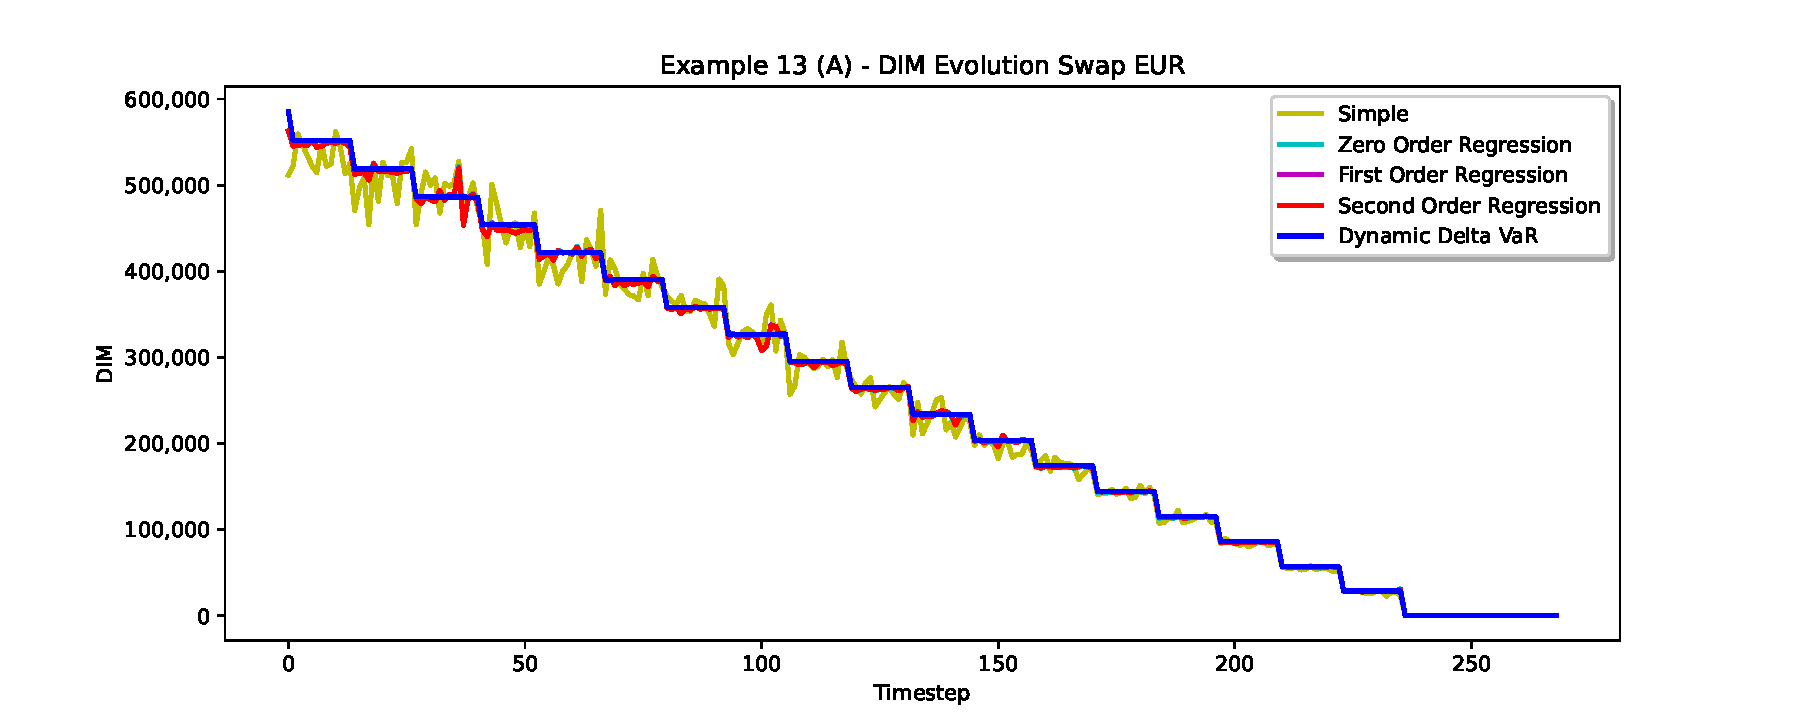
\includegraphics[scale=0.45]{examples/mpl_dim_evolution_A_swap_eur.pdf}
\end{center}
\caption{Evolution of expected Dynamic Initial Margin (DIM) for the EUR Swap of Example 13 A. Regression DIM is evaluated using
  regression of NPV change variances versus the simulated 3M Euribor fixing; regression polynomials are zero, first and
  second order (first and second order curves are not noticebly different in this case). The simulation uses 1000 samples and a time
  grid with bi-weekly steps in line with the Margin Period of Risk.}
\label{fig_ex13a_evolution}
\end{figure}

\begin{figure}[h!]
\begin{center}
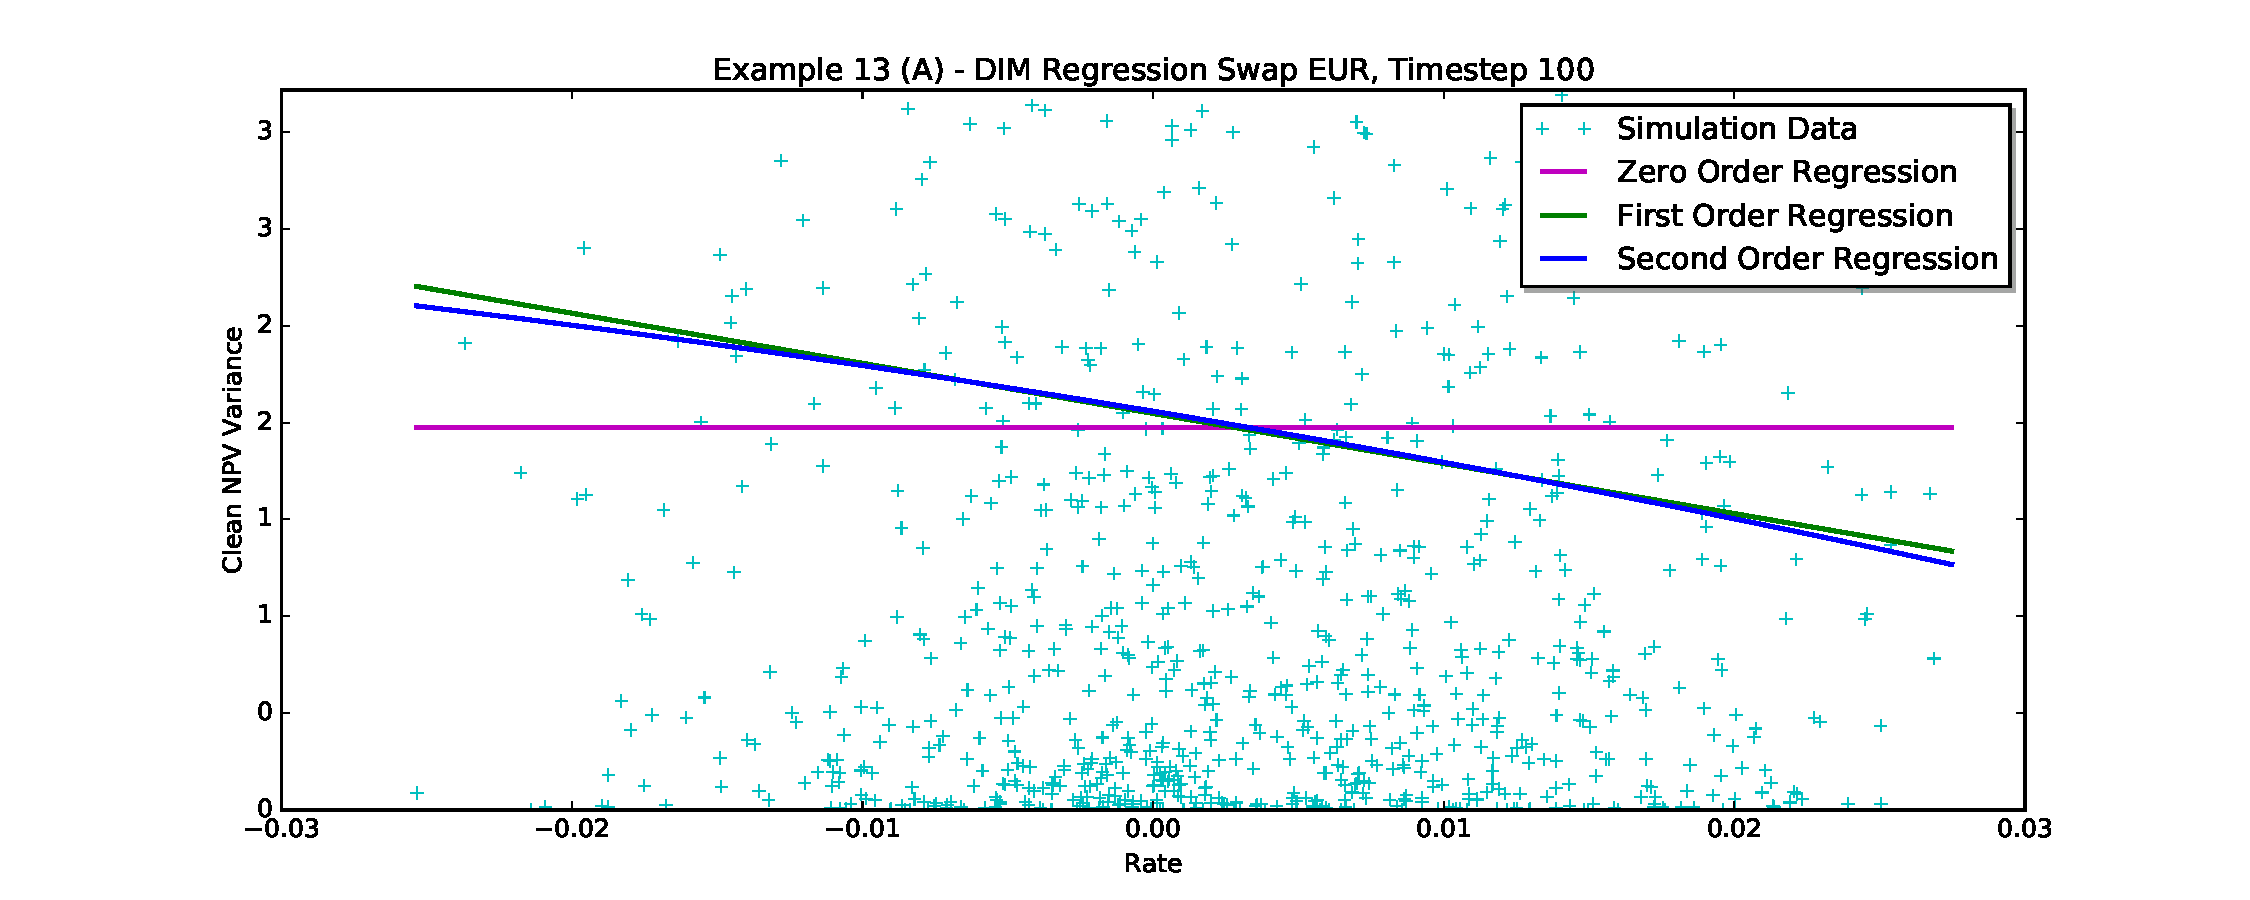
\includegraphics[scale=0.45]{examples/mpl_dim_regression_A_swap_eur.pdf}
\end{center}
\caption{Regression snapshot at time step 100 for the EUR Swap of Example 13 A.}
\label{fig_ex13a_regression}
\end{figure}

The DIM evolution graphs compare a subset of the following Initial Margin projection methods in ORE
\begin{itemize}
\item Simple: 99\% quantile of NPV changes ($\Delta$) over the Margin Period of Risk across all paths, i.e. same IM applied across paths
\item Zero Order ``Regression'': Standard deviation of $\Delta$s scaled to the 99\% quantile with factor 2.33 (normal distribution assumption); same IM applied across paths
\item First/Second Order Regression: Conditional standard deviation of $\Delta$ computed by polynomial first/second order regression of $\Delta$ variances, scaled to the 99\% quantile as avove; different IM amounts applied across paths, graphs show the expected DIM i.e. avergae across paths
\item Dynamic Delta VaR: 99\% quantile VaR based on analytic deltas and vegas computed under scenarios; different IM amounts applied across paths, graphs show the expected DIM i.e. average across paths
\end{itemize}

For a discussion of the regression model performance see \cite{Anfuso2016,LichtersEtAl}. The cases A--E are associated with
various ORE master input files {\tt Input/ore\_A*.xml},  {\tt Input/ore\_B*.xml}, ..., which demonstrate the required simulation
and xva analytic configurations.
 
\begin{figure}[h!]
\begin{center}
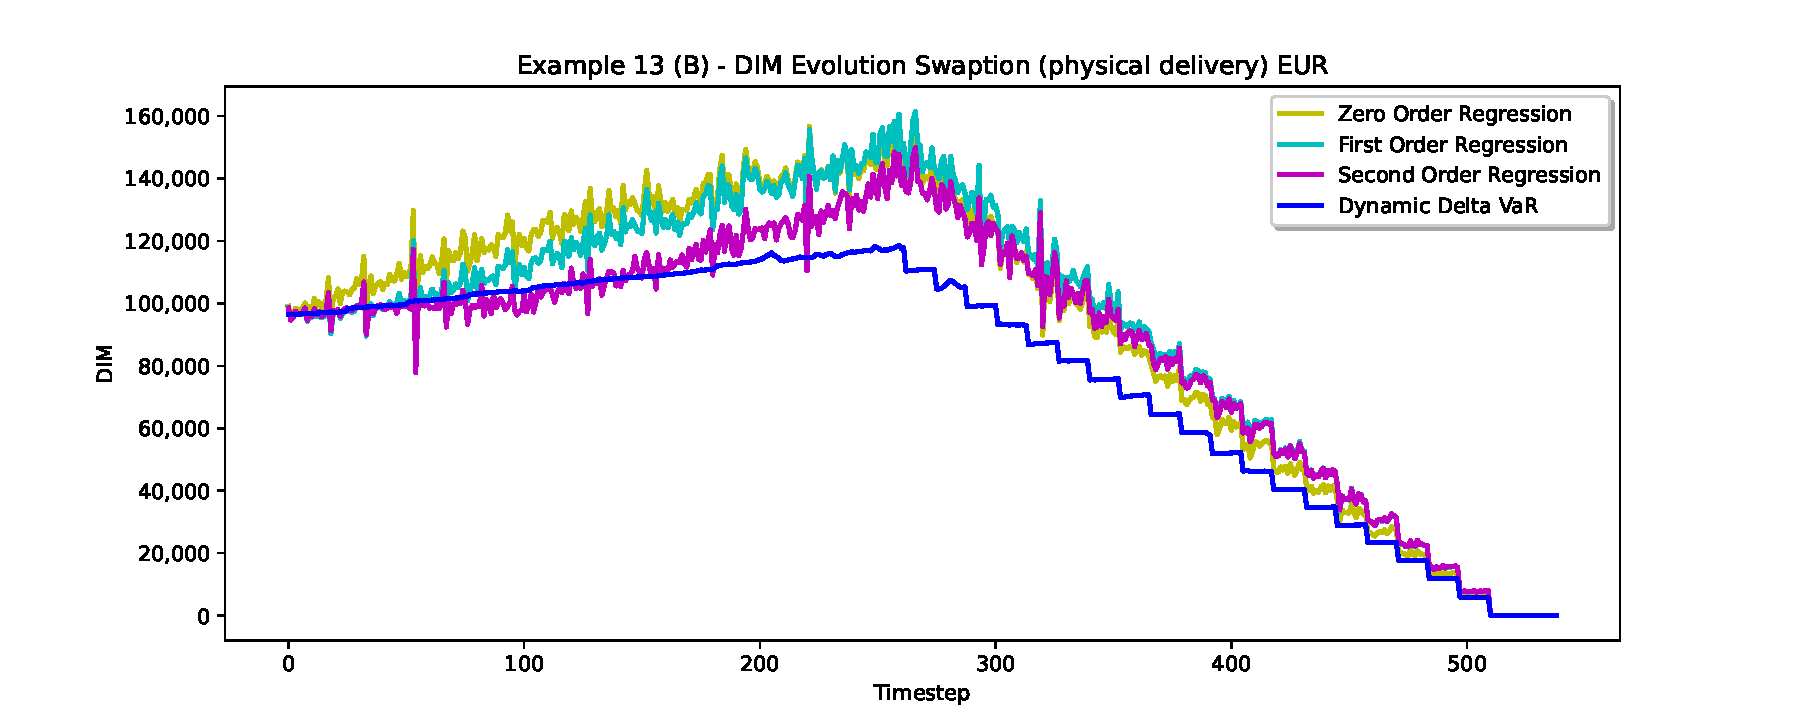
\includegraphics[scale=0.45]{examples/mpl_dim_evolution_B_swaption_eur.pdf}
\end{center}
\caption{Evolution of expected Dynamic Initial Margin (DIM) for the EUR Swaption of Example 13 B with expiry in 10Y
  around time step 100.}
\label{fig_ex13b_evolution}
\end{figure}

\begin{figure}[h!]
\begin{center}
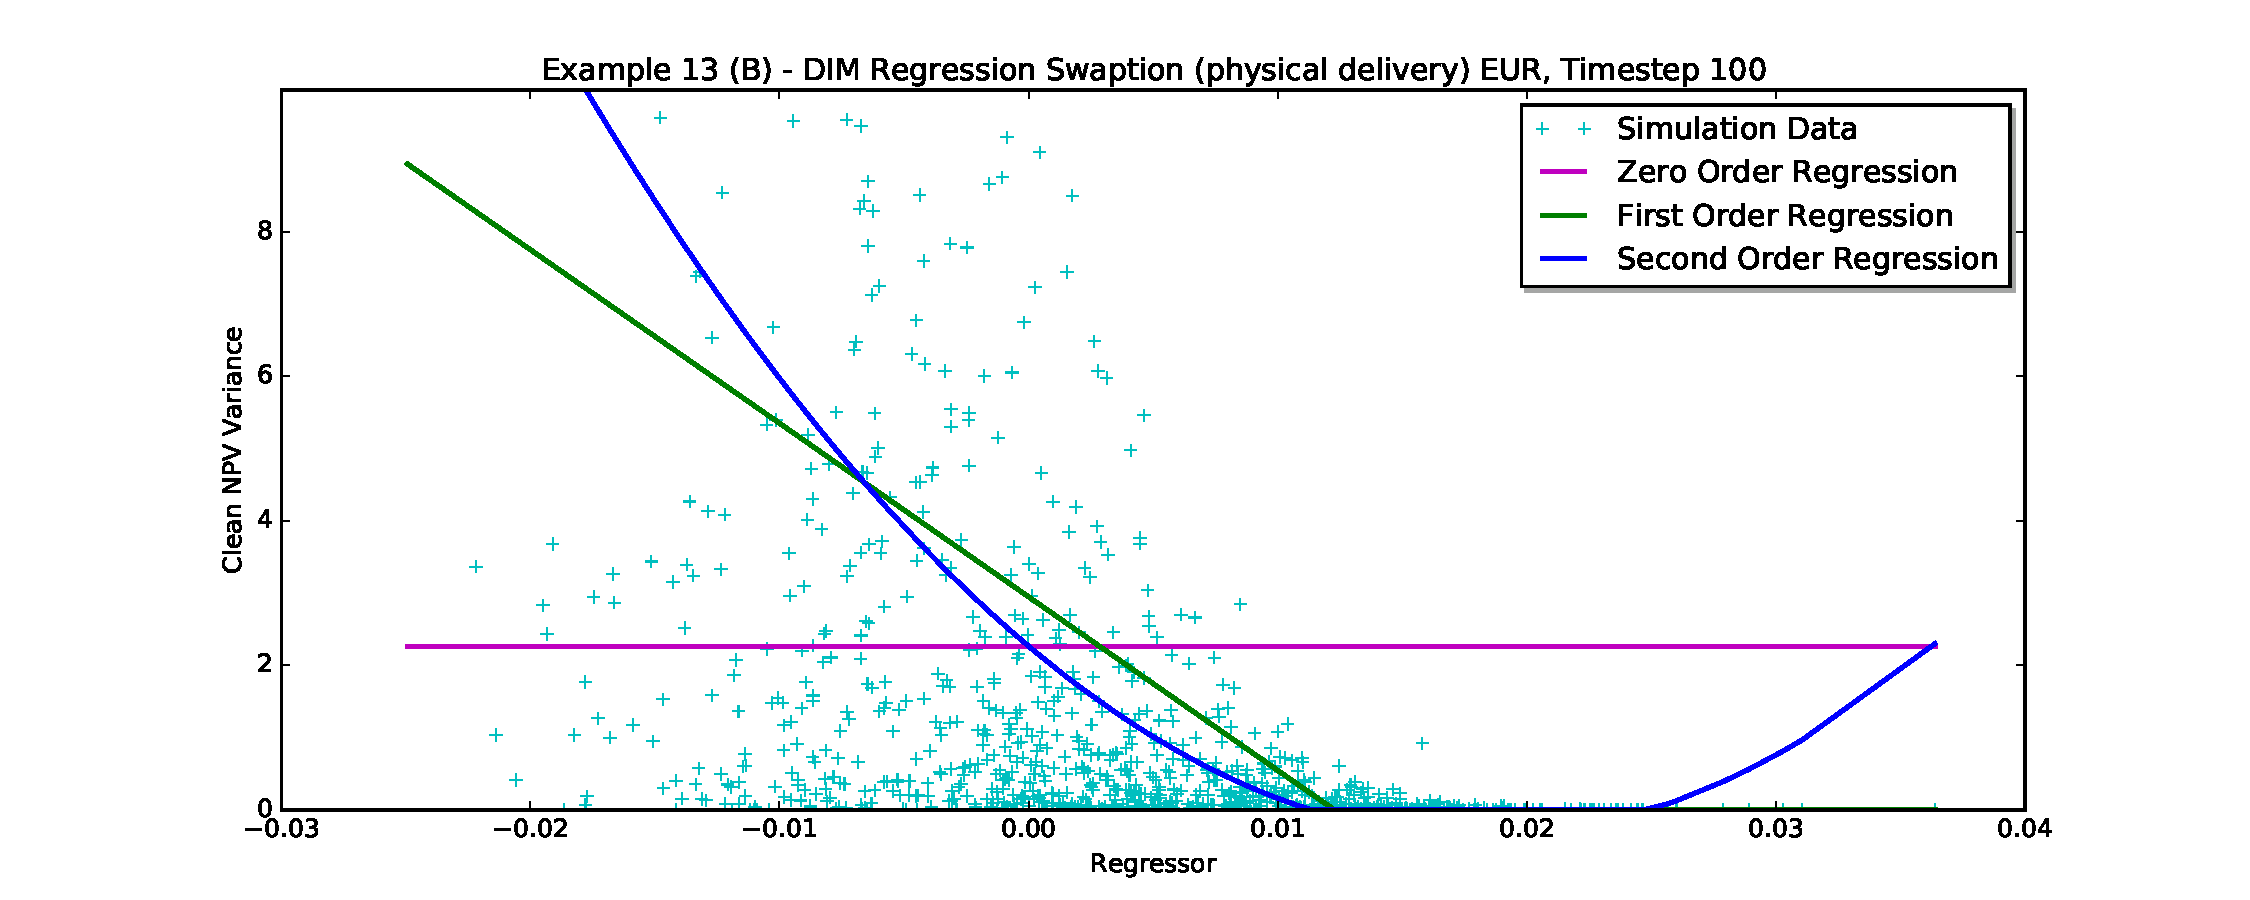
\includegraphics[scale=0.45]{examples/mpl_dim_regression_B_swaption_eur_t100.pdf}
\end{center}
\caption{Regression snapshot at time step 100 (before expiry) for the EUR Swaption of Example 13 B.}
\label{fig_ex13b_regression}
\end{figure}

\begin{figure}[h!]
\begin{center}
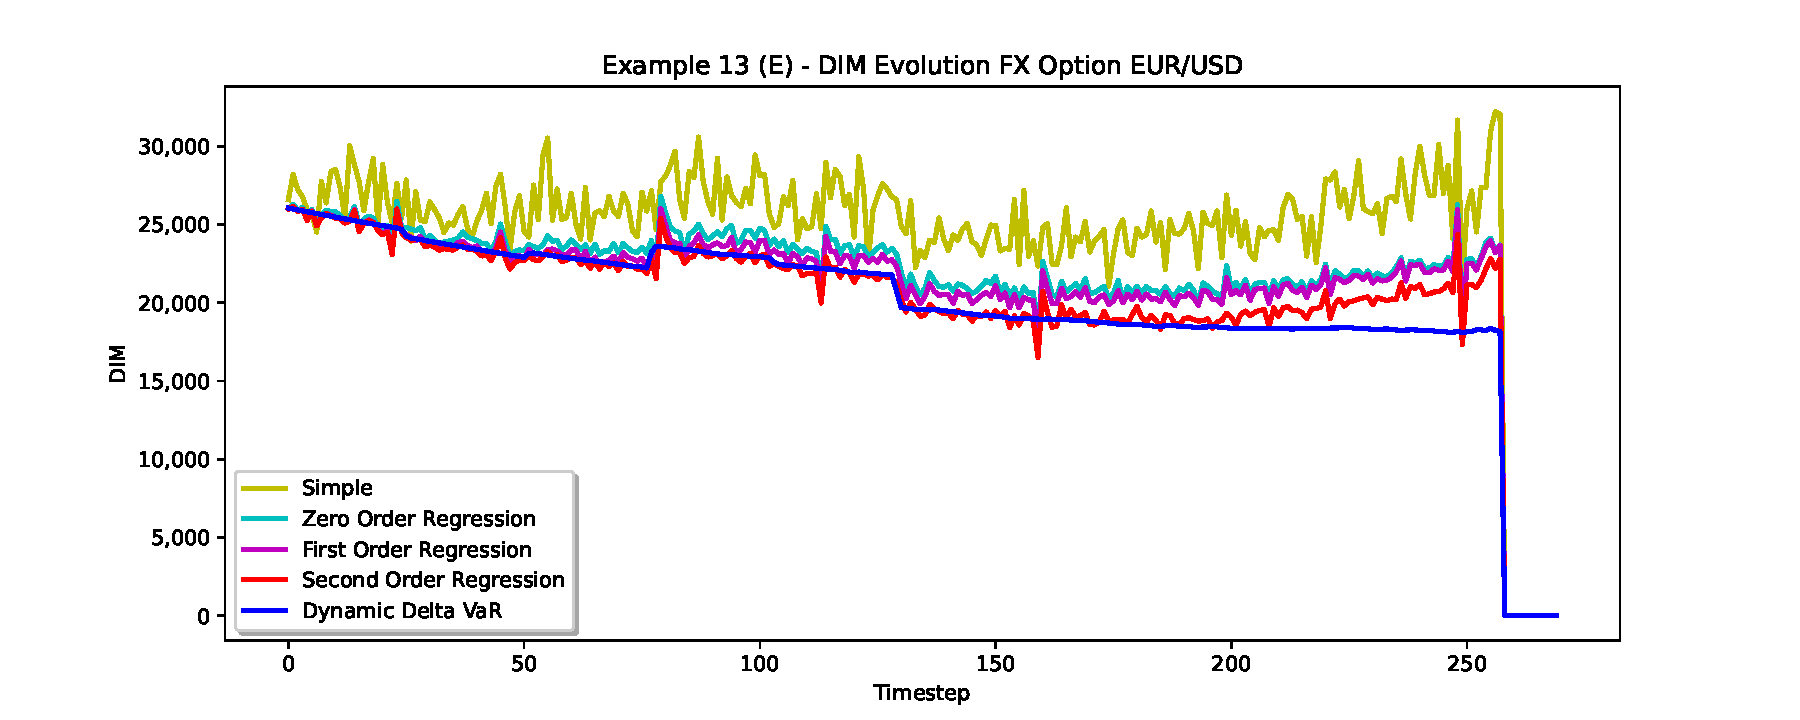
\includegraphics[scale=0.45]{examples/mpl_dim_evolution_E_fxopt.pdf}
\end{center}
\caption{Evolution of expected Dynamic Initial Margin (DIM) for the EUR/USD FX Option of Example 13 (case E) with expiry in 10Y
  around time step 100.}
\label{fig_ex13c_evolution}
\end{figure}

\subsubsection{Dynamic SIMM}

The batch kicked off with ({\tt python run\_dim2.py}) demonstrates a prototype ``Dynamic SIMM'' implementation,
see Input/Dim2/ore\_amccg.xml with
\begin{listing}[H]
%\hrule\medskip
\begin{minted}[fontsize=\footnotesize]{xml}
    <Analytic type="xva">
      ...
      <Parameter name="dimModel">DynamicIM</Parameter>
      ...
    </Analytic>
\end{minted}
\end{listing}
and several related new parameters in the {\tt simulation} section. The new method is embedded into AMC simulation
and uses Algorithmic Differentiation to generate sensitivities along paths which feed into the dynamic SIMM
calculation. Results are -- among others -- a {\tt dim\_evolution.csv} report and a new {\tt dim\_distribution.csv}
report in Output/Dim2/AmcCg.

To validate the new method we apply the ``conventional'' SIMM calculator in ORE that we have enhanced with a CRIF
generator limited to IR/FX risks for this purpose. The {\tt run\_dim2.py} script simulates a few paths, picks one
of the paths and extracts the simulated market data (discount and index curves, FX rates, swaption volatilities)
and writes them to {\tt Input/DimValidation/marketdata.csv}, a market data file in ORE format, and likewise simulated
fixings to {\tt Input/DimValidation/fixings.csv}. The script then loops over simualtion dates of that single path
and performs a conventional SIMM run for each date (see {\tt Input/DimValidation/ore\_simm.xml}).
This is used to check the new method's output on individual paths: When switching off model calibration and setting
model vols close to zero in {\tt Input/Dim2/simulation.xml} and {\tt Input/Dim2/simulation\_amccg.xml}, then we basically
``roll down the forward curve'', and both calculations should yield the same result.
Figure \ref{fig_dim2_comparison_1} shows the comparison and expected outcome.

\begin{figure}[h!]
\begin{center}
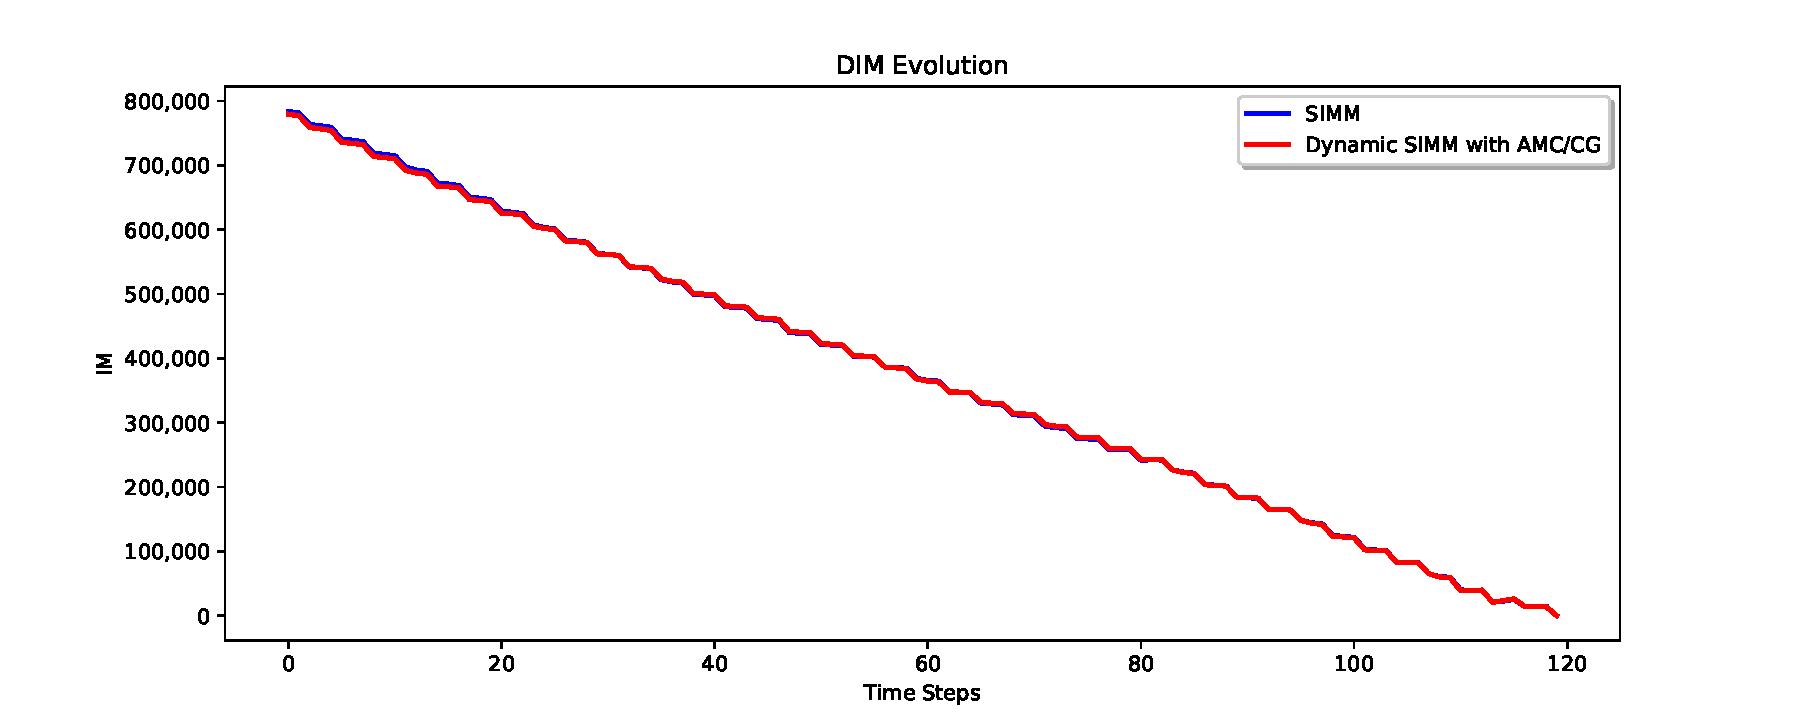
\includegraphics[scale=0.5]{examples/mpl_dim_comparison_1.pdf}
\end{center}
\caption{Evolution of SIMM vs Expected Dynamic Initial Margin (DIM) for a Euribor and SOFR-3M Swap, simulation with zero
  volatility, single path in case of the SIMM benchmark, 10k paths in case of DIM.}
\label{fig_dim2_comparison_1}
\end{figure}

Next, we use a model with non-zero vols, i.e. re-activate calibration in {\tt Input/Dim2/simulation.xml} and
{\tt Input/Dim2/simulation\_amccg.xml}. Running another script ({\tt python run\_dim2\_cube.py}) we now generate a few
SIMM benchmark paths and compare to the expected DIM from 10k paths, see Figure  \ref{fig_dim2_comparison_3}

\begin{figure}[h!]
\begin{center}
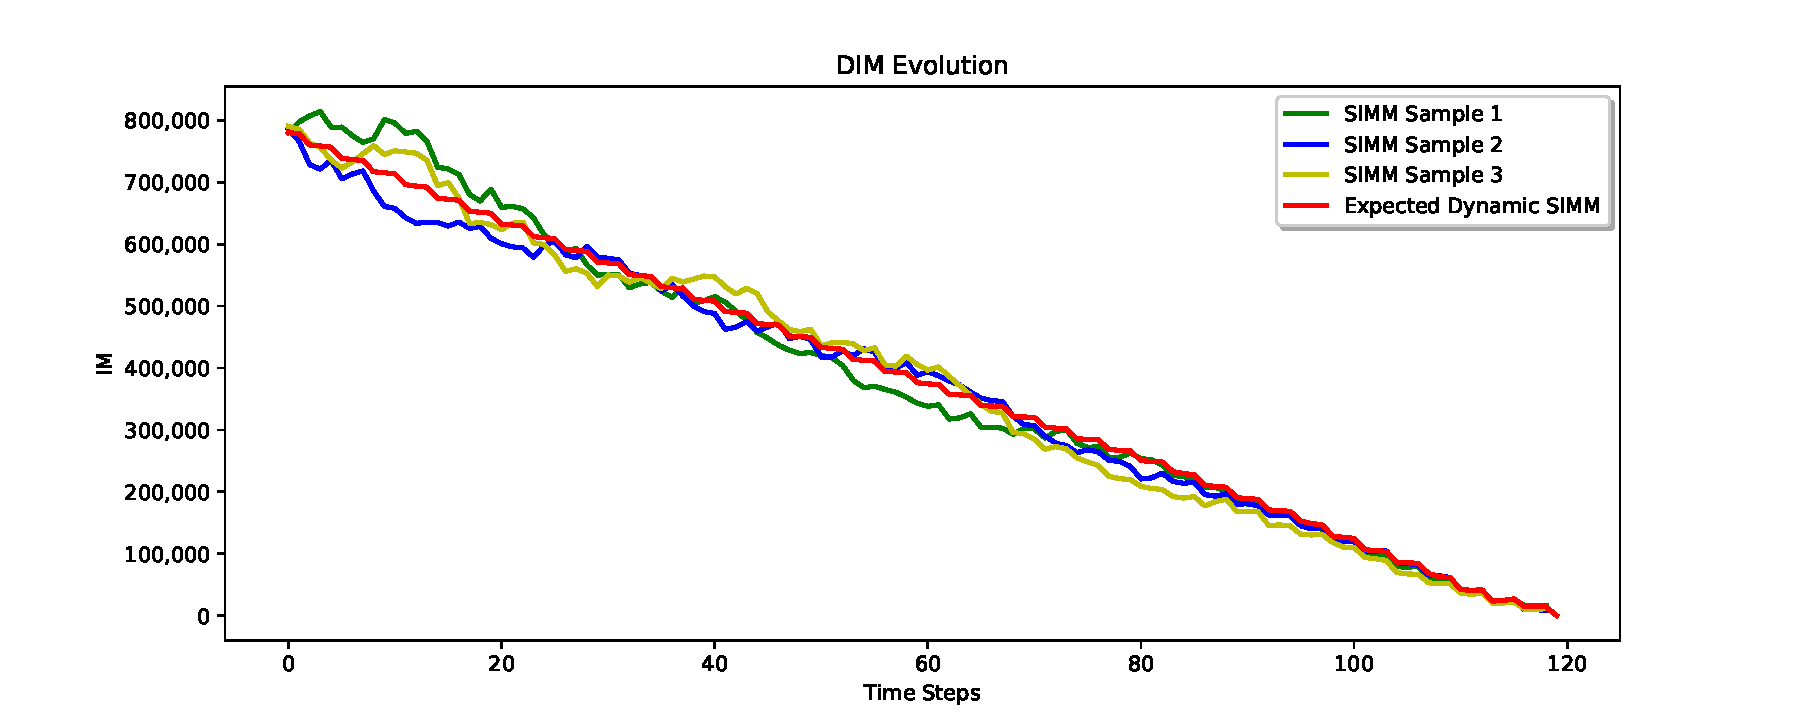
\includegraphics[scale=0.5]{examples/mpl_dim_comparison_3.pdf}
\end{center}
\caption{Evolution of SIMM vs Expected Dynamic Initial Margin (DIM) for a Euribor and SOFR-3M Swap;
  simulation with non-zero volatility, three paths in case of the SIMM benchmark, 10k paths in case of DIM.}
\label{fig_dim2_comparison_3}
\end{figure}

Preliminary note on performance:
\begin{itemize}
\item The script takes about one minute to generate the benchmark SIMM evolution on a single path with 120 time steps
  for the example above
\item Dynamic SIMM takes about 2 minutes for the expectation across 10k paths, on the same hardware (single core, Macbook Pro M2 Max),
  a speedup factor of 5000 compared to the pedestrian benchmark
\end{itemize}

We now zoom in on four future time points (1M, 1Y, 4Y, 8Y) and illustrate the SIMM distribution from the new
report {\tt dim\_distribution.csv}. To benchmark the distributions we re-run {\tt python run\_dim2\_cube.py}
again, but with number of paths increased to 1000 and time steps reduced to the four dates we want to analyse,
i.e. changing Input/Dim2/simulation.xml accordingly. This generates an updated output in Output/DimValidation/simm\_cube.csv.
Running the script {\tt python plot\_dim\_distribution.py} then generates the comparison in Figure
\ref{fig_dim2_distributions}. Note that the Dynamic SIMM calculation takes a few seconds with 10k paths and a handful of time points,
while the brute force benchmark calculation crunches 1k paths on four dates in about half an hour.

\begin{figure}[h!]
\begin{center}
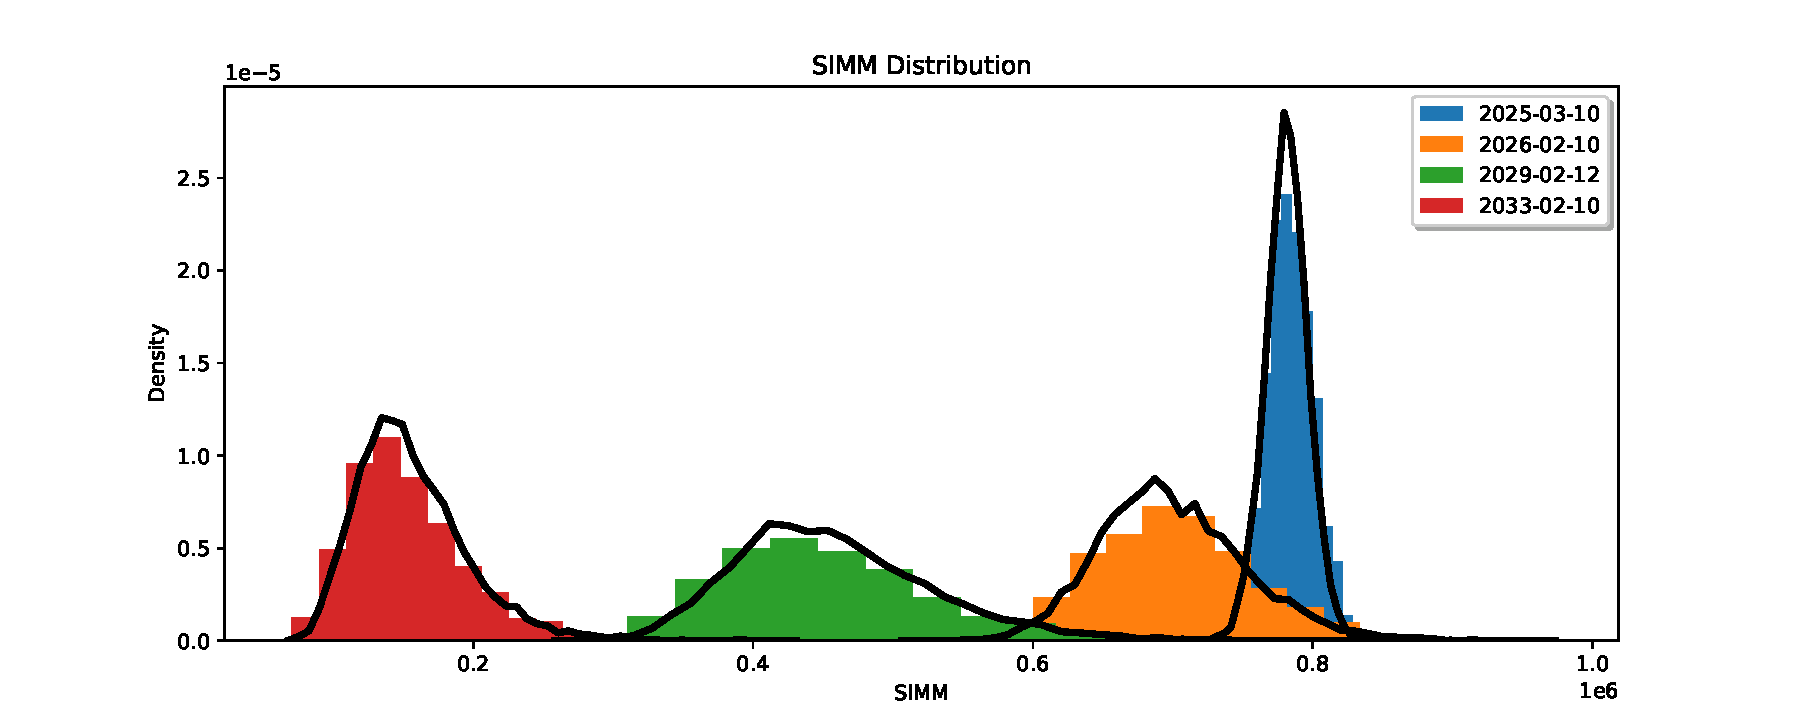
\includegraphics[scale=0.5]{examples/mpl_simm_distribution.pdf}
\end{center}
\caption{SIMM distribution from Dynamic SIMM (lines) vs benchmark (histograms) at time points 1M, 1Y, 4Y, 8Y from as of date.}
\label{fig_dim2_distributions}
\end{figure}

Further investigation of this new Dynamic SIMM method is work in progress:
\begin{itemize}
\item path-wise benchmarking
\item more products - FX Options, Swaptions, FX TaRF as a complex scripted example
\item investigation of alternative regression methods in AMC and their impact on quality of AAD sensitivities
\item comparison to the simple regression DIM model of section \ref{example:initialmargin_dim}
\end{itemize}

\subsection{Exposure}\label{example:exposure}

This section demonstrates exposure simulation and CVA for uncollateralised single trades across ORE's product range, mostly vanilla products.

The examples can be run individually (see below) or all together with {\tt python run.py}.

\begin{itemize}
\item Swap with flat yield curve: {\tt python run\_swapflat.py}
\item Swap with normal yield curves: {\tt python run\_swap.py}
\item FRA: {\tt python run\_fra.py}
\item European/American/Bermudan Swation and CallableSwap: {\tt python run\_swaption.py}
\item Caps/Floors: {\tt python run\_capfloor.py}
\item FX Forward and FX Option: {\tt python run\_fx.py}
\item Resetting and Non-Resetting Cross Currency Swaps: {\tt python run\_ccs.py}
\item Equity Forwards and Option: {\tt python run\_equity.py}
\item Commodity Forward, Option, Swaption, APO: {\tt python run\_commodity.py}
\item Inflation CPI and YOY Swap, the simulation is run twice using a Dodgson-Kainth and Jarrow-Yildirim model: {\tt python run\_inflation.py}
\item Credit Default Swap: {\tt python run\_credit.py}
\end{itemize}

Somewhat more complex single-trade examples:
\begin{itemize}
\item Capped/Floored CMS Spread, Digital CMS Spread: {\tt python run\_cmsspread}
\item Capped CMS Spread and Digital CMS Spread with formula-based payoff (slow): {\tt python run\_fbc.py}
\end{itemize}

Further exposure simulation features:
\begin{itemize}
\item Long-term simulation with and without horizon shift in the Linear Gauss Markov model: {\tt python run\_longterm.py}
\item Simulation in different measures: {\tt python run\_measures.py}
\item Simulation in the two-factor Hull-White model: {\tt python run\_hw2f.py}
\item Wrong-Way-Risk: {\tt python run\_wwr.py}
\item Flip View, switch perspectives easily for XVA: {\tt python run\_flipview.py}
\end{itemize}

All cases are discussed in the following subsections.

\subsubsection{Swap with flat yield curve}\label{example:exposure_swapflat}

We start with a vanilla single currency Swap (currency EUR, maturity 20y, notional 10m, receive fixed 2\% annual, pay
6M-Euribor flat). The market yield curves (for both discounting and forward projection) are set to be flat at 2\% for
all maturities, i.e. the Swap is at the money initially and remains at the money on average throughout its life. Running
ORE in directory {\tt Examples/Exposure} with

\medskip
\centerline{\tt python run\_swapflat.py } 
\medskip

yields the exposure evolution in 

\medskip
\centerline{\tt Examples/swapflat/Output/*.pdf } 
\medskip

and shown in figure \ref{fig_1}. 
\begin{figure}[h!]
\begin{center}
%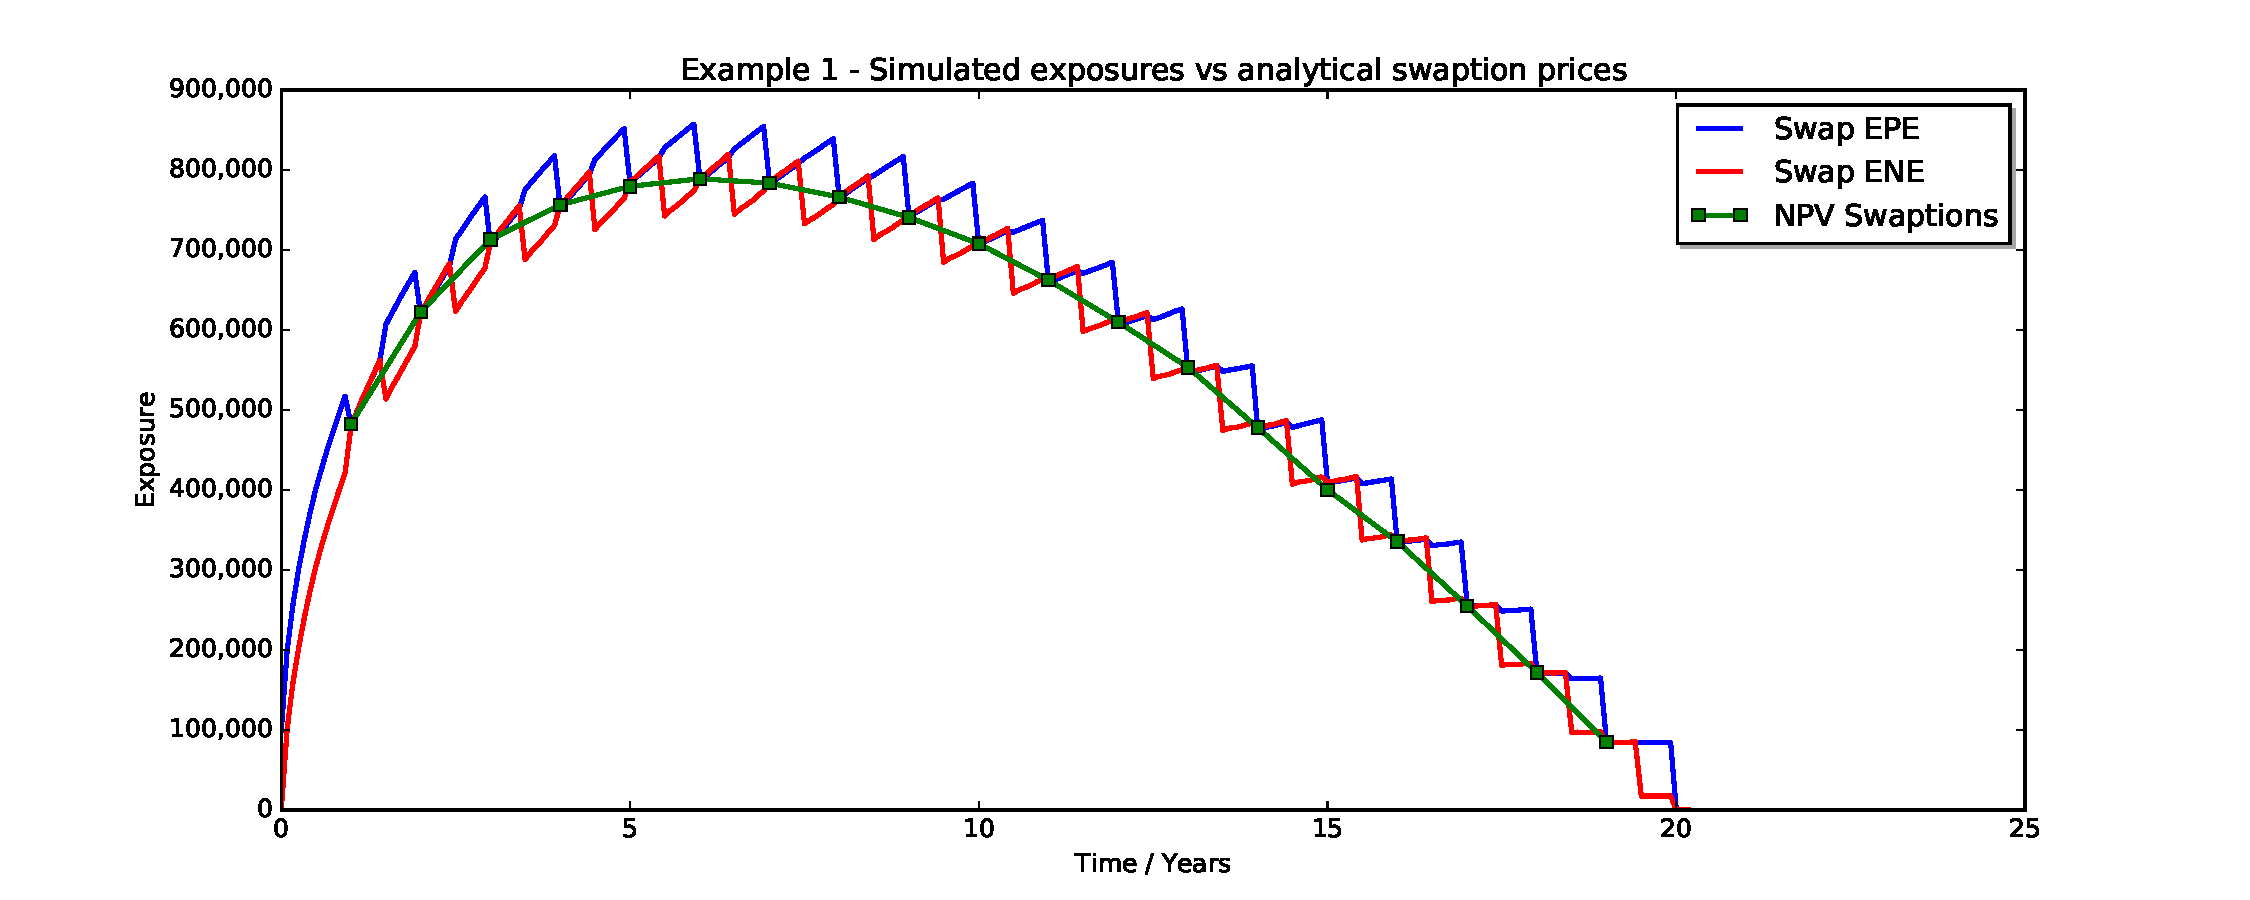
\includegraphics[scale=0.45]{mpl_swap_1_1m_sbb_100k.pdf}
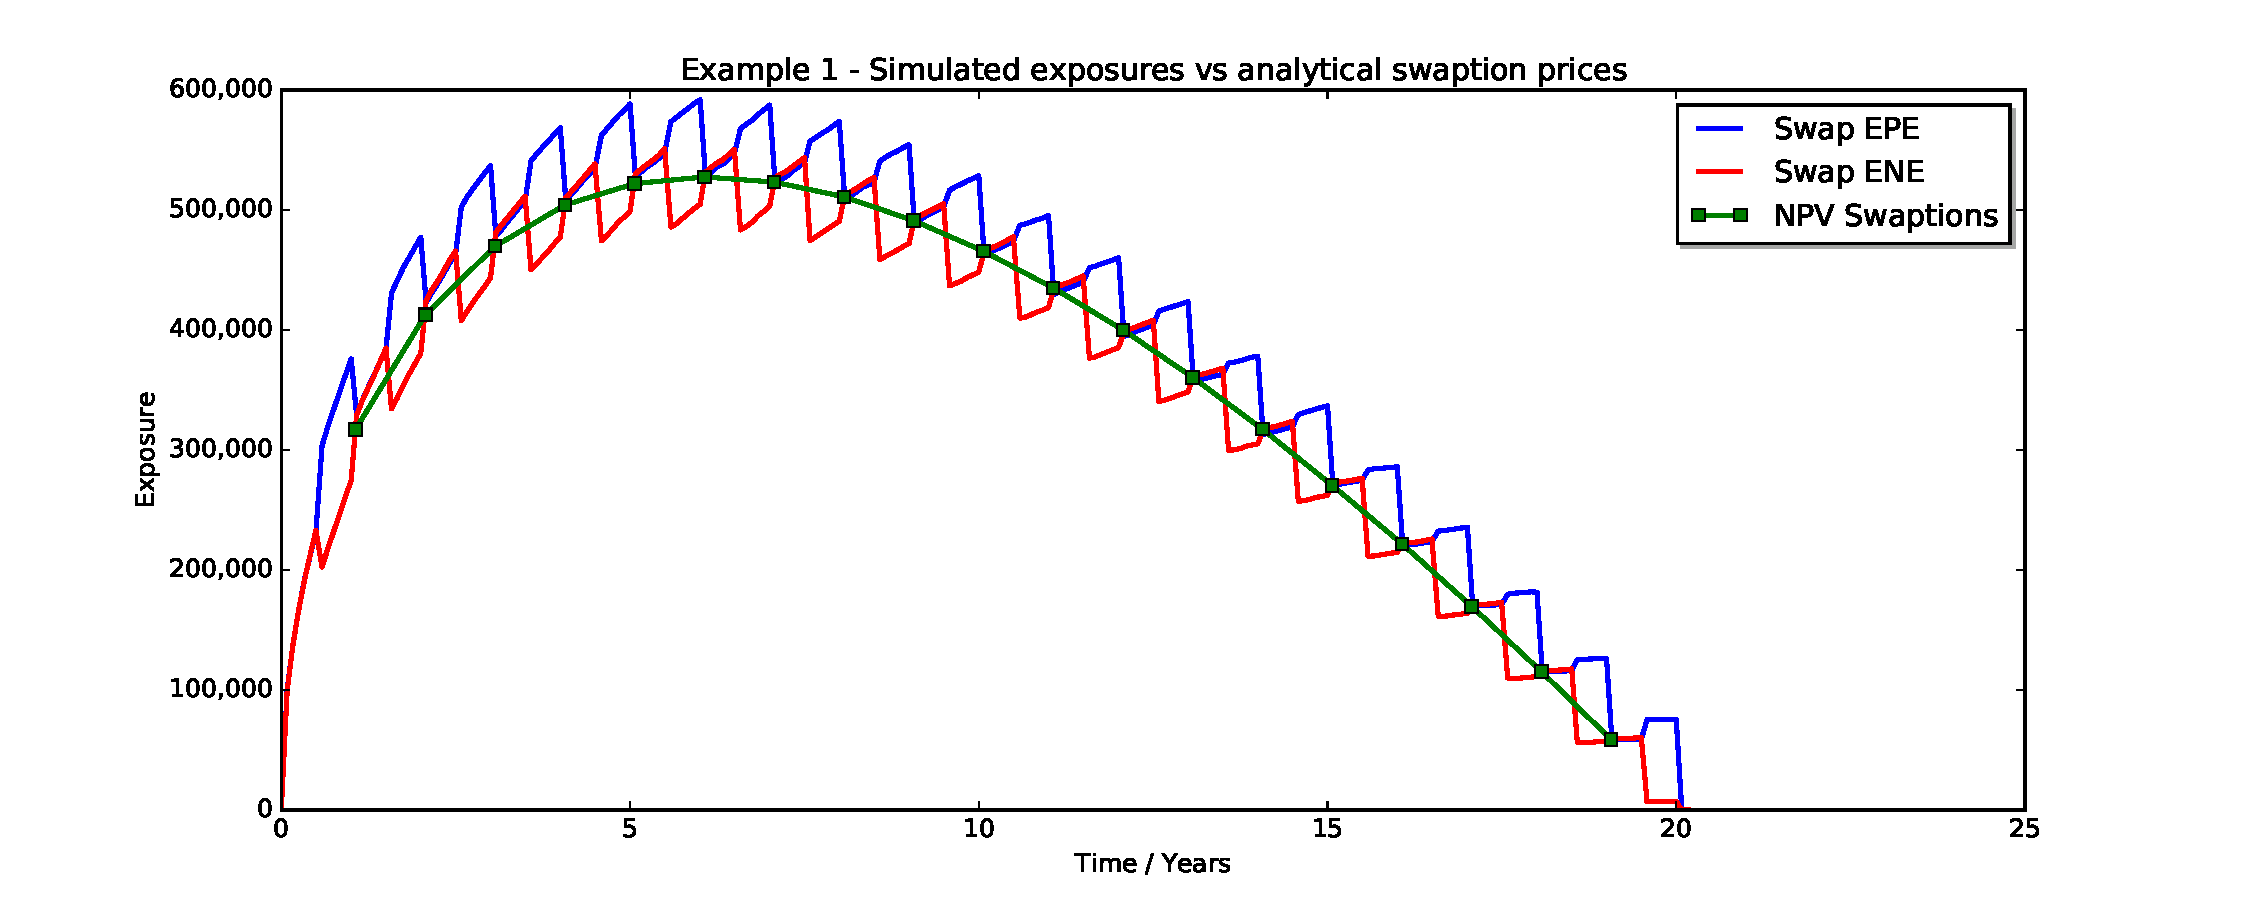
\includegraphics[scale=0.45]{examples/mpl_swap_1_1m_sbb_10k_flat.pdf}
\end{center}
\caption{Vanilla ATM Swap expected exposure in a flat market environment from both parties' perspectives. The symbols are European Swaption prices. The simulation was run with monthly time steps and 10,000 Monte Carlo samples to demonstrate the convergence of EPE and ENE profiles. A similar
outcome can be obtained more quickly with 5,000 samples on a quarterly time grid which is the default setting of Example\_1. }
\label{fig_1}
\end{figure}
Both Swap simulation and Swaption pricing are run with calls to the ORE executable, essentially 

\medskip
\centerline{\tt ore[.exe] ore.xml} 

\centerline{\tt ore[.exe] ore\_swaption.xml} 
\medskip

which are wrapped into the script {\tt Examples/Exposure/run\_swapflat.py} provided with the ORE release.
It is instructive to look into the input folder in Examples/Exposure/Output/swapflat, the content of the main input file {\tt
  ore.xml}, together with the explanations in section \ref{sec:configuration}. \\

This simple example is an important test case which is also run similarly in one of the unit test suites of ORE. The
expected exposure can be seen as a European option on the underlying netting set, see also \cite{methods}.
In this example, the expected exposure at some future point in time, say 10 years, is equal to
the European Swaption price for an option with expiry in 10 years, underlying Swap start in 10 years and underlying Swap
maturity in 20 years. We can easily compute such standard European Swaption prices for all future points in time where
both Swap legs reset, i.e. annually in this case\footnote{Using closed form expressions for standard European Swaption
  prices.}. And if the simulation model has been calibrated to the points on the Swaption surface which are used for
European Swaption pricing, then we can expect to see that the simulated exposure matches Swaption prices at these annual
points, as in figure \ref{fig_1}.  In Example\_1 we used co-terminal ATM Swaptions for both model calibration and
Swaption pricing. Moreover, as the yield curve is flat in this example, the exposures from both parties'
perspectives (EPE and ENE) match not only at the annual resets, but also for the period between annual reset of both
legs to the point in time when the floating leg resets. Thereafter, between floating leg (only) reset and next joint
fixed/floating leg reset, we see and expect a deviation of the two exposure profiles.

\subsubsection{Swap with normal yield curves}\label{example:exposure_swap}

Moving to the next case we see what changes when using a realistic (non-flat) market
environment. Running the example with

\medskip
\centerline{\tt python run\_swap.py } 
\medskip

yields the exposure evolution in 

\medskip
\centerline{\tt Examples/Exposure/Output/swap/*.pdf } 
\medskip

shown in figure \ref{fig_2}.
\begin{figure}[h!]
\begin{center}
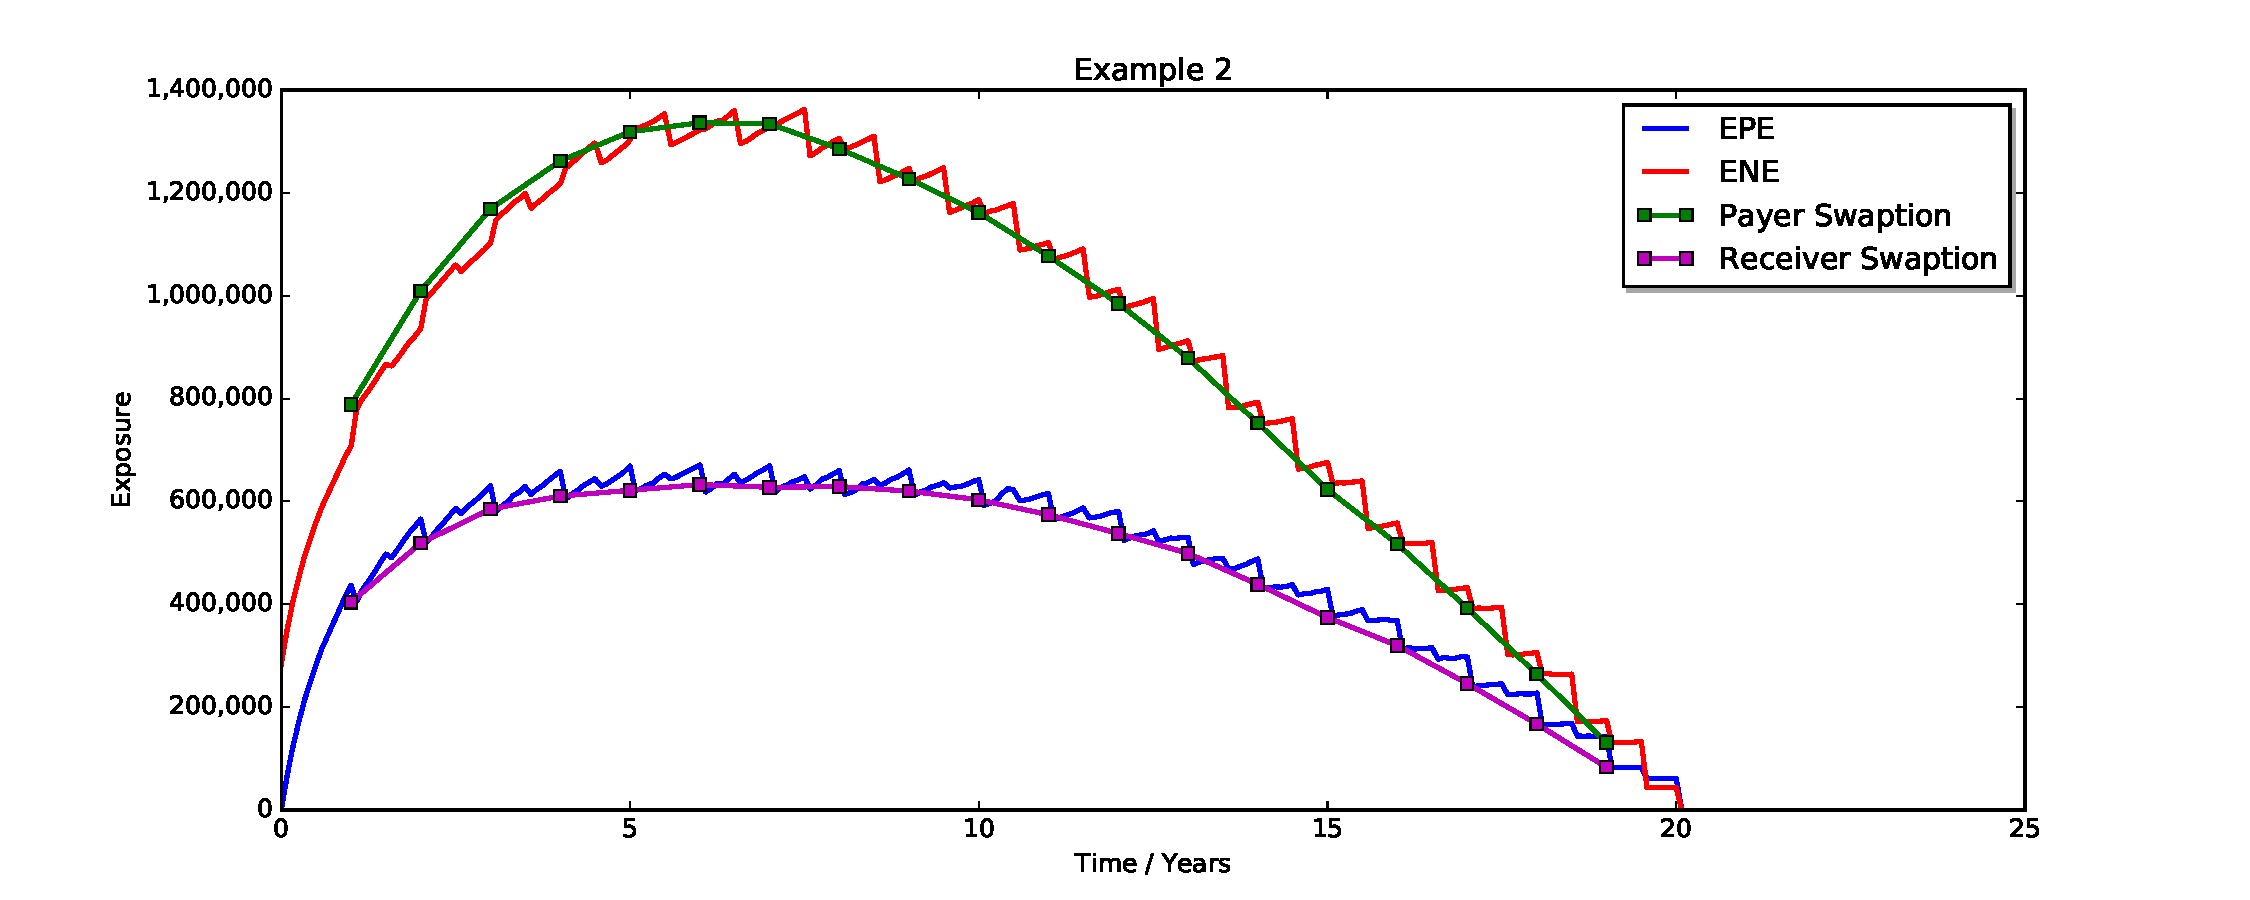
\includegraphics[scale=0.45]{examples/mpl_swap_3.pdf}
\end{center}
\caption{Vanilla ATM Swap expected exposure in a realistic market environment as of 05/02/2016 from both parties'
  perspectives. The Swap is the same as in figure \ref{fig_1} but receiving fixed 1\%, roughly at the money. The symbols
  are the prices of European payer and receiver Swaptions. Simulation with 5000 paths and monthly time steps.}
\label{fig_2}
\end{figure}
In this case, where the curves (discount and forward) are upward sloping, the receiver Swap is at the money at inception
only and moves (on average) out of the money during its life. Similarly, the Swap moves into the money from the
counterparty's perspective. Hence the expected exposure evolutions from our perspective (EPE) and the counterparty's
perspective (ENE) 'detach' here, while both can still be be reconciled with payer or respectively receiver Swaption
prices.

\subsubsection{Forward Rate Agreement}\label{example:exposure_fra}

The example in {\tt run\_fra.py} demonstrates pricing, cash flow projection and exposure simulation for two additional products
\begin{itemize}
\item Forward Rate Agreements
\item Averaging Overnight Index Swaps
\end{itemize}
using a minimal portfolio of four trades, one FRA and three OIS. The essential results are in {\tt npv.csv}, {\tt flows.csv} and 
four {\tt exposure\_trade\_*.csv} files in folder {\tt Examples/Exposure/Output/fra}.

\subsubsection{Swaptions}\label{example:exposure_swaptions}

The batch in {\tt python run\_swaption.py} covers three cases
\begin{itemize}
\item European Swaptions with cash and physical settlement, compared to the underlying Forward Swap, see figure \ref{fig_3}:\\
  The delivery type (cash vs physical) yields significantly different valuations as of today due to the steepness of the
  relevant yield curves (EUR). The cash settled Swaption's exposure graph is truncated at the exercise date, whereas the
  physically settled Swaption exposure turns into a Swap-like exposure after expiry. For comparison, the example also
  provides the exposure evolution of the underlying forward starting Swap which yields a somewhat higher exposure after
  the forward start date than the physically settled Swaption. This is due to scenarios with negative Swap NPV at expiry
  (hence not exercised) and positive NPVs thereafter. Note the reduced EPE in case of a Swaption with settlement of the
  option premium on exercise date.
\item Bermudan and American Swaption, see figure \ref{fig_3b}: \\
  The underlying Swap is the same as in the European Swaption example above. Note in
  particular the difference between the Bermudan and European Swaption exposures with cash settlement: The Bermudan shows
  the typical step-wise decrease due to the series of exercise dates. Also note that we are using the same Bermudan option
  pricing engines for both settlement types, in contrast to the European case, so that the Bermudan option cash and
  physical exposures are identical up to the first exercise date. When running this example, you will notice the
  significant difference in computation time compared to the European case (ballpark 30 minutes here for 2 Swaptions, 1000
  samples, 90 time steps). The Bermudan example takes significantly more computation time because we use an LGM grid
  engine for pricing under scenarios in this case. In a realistic context one would more likely resort to American Monte
  Carlo simulation, feasible in ORE, but not provided in the current release. However, this implementation can be used to
  benchmark any faster / more sophisticated approach to Bermudan Swaption exposure simulation.
\item European Callable Swap, represented as two trades -- the non-callable Swap and a Swaption
  with physical delivery. We have sold the call option, i.e. the Swaption is a right for the counterparty to enter into
  an offsetting Swap which economically terminates all future flows if exercised. The resulting exposure evolutions
  for the individual components (Swap, Swaption), as well as the callable Swap are shown in figure \ref{fig_4}.
  The example is an extreme case where the underlying Swap is deeply in the money (receiving fixed 5\%), and hence the
  call exercise probability is close to one. Modify the Swap and Swaption fixed rates closer to the money ($\approx$ 1\%)
  to see the deviation between net exposure of the callable Swap and the exposure of a 'short' Swap with maturity on
  exercise. We have added more recently the combined CallableSwap instrument representation, check {\tt portfolio.xml}
  and compare the CallableSwap NPV in {\tt npv.csv} to the package NPV of Swap and Swaption.
\end{itemize}

\begin{figure}[htb]
\begin{center}
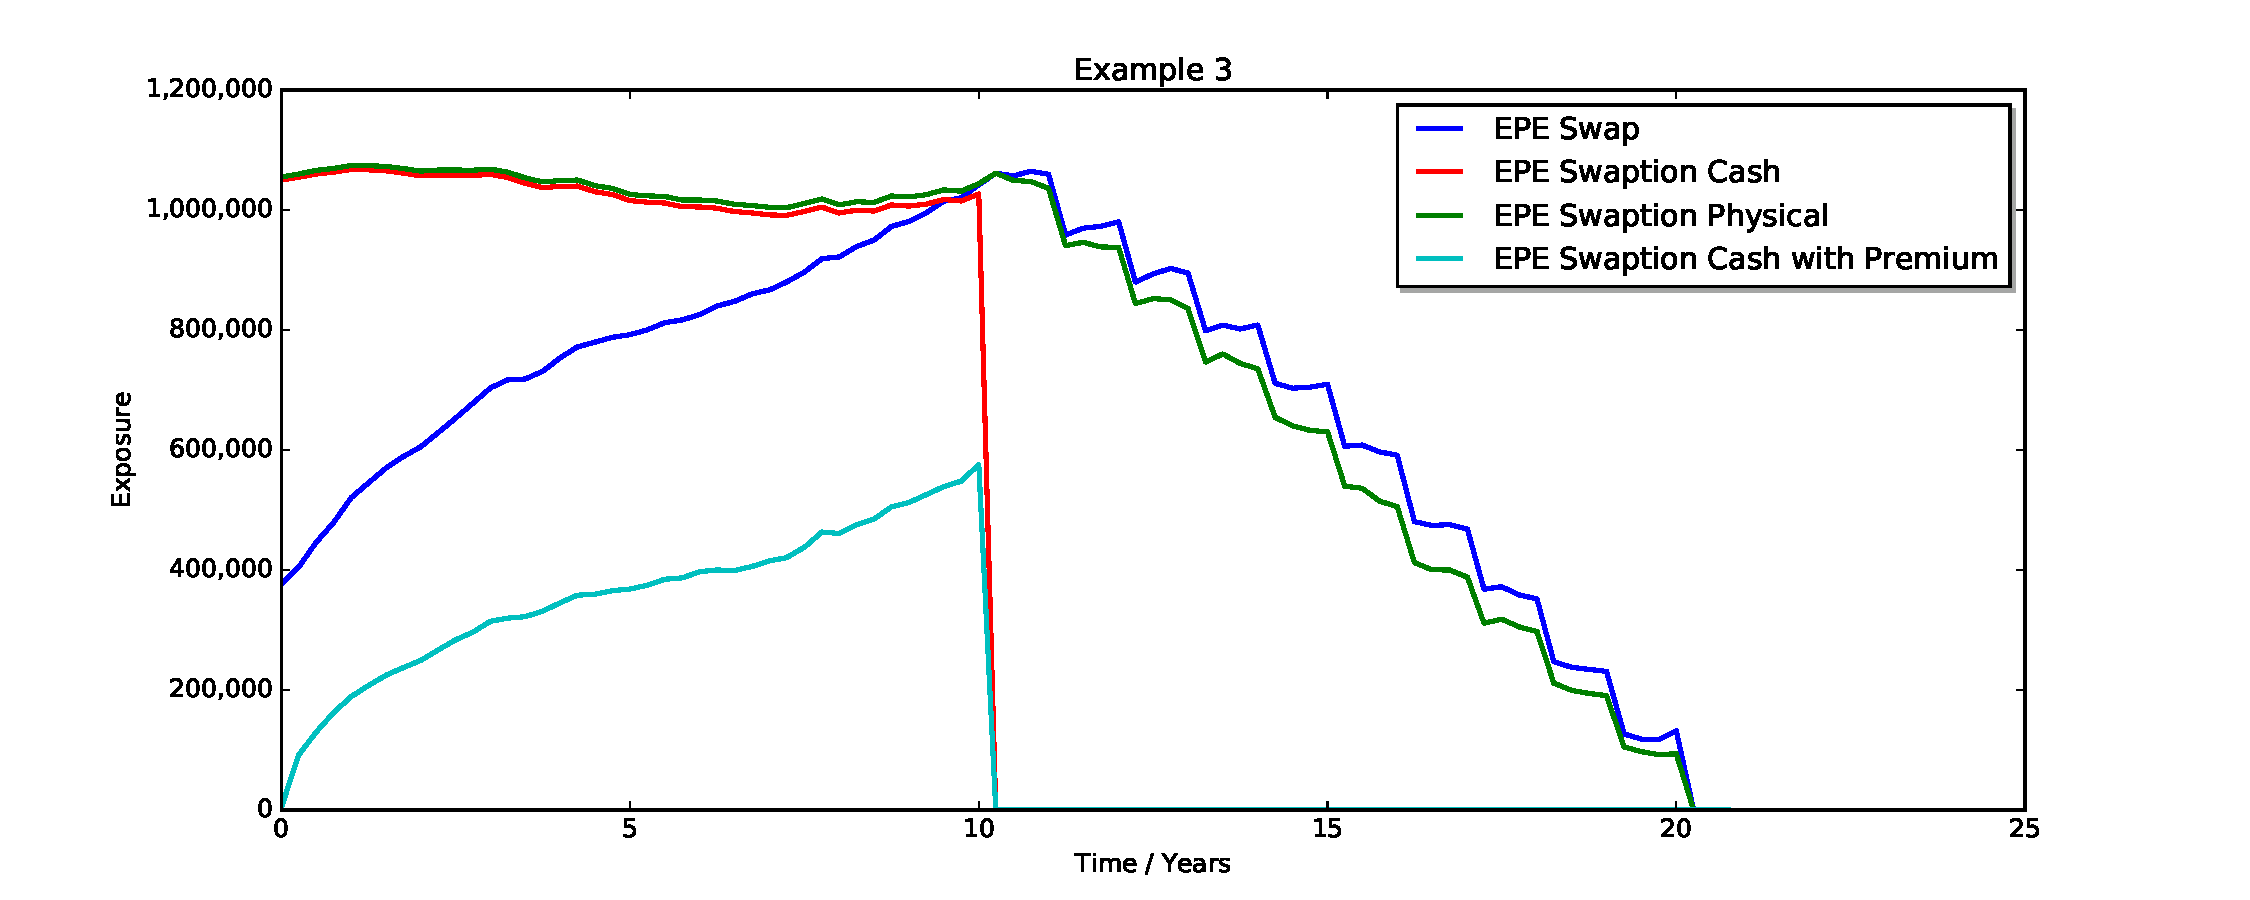
\includegraphics[scale=0.45]{examples/mpl_swaption.pdf}
\end{center}
\caption{European Swaption exposure evolution, expiry in 10 years, final maturity in 20 years, for cash and physical
  delivery. Simulation with 1000 paths and quarterly time steps. }
\label{fig_3}
\end{figure}

\begin{figure}[htb]
\begin{center}
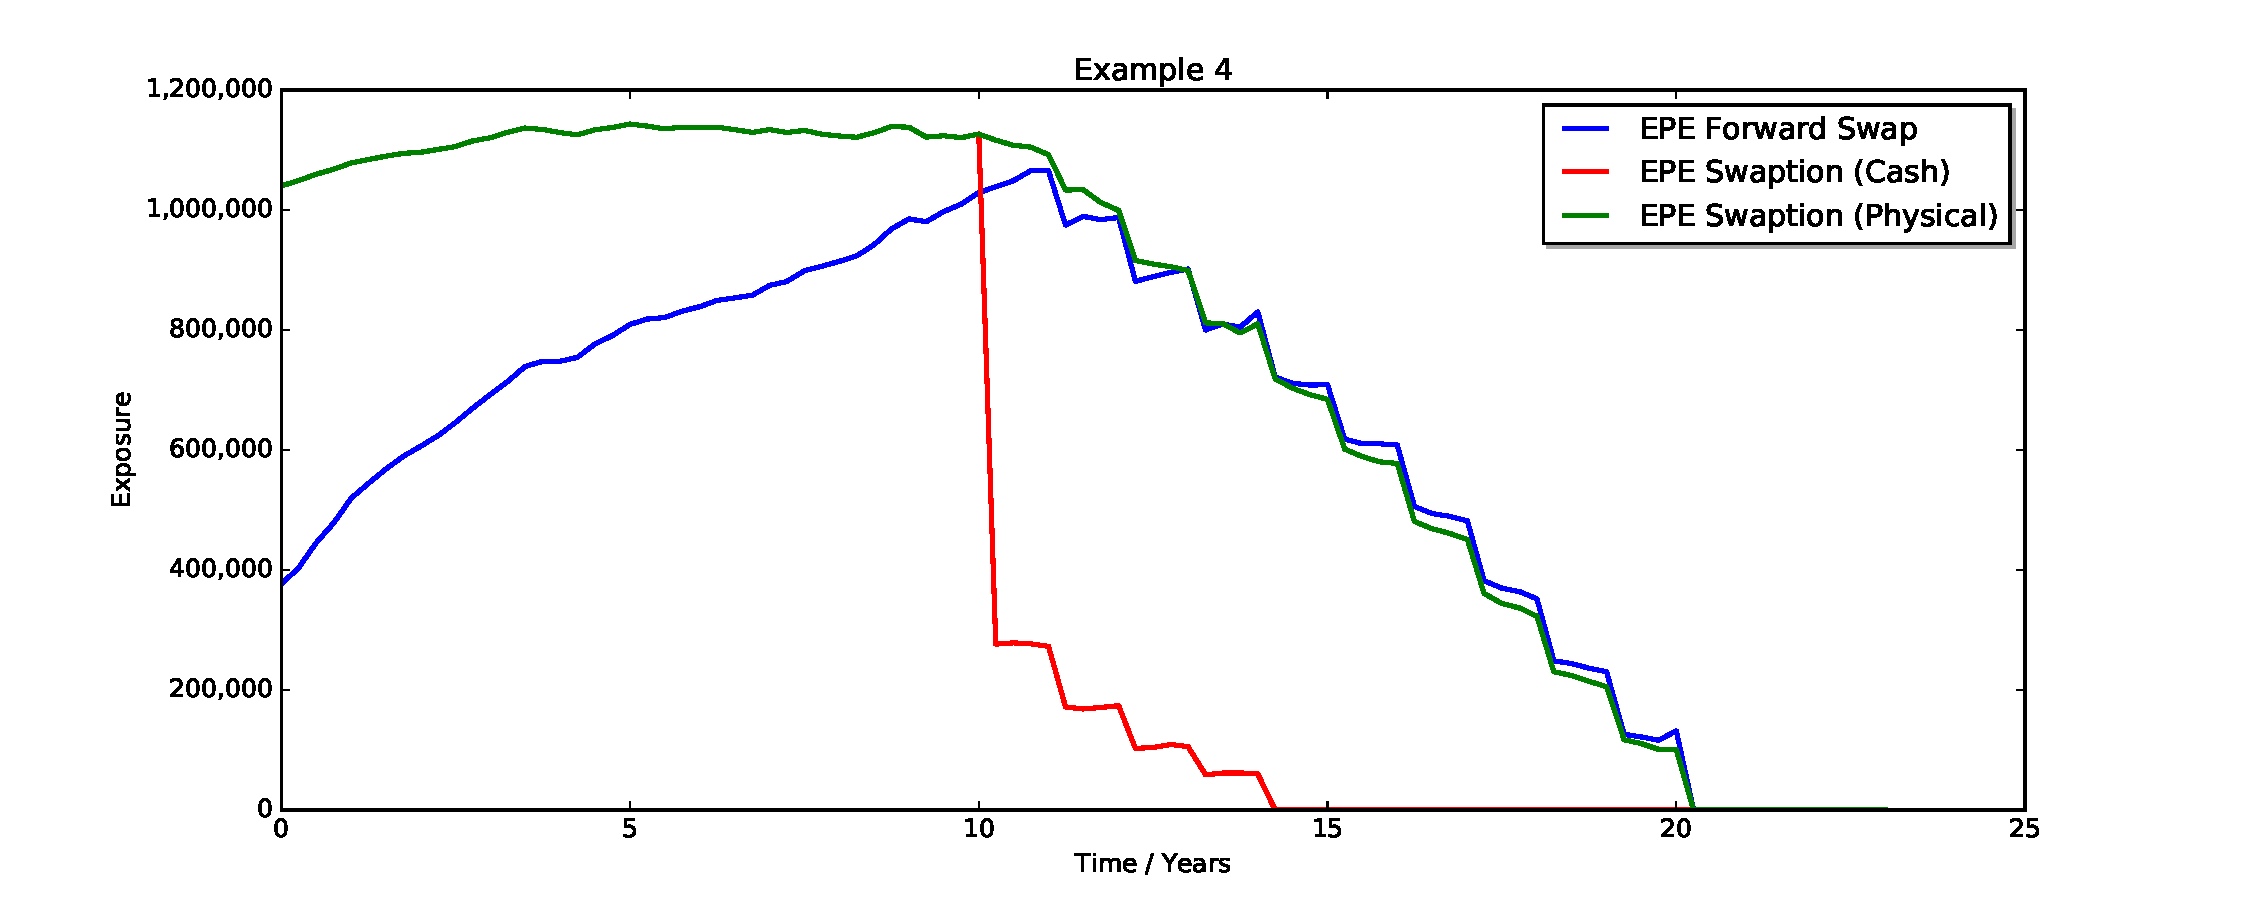
\includegraphics[scale=0.45]{examples/mpl_bermudan_swaption.pdf}
\end{center}
\caption{Bermudan Swaption exposure evolution, 5 annual exercise dates starting in 10 years, final maturity in 20 years,
  for cash and physical delivery. Simulation with 1000 paths and quarterly time steps.}
\label{fig_3b}
\end{figure}

\begin{figure}[hbt]
\begin{center}
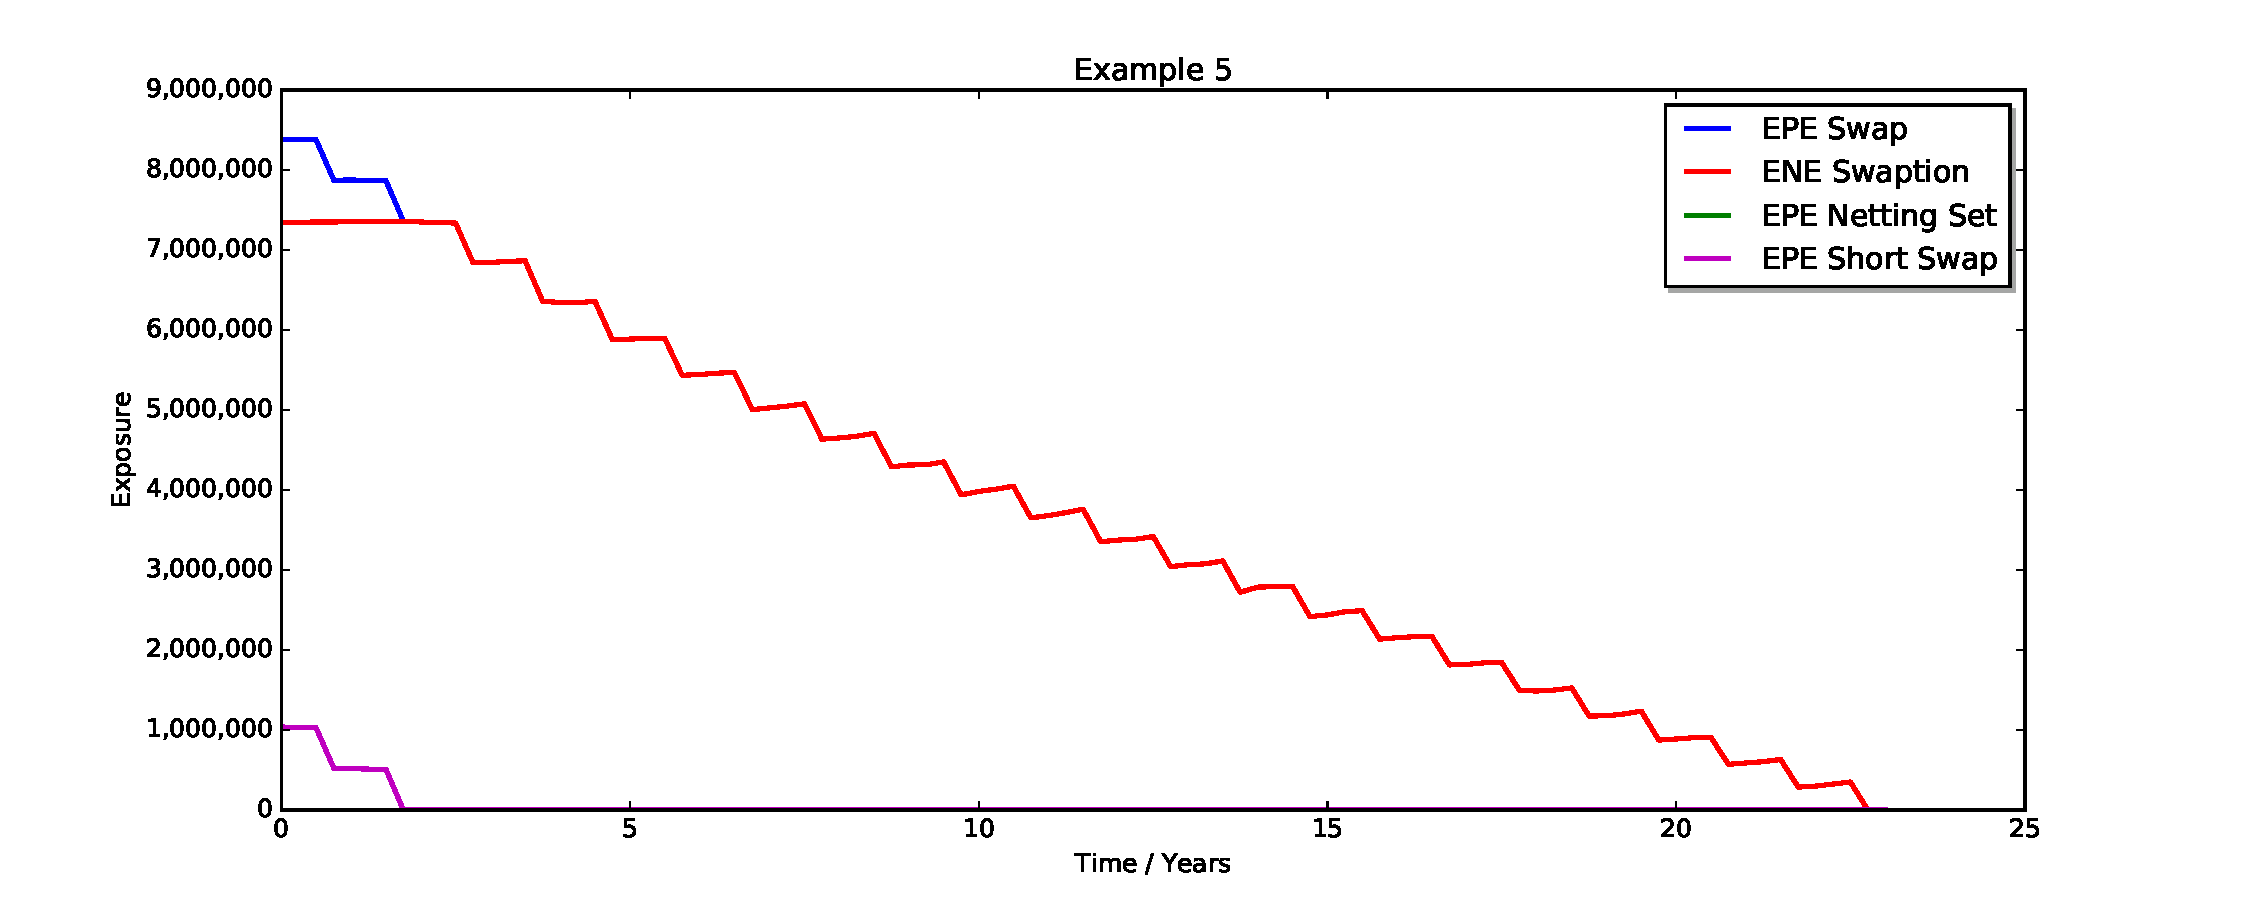
\includegraphics[scale=0.45]{examples/mpl_callable_swap.pdf}
\end{center}
\caption{European callable Swap represented as a package consisting of non-callable Swap and Swaption. The Swaption has
  physical delivery and offsets all future Swap cash flows if exercised. The exposure evolution of the package is shown
  here as 'EPE Netting Set' (green line). This is covered by the pink line, the exposure evolution of the same Swap but
  with maturity on the exercise date. The graphs match perfectly here, because the example Swap is deep in the money and
  exercise probability is close to one. Simulation with 5000 paths and quarterly time steps.}
\label{fig_4}
\end{figure}

\clearpage

\subsubsection{Cap/Floor}\label{example:exposure_capfloor}

The example {\tt python run\_capfloor.py} generates exposure evolutions of several Swaps, Caps and Floors. The
example shown in figure \ref{fig_capfloor_1} ('portfolio 1') consists of a 20y Swap receiving 3\% fixed and paying
Euribor 6M plus a long 20y Collar with both cap and floor at 4\% so that the net exposure corresponds to a Swap
paying 1\% fixed. \\

\begin{figure}[h!]
\begin{center}
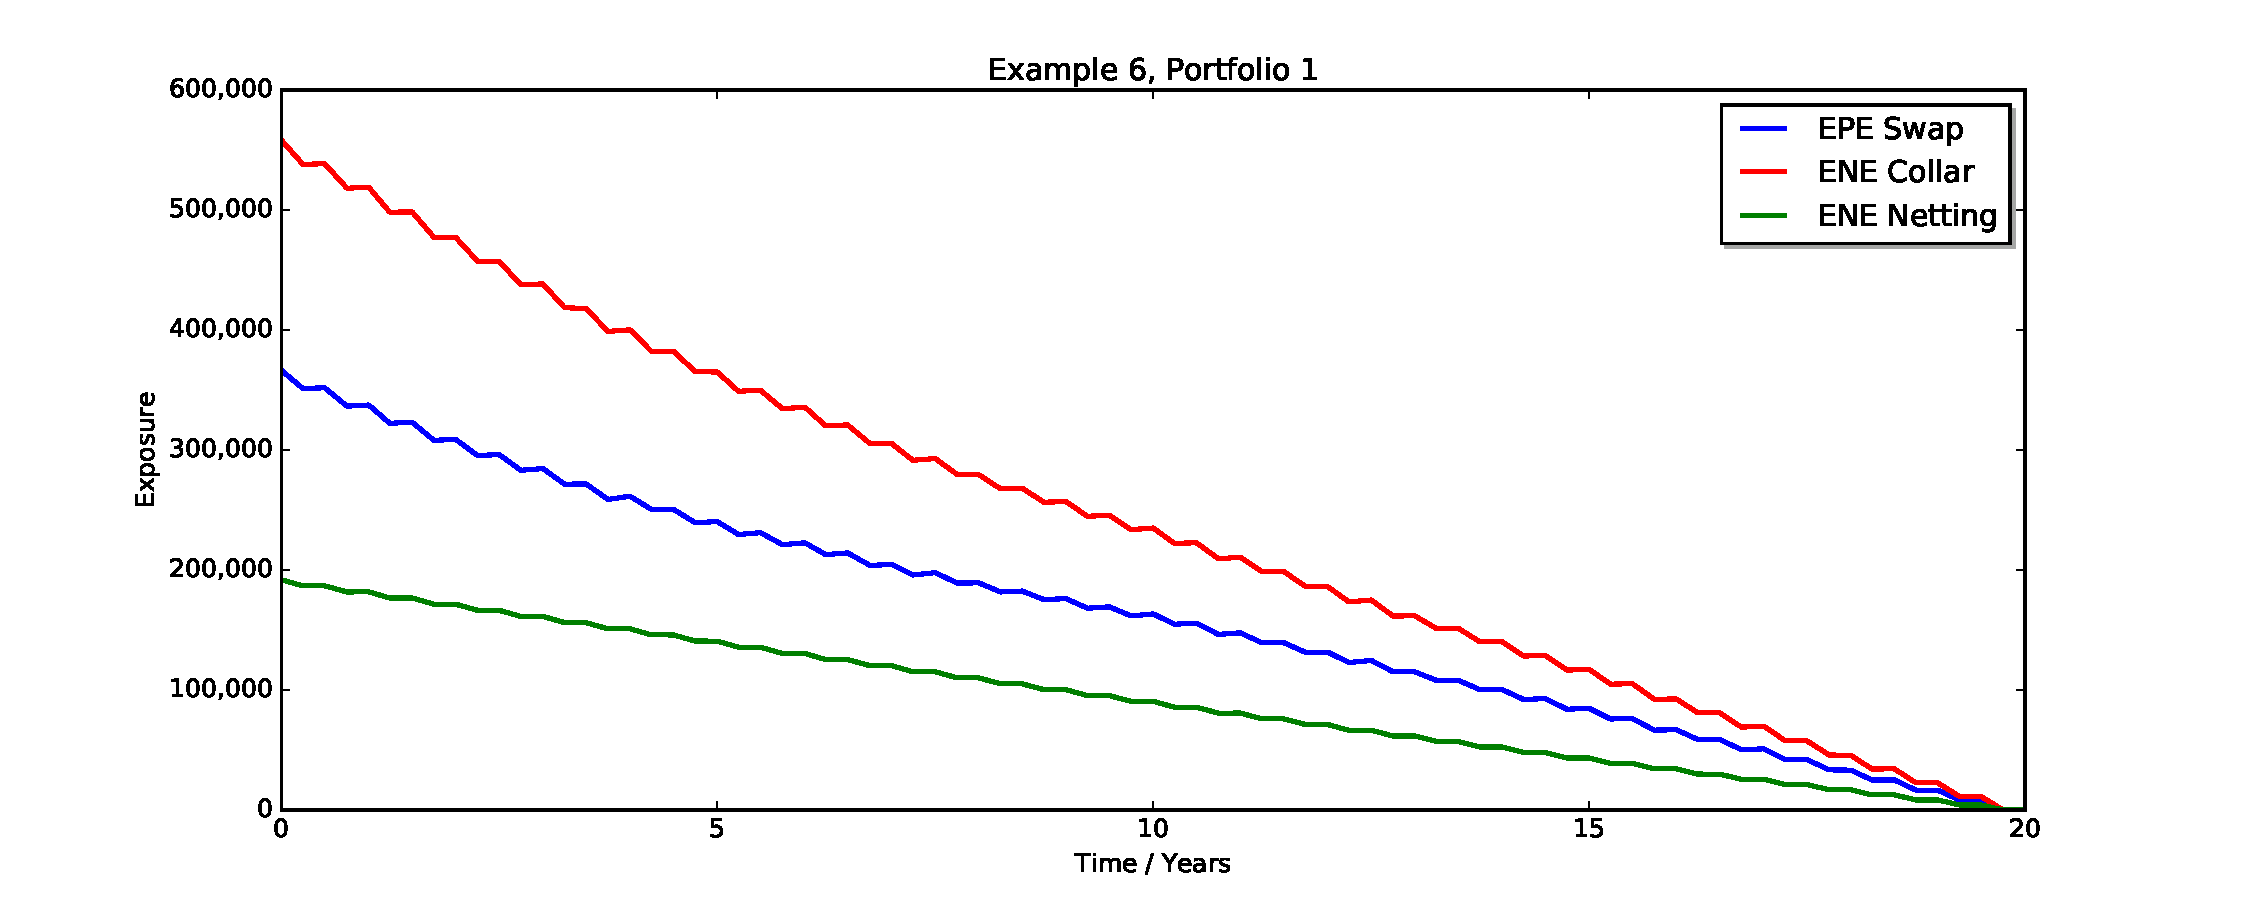
\includegraphics[scale=0.45]{examples/mpl_capfloor_1.pdf}
\end{center}
\caption{Swap+Collar, portfolio 1. The Collar has identical cap and floor rates at 4\% so that it corresponds to a
  fixed leg which reduces the exposure of the Swap, which receives 3\% fixed. Simulation with 1000 paths and quarterly
  time steps.}
\label{fig_capfloor_1}
\end{figure}

The second example in this folder shown in figure \ref{fig_capfloor_2} ('portfolio 2') consists of a short Cap, long
Floor and a long Collar that exactly offsets the netted Cap and Floor.

\begin{figure}[h!]
\begin{center}
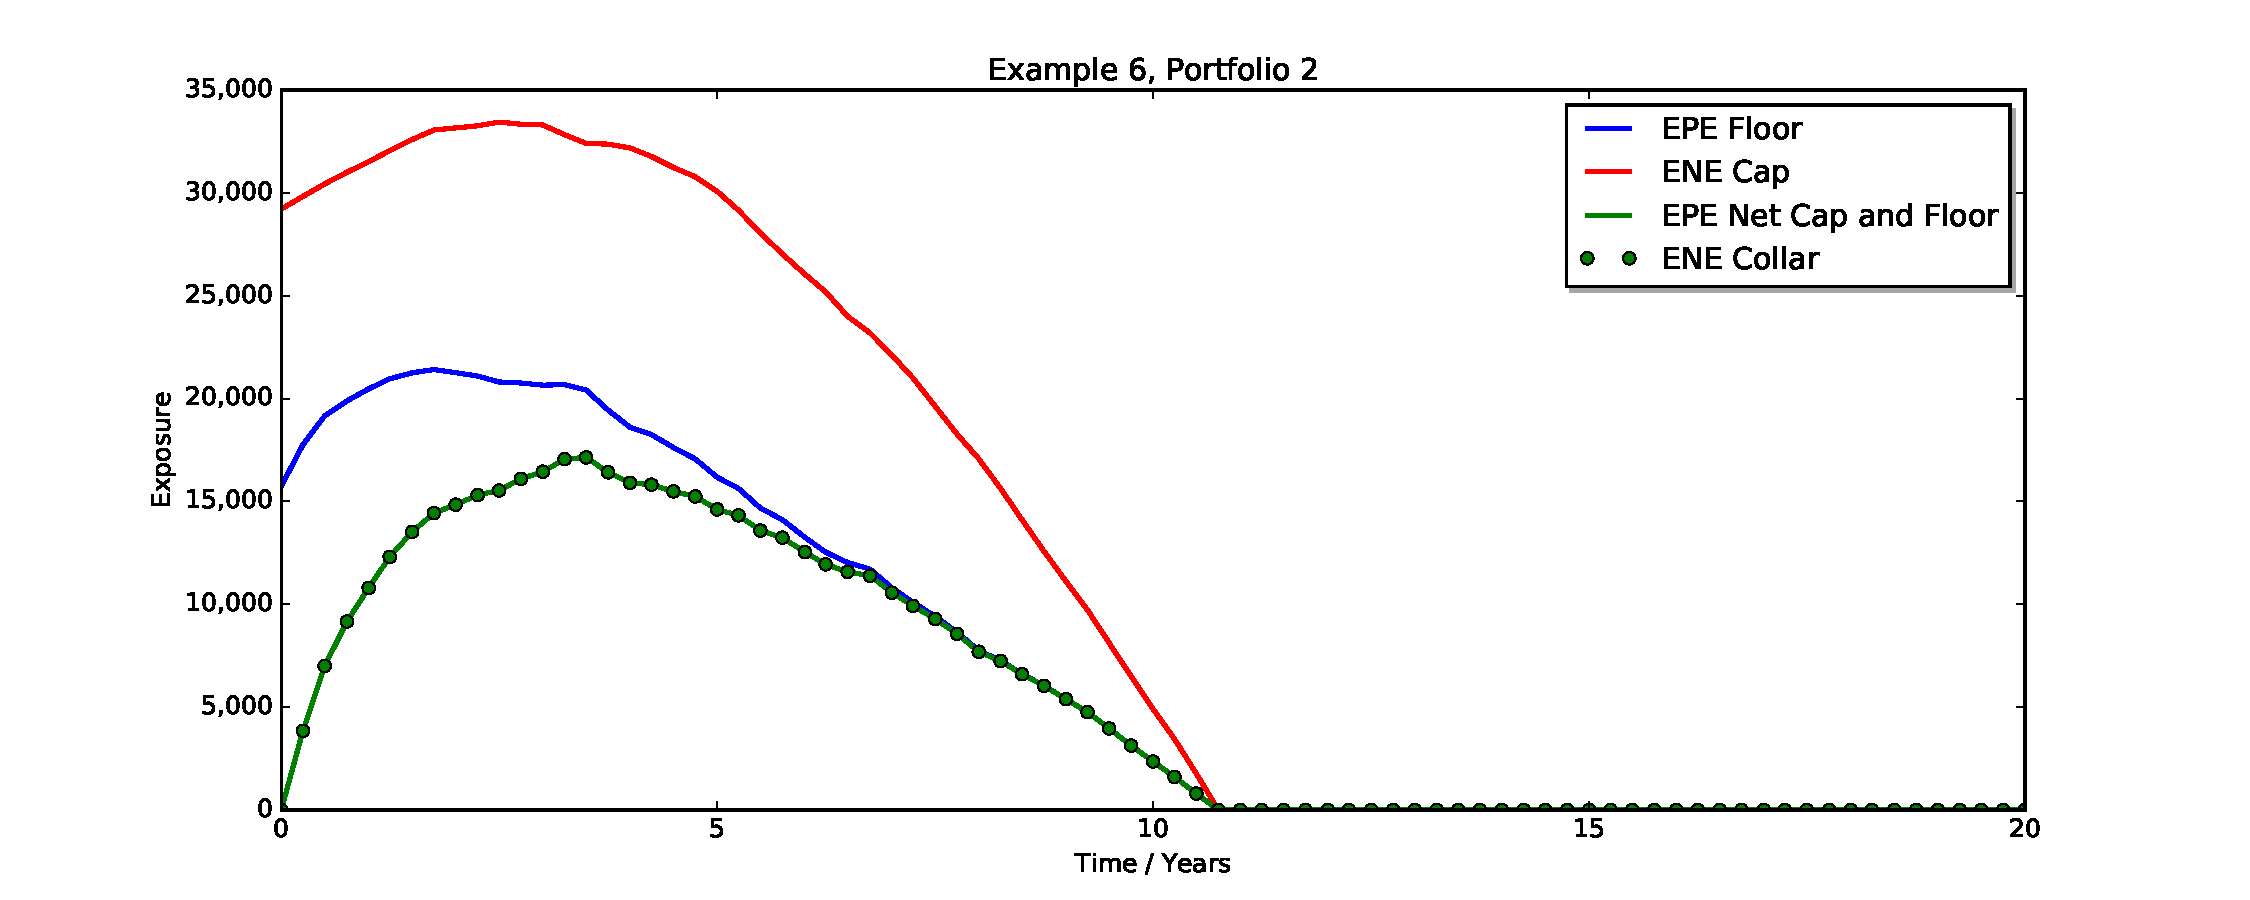
\includegraphics[scale=0.45]{examples/mpl_capfloor_2.pdf}
\end{center}
\caption{Short Cap and long Floor vs long Collar, portfolio 2. Simulation with 1000 paths and quarterly time steps.}
\label{fig_capfloor_2}
\end{figure}

Further three test portfolios are provided as part of this example. Run the example and inspect the respective output
directories {\tt Examples/Exposure/Output/capfloor/portfolio\_\#}. 

\subsubsection{FX Forward and FX Option}\label{example:exposure_fx}

Example {\tt python run\_fx.py} generates the exposure evolution for a EUR / USD FX Forward transaction
with value date in 10Y. This is a particularly simple show case because of the single cash flow in 10Y. On the other
hand it checks the cross currency model implementation by means of comparison to analytic limits - EPE and ENE at the
trade's value date must match corresponding Vanilla FX Option prices, as shown in figure \ref{fig_5}.
\begin{figure}[h]
\begin{center}
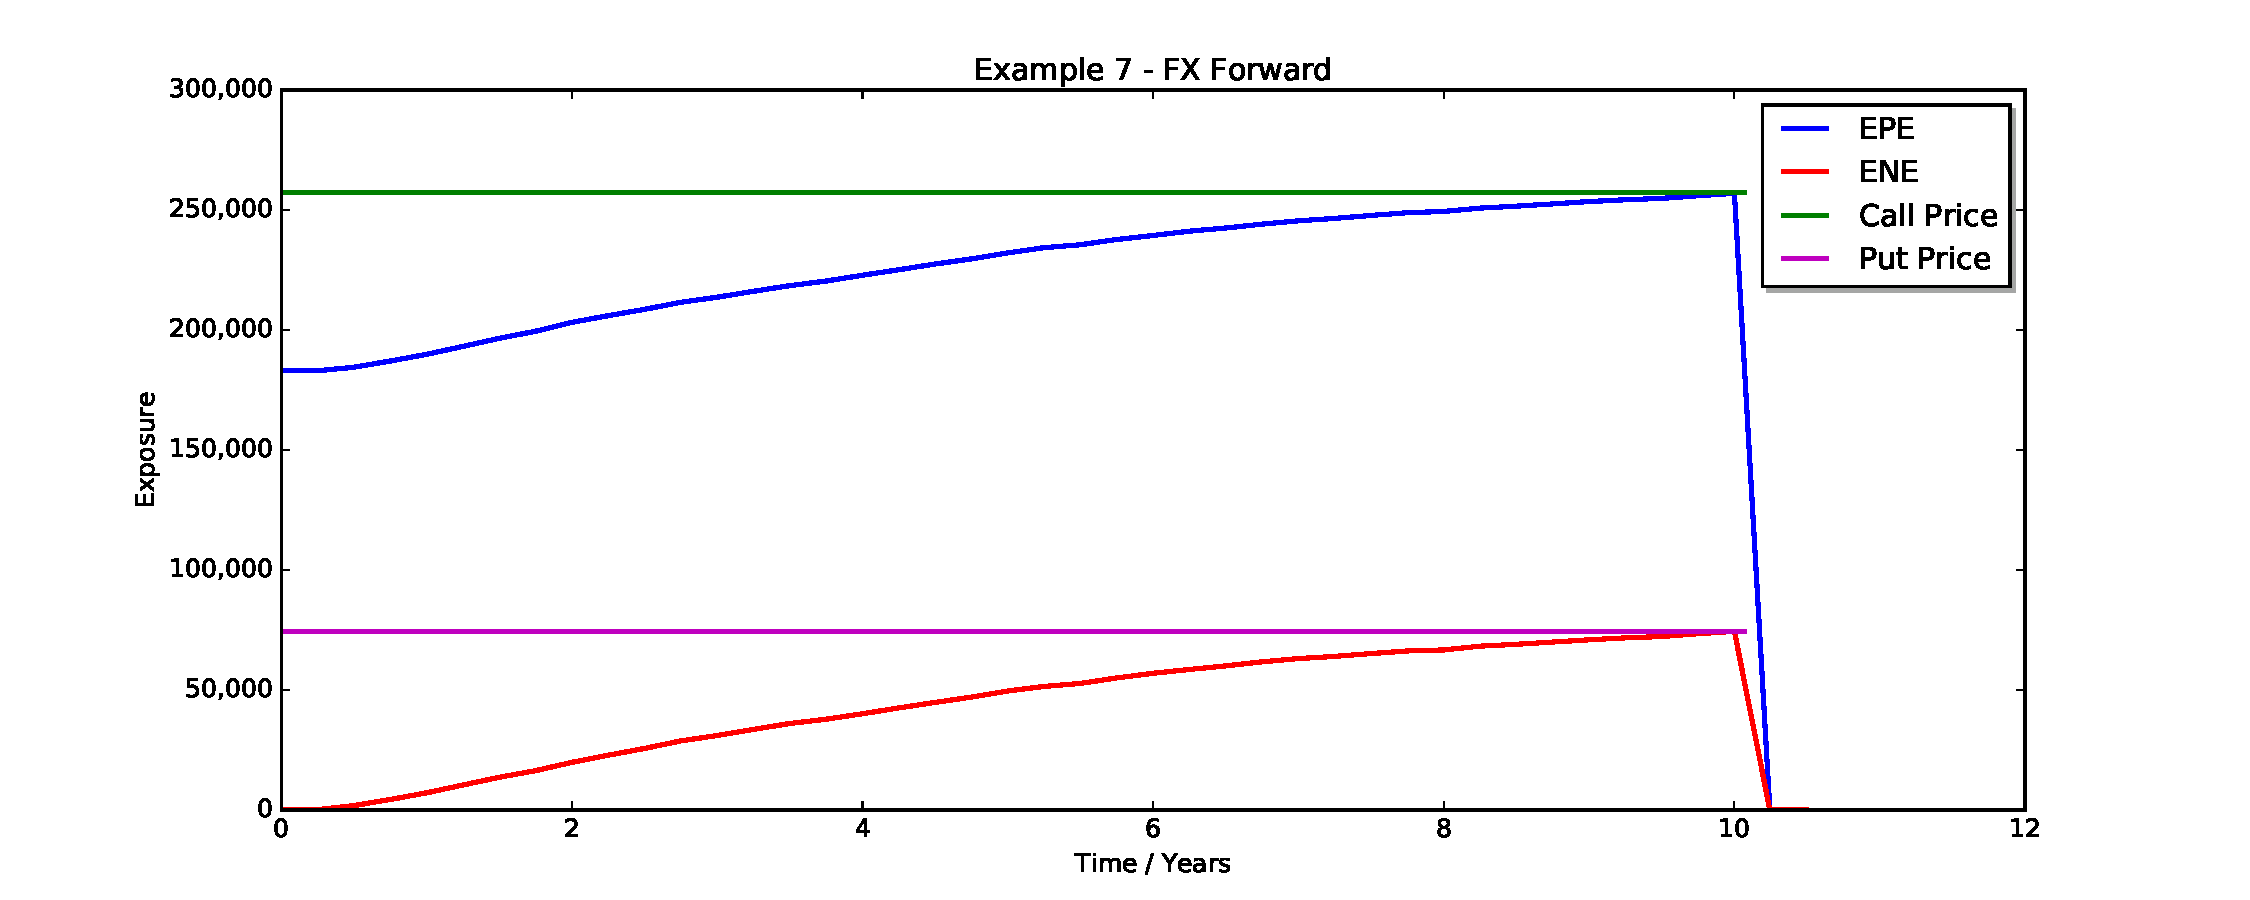
\includegraphics[scale=0.45]{examples/mpl_fxforward.pdf}
\end{center}
\caption{EUR/USD FX Forward expected exposure in a realistic market environment as of 26/02/2016 from both parties'
  perspectives. Value date is obviously in 10Y. The flat lines are FX Option prices which coincide with EPE and ENE,
  respectively, on the value date. Simulation with 5000 paths and quarterly time steps.}
\label{fig_5}
\end{figure}

The same batch illustrates the exposure evolution for an FX Option, see figure \ref{fig_7}.
\begin{figure}[h!]
\begin{center}
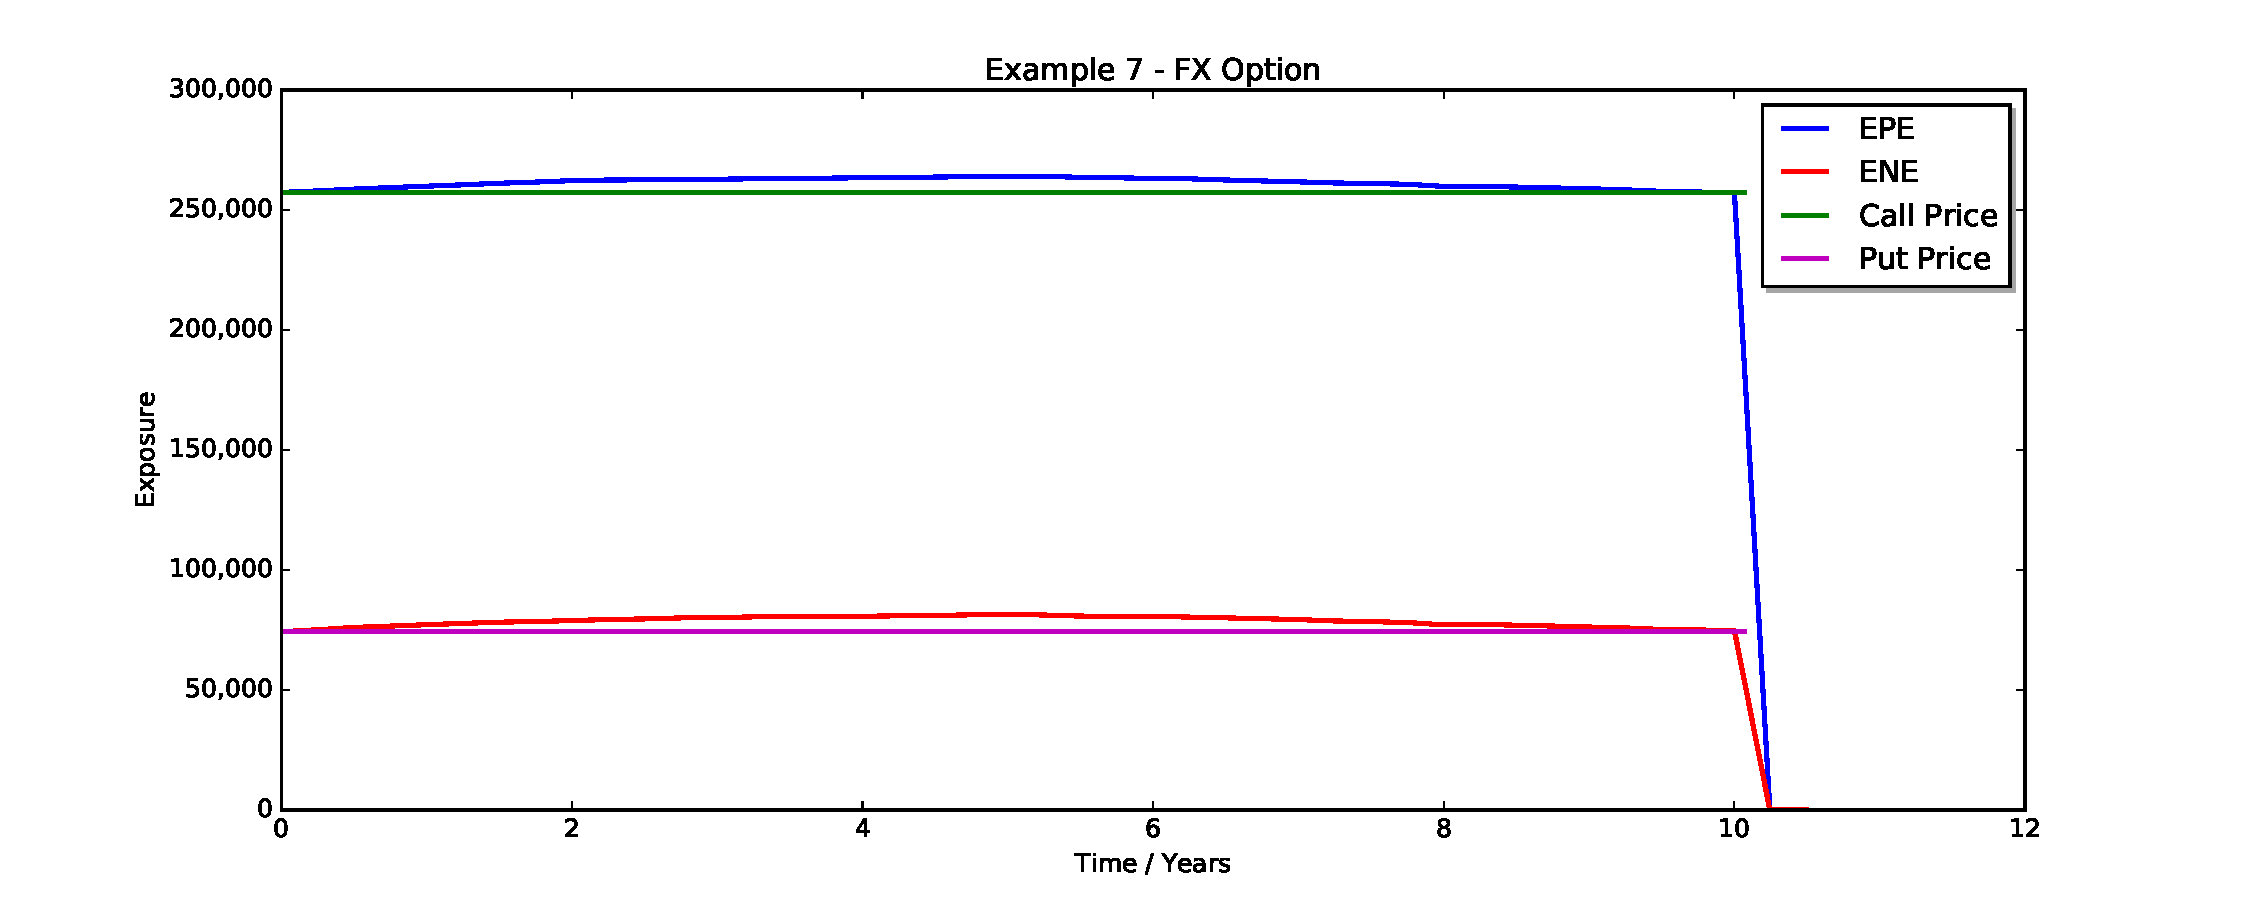
\includegraphics[scale=0.45]{examples/mpl_fxoption.pdf}
\end{center}
\caption{EUR/USD FX Call and Put Option exposure evolution, same underlying and market data as above,
  compared to the call and put option price as of today (flat line). Simulation with 5000 paths and
  quarterly time steps.}
\label{fig_7}
\end{figure}
Recall that the FX Option value $NPV(t)$ as of time $0 \leq t \leq T$ satisfies
\begin{align*}
\frac{NPV(t)}{N(t)} &= \mbox{Nominal}\times\E_t\left[\frac{(X(T) - K)^+}{N(T)}\right]\\
NPV(0) &= \E\left[\frac{NPV(t)}{N(t)}\right] = \E\left[\frac{NPV^+(t)}{N(t)} \right]= \EPE(t) 
\end{align*}
where $N(t)$ denotes the numeraire asset.
One would therefore expect a flat exposure evolution up to option expiry. The deviation from this in ORE's simulation is
due to the pricing approach chosen here under scenarios. A Black FX option pricer is used with deterministic Black
volatility derived from today's volatility structure (pushed or rolled forward, see section \ref{sec:sim_market}). The
deviation can be removed by extending the volatility modelling, e.g. implying model consistent Black volatilities in
each simulation step on each path.  

\subsubsection{Non-Resetting and Resetting Cross Currency Swaps}\label{example:exposure_ccs}

Batch {\tt run\_ccs.py} demonstrates a vanilla non-resetting cross currency Swap exposure.
It shows the typical blend of an Interest Rate Swap's saw tooth exposure evolution with an FX Forward's exposure
which increases monotonically to final maturity, see
figure \ref{fig_6}.
\begin{figure}[h!]
\begin{center}
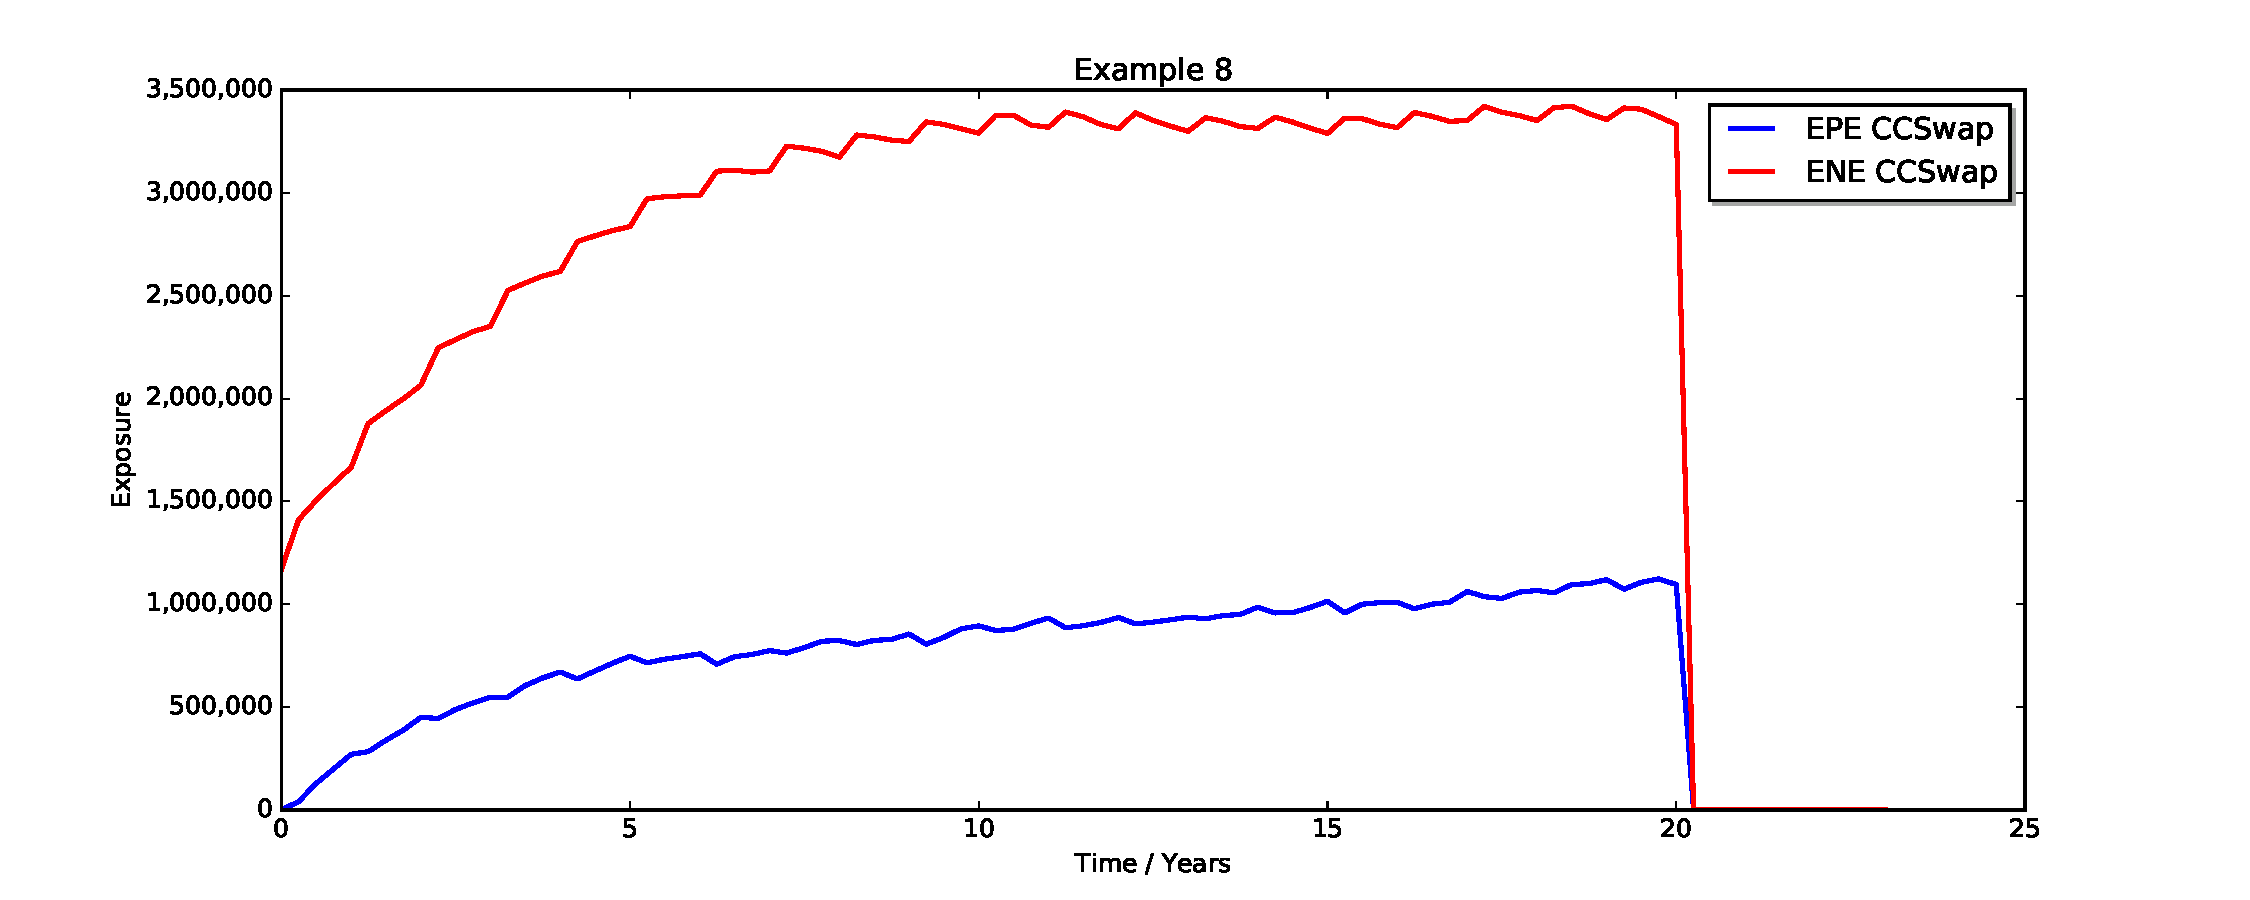
\includegraphics[scale=0.45]{examples/mpl_ccswap.pdf}
\end{center}
\caption{Cross Currency Swap exposure evolution without mark-to-market notional reset. Simulation with 1000 paths and
  quarterly time steps.}
\label{fig_6}
\end{figure}

This run also demonstrates the ``serialization'' of the calibrated simulation model, see {\tt Output/swaption/calibration.xml}
and {\tt Output/swaption/calibration.csv}, as well as the brief documentation of the {\tt calibration} analytic
in section \ref{sec:analytics}.

Finally, the effect of the FX resetting feature, common in Cross Currency Swaps nowadays, is also demonstrated here using a
separate instrument (see {\tt portfolio\_ccs.xml}).
The example shows the exposure evolution of a EUR/USD cross currency basis Swap with FX reset at each interest period
start, see figure \ref{fig_6b}. As expected, the notional reset causes an exposure collapse at each period start when
the EUR leg's notional is reset to match the USD notional.
\begin{figure}[h!]
\begin{center}
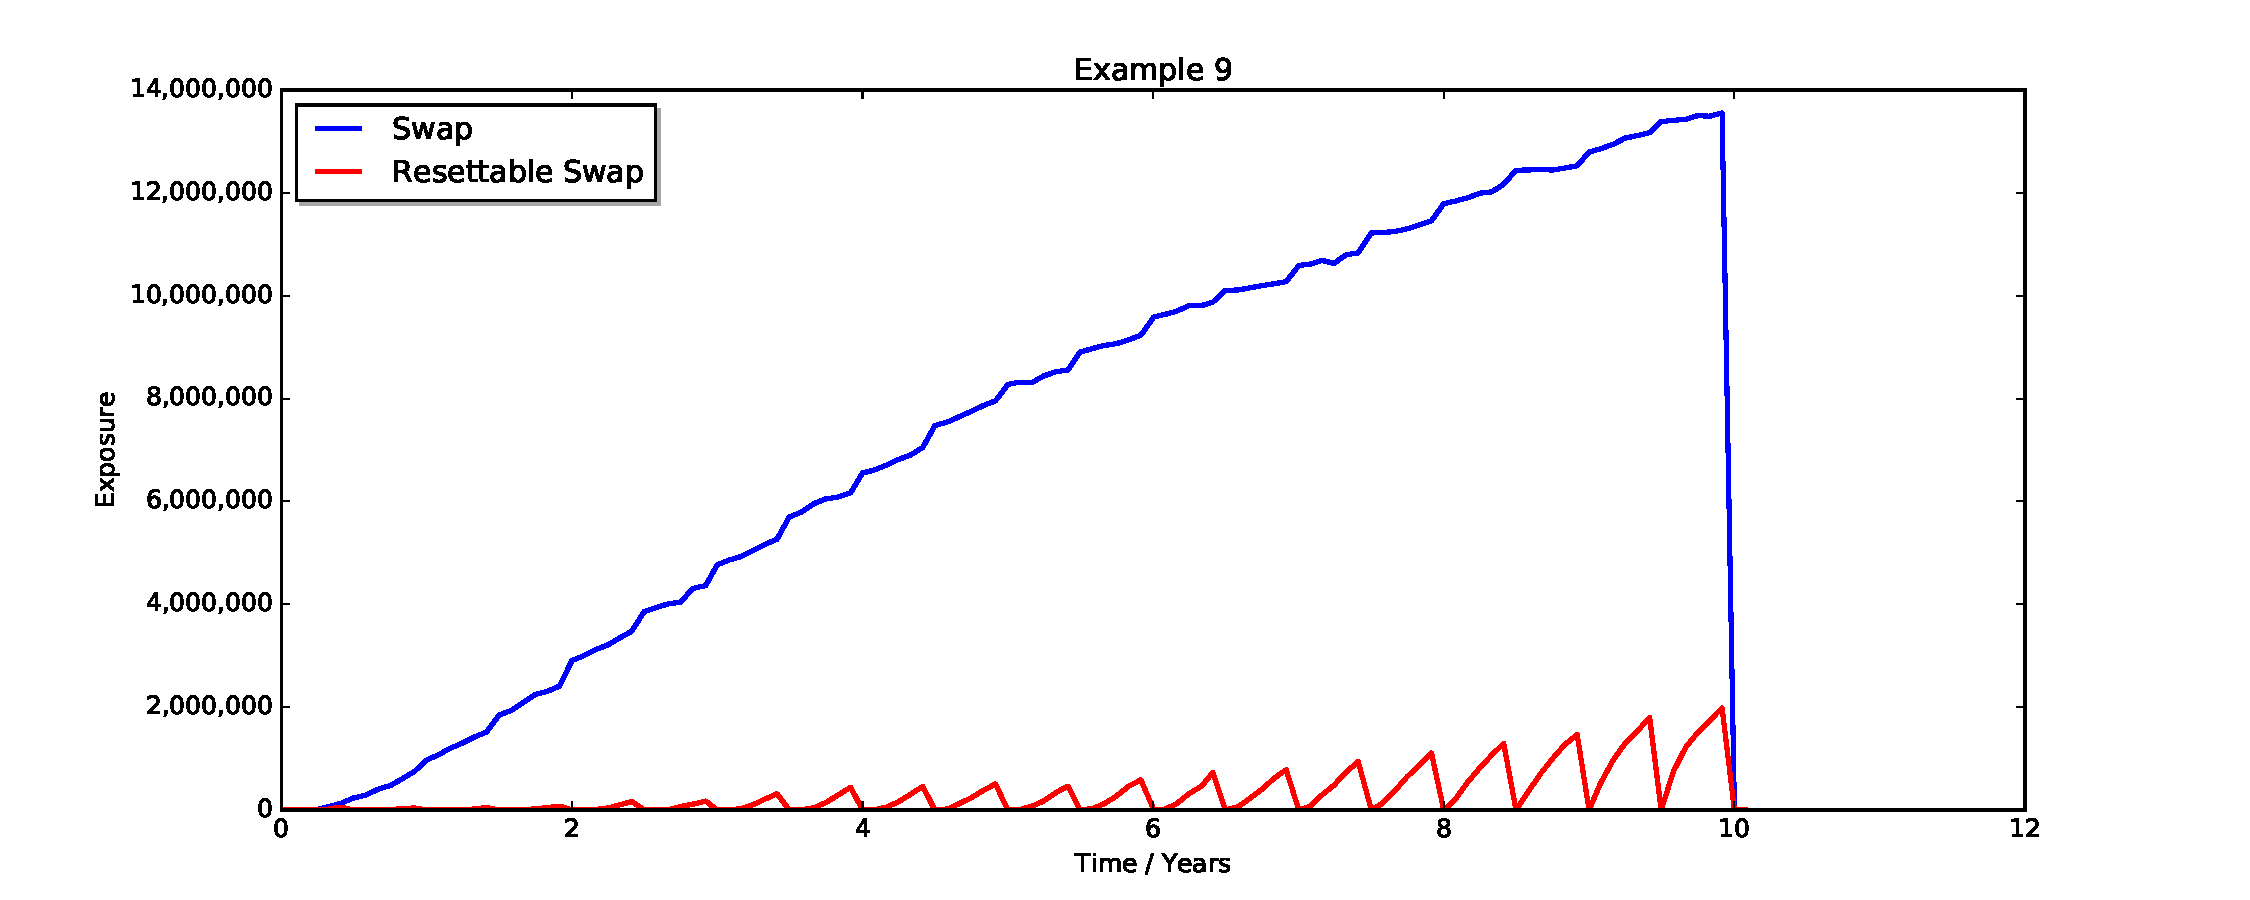
\includegraphics[scale=0.45]{examples/mpl_xccy_reset.pdf}
\end{center}
\caption{Cross Currency Basis Swap exposure evolution with and without mark-to-market notional reset. Simulation with
  1000 paths and quarterly time steps.}
\label{fig_6b}
\end{figure}

\subsubsection{Equity Derivatives}\label{example:exposure_equity}

This example in {\tt python run\_equity.py} demonstrates the computation of NPV, sensitivities, exposures and XVA for a portfolio 
of OTC equity derivatives. The portfolio used in this example consists of:

\begin{itemize}
	\item an equity call option denominated in EUR (``Luft'')
	\item an equity put option denominated in EUR (``Luft'')
	\item an equity forward denominated in EUR (``Luft'')
	\item an equity call option denominated in USD (``SP5'')
	\item an equity put option denominated in USD (``SP5'')
	\item an equity forward denominated in USD (``SP5'')
	\item an equity Swap in USD with return type  ``price'' (``SP5'')
	\item an equity Swap in USD with return type ``total'' (``SP5'')
\end{itemize}

The step-by-step procedure for running ORE is identical for equities as for other asset classes; the same market and 
portfolio data files are used to store the equity market data and trade details, respectively. For the exposure 
simulation, the calibration parameters for the equity risk factors can be set in the usual {\tt simulation.xml} file.

Looking at the MtM results in the output file {\tt npv.csv} we observe that put-call parity ($V_{Fwd} = V_{Call} - 
V_{Put}$) is observed as expected. Looking at Figure \ref{fig_eq_call} we observe that the Expected Exposure profile of 
the equity call option trade is relatively smooth over time, while for the equity forward trade the Expected Exposure 
tends to increase as we approach maturity. This behaviour is similar to what we observe in section \ref{example:exposure_fx}.

\begin{figure}[h!]
  \begin{center}
    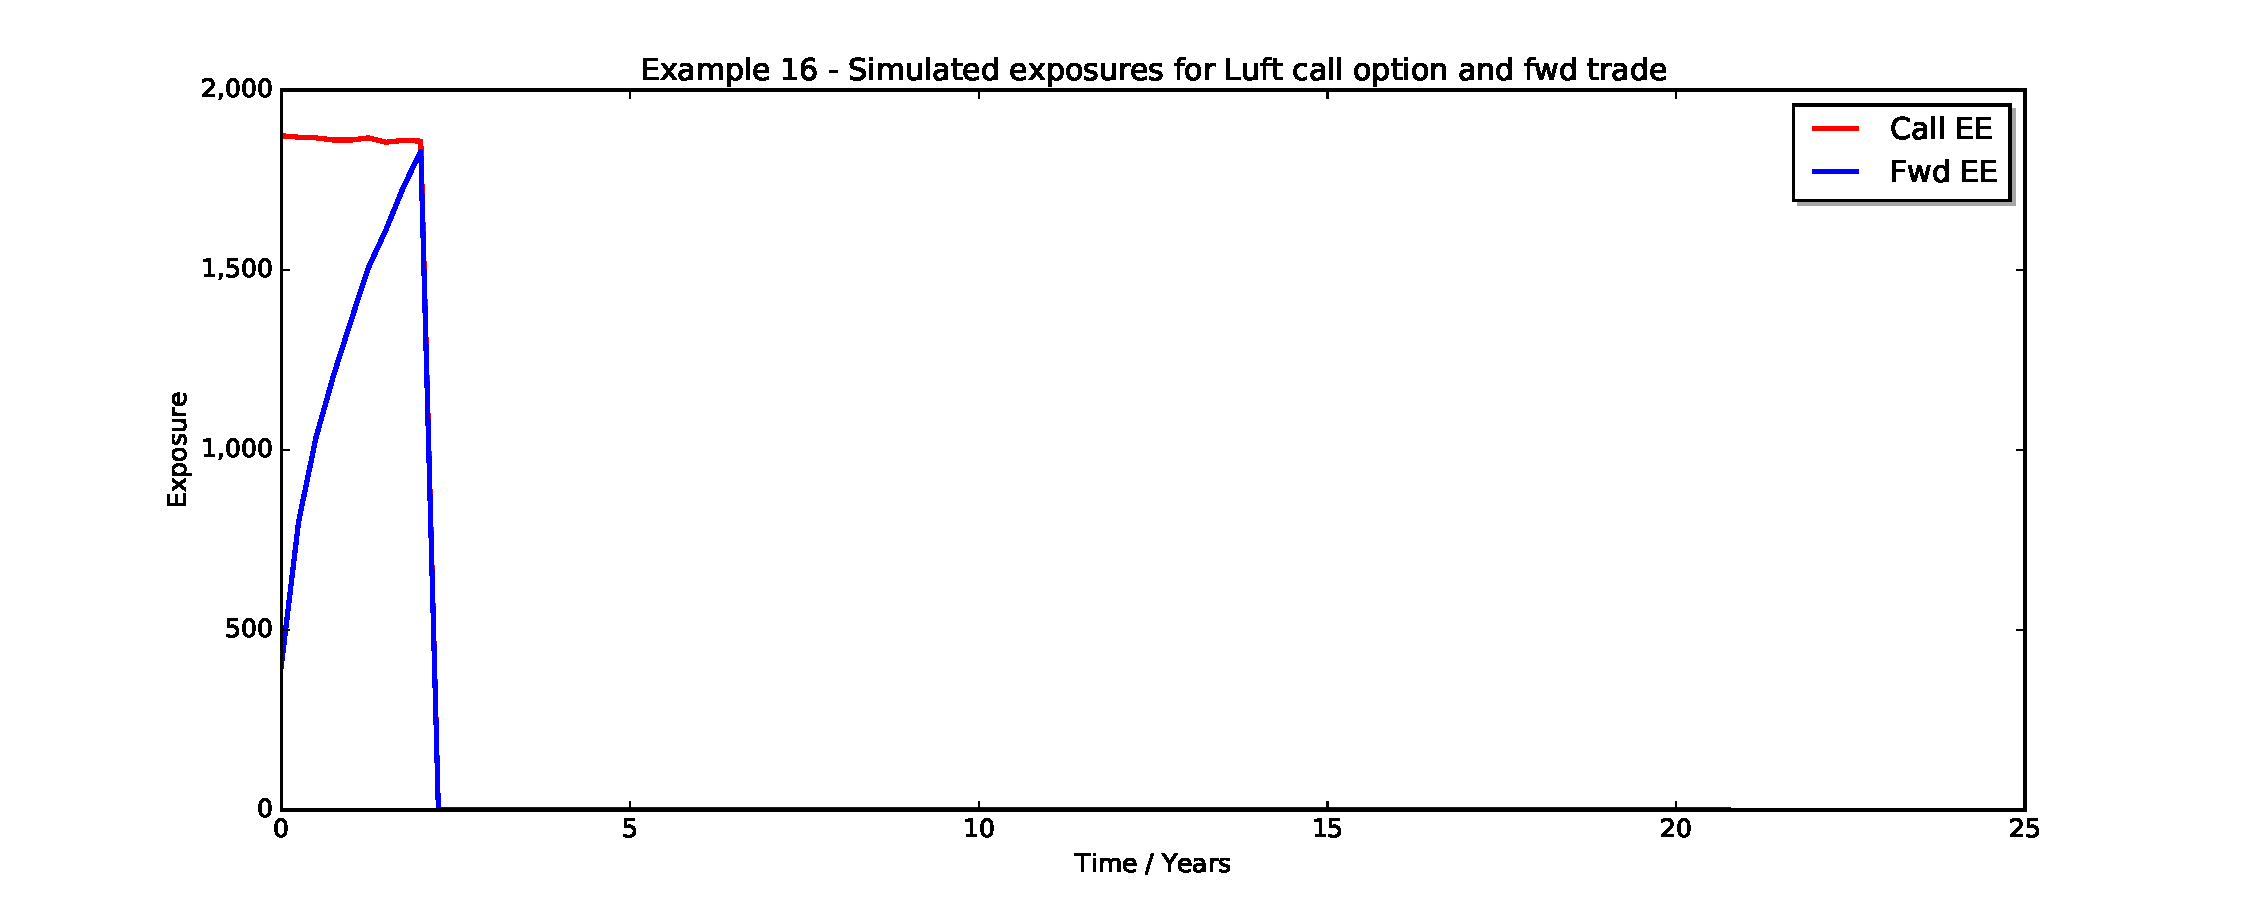
\includegraphics[scale=0.45]{examples/mpl_eq_call.pdf}
  \end{center}
  \caption{Equity (``Luft'') call option and OTC forward exposure evolution, maturity in approximately 2.5 years. 
    Simulation with 
    10000 paths and quarterly time steps.}
  \label{fig_eq_call}
\end{figure}

\subsubsection{Commodity Derivatives}\label{example:exposure_commodity}

Calling

\medskip
\centerline{\tt python run\_commodity.py}

\medskip
demonstrates pricing and exposure simulation for a portfolio including a
\begin{itemize}
\item Commodity Forward
\item Commodity Swap
\item European Commodity Option
\item Commodity Average Price Option
\item Commodity Swaption
\end{itemize}
with the usual results, exposure reports and graphs. 

\subsubsection{Inflation CPI and YOY Swap - TODO}\label{example:exposure_inflation}

The example called with {\tt python run\_inflation.py} runs two exposure simulation batches for CPI and YOY Inflation Swaps
\begin{itemize}
\item using the Dodgson-Kainth (DK) inflation model
\item using the Jarrow-Yildirim (JY) inflation model
\end{itemize}

We use the same portfolio in both batches that comprises four trades
\begin{itemize}
\item EU and UK CPI Swaps
\item EU and UK YOY Swaps
\end{itemize}

Figures \ref{fig_inflation_dk} and \ref{fig_inflation_jy} show the exposure (EPE) graphs for all trades.

\begin{figure}[h!]
  \begin{center}
    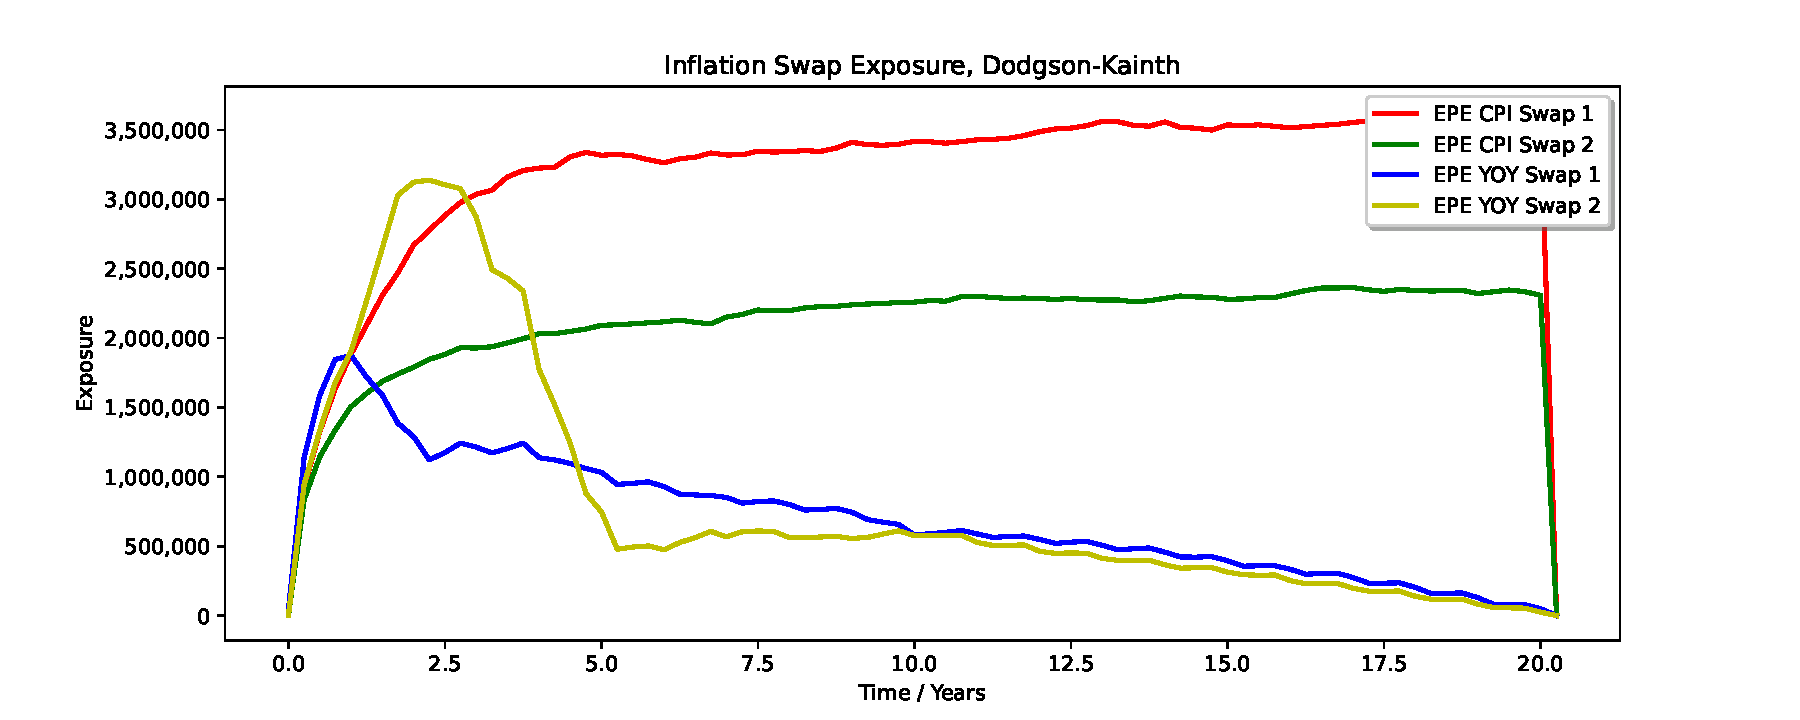
\includegraphics[scale=0.45]{examples/mpl_exposure_inflation_dk.pdf}
  \end{center}
  \caption{CPI and YOY exposure evolution using the Dodgson-Kainth model.}
  \label{fig_inflation_dk}
\end{figure}

\begin{figure}[h!]
  \begin{center}
    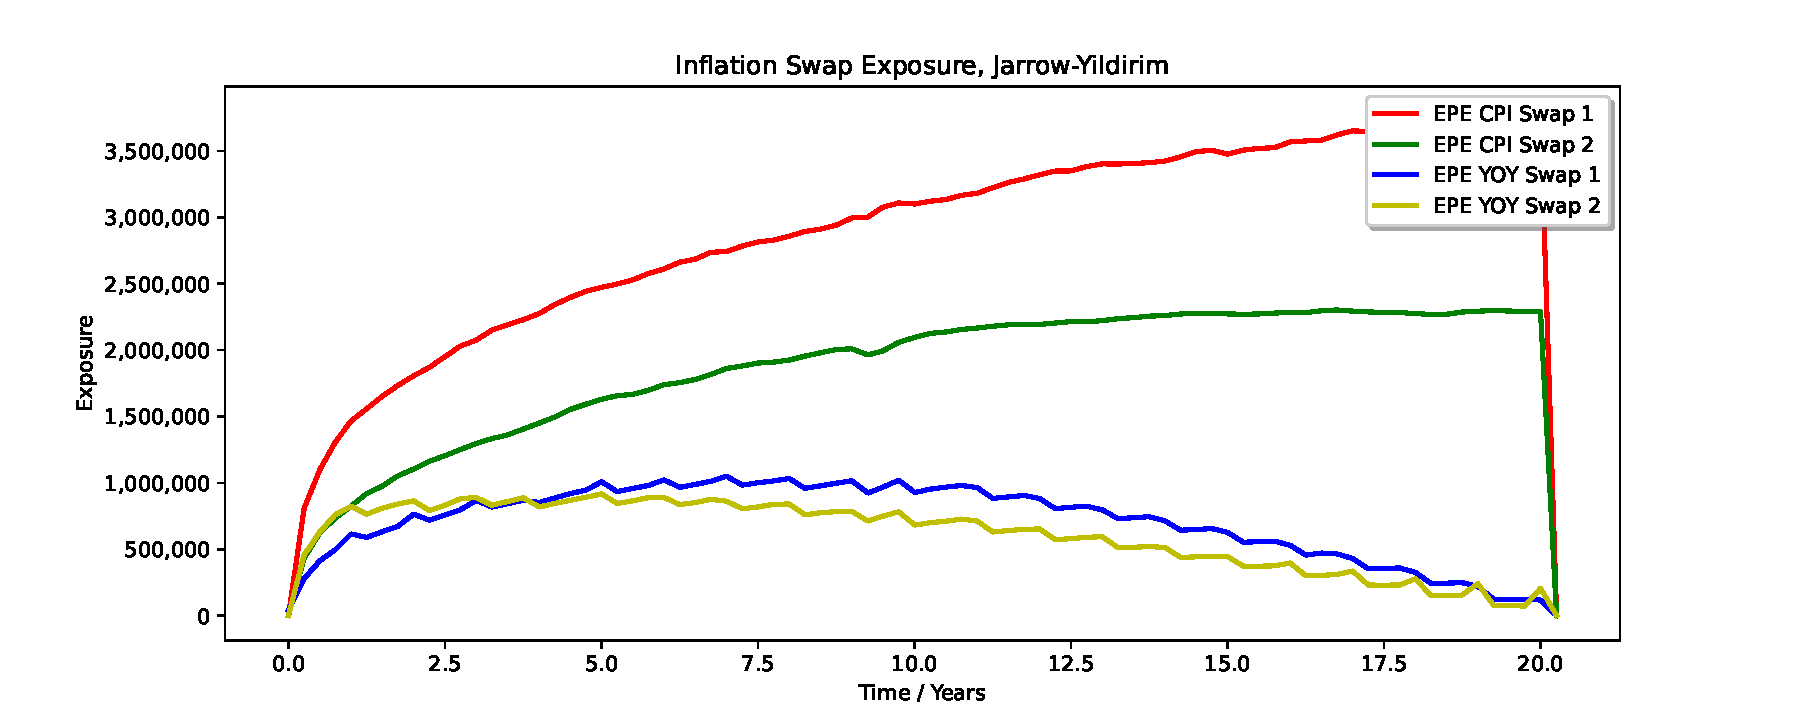
\includegraphics[scale=0.45]{examples/mpl_exposure_inflation_jy.pdf}
  \end{center}
  \caption{CPI and YOY exposure evolution using the Jarrow-Yildirim model.}
  \label{fig_inflation_jy}
\end{figure}

TODO: Discuss differences, check model calibrations

\subsubsection{Credit Default Swap}\label{example:exposure_credit}

Calling

\medskip
\centerline{\tt python run\_credit.py } 
\medskip

runs the credit variant of the Swap exposure in \ref{example:exposure_swapflat}.
Running ORE here yields the exposure evolution shown in figure \ref{fig_33}. 
\begin{figure}[h!]
\begin{center}
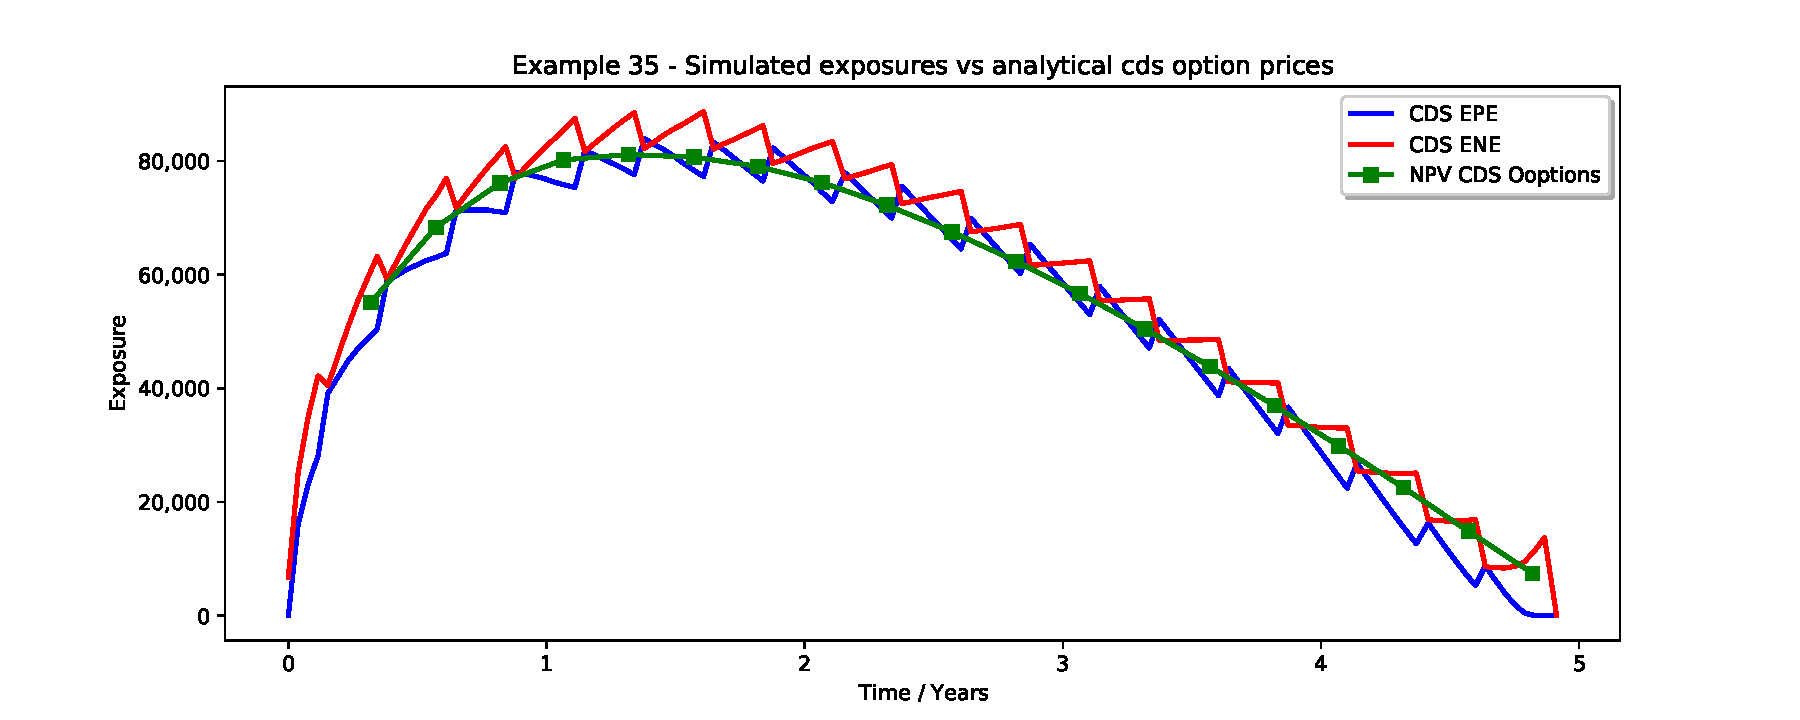
\includegraphics[scale=0.45]{examples/mpl_cds_33_2w_10k.pdf}
\end{center}
\caption{Credit Default Swap expected exposure in a flat market environment from both parties' perspectives. The symbols are CDS Option prices. The simulation was run with bi-weekly time steps and 10,000 Monte Carlo samples to demonstrate the convergence of EPE and ENE profiles. A similar
outcome can be obtained more quickly with 5,000 samples on a monthly time grid which is the default setting  here. }
\label{fig_33}
\end{figure}
Both CDS simulation and CDS Option pricing are run with calls to the ORE executable, essentially 

\medskip
\centerline{\tt ore[.exe] ore\_credit.xml} 

\centerline{\tt ore[.exe] ore\_creditoptions.xml} 
\medskip

which are wrapped into the script {\tt Examples/Eposure/run\_credit.py} provided with the ORE release.

This example demonstrates credit simulation using the LGM model and the calculation of Wrong Way Risk due to credit
correlation between the underlying entity of the CDS and the counterparty of the CDS trade via dynamic credit.
Positive correlation between the two names weakens the protection of the CDS whilst
negative correlation strengthens the protection.

The following table lists the XVA result from the example at different levels of correlation.

\begin{table}[hbt]
\scriptsize
\begin{center}
\begin{tabular}{|r|l|r|r|r|r|}
\hline
Correlation & NettingSetId & CVA & DVA & FBA & FCA \\
\hline
-100\%  &  CPTY\_B  &  -2,638  &  2,906  &  486  &  -1,057 \\
 -90\%  &  CPTY\_B  &  -2,204  &  2,906  &  488  &  -1,053 \\
 -50\%  &  CPTY\_B  &    -485  &  2,906  &  493  &  -1,040 \\
 -40\%  &  CPTY\_B  &     -60  &  2,906  &  495  &  -1,037 \\
 -30\%  &  CPTY\_B  &     363  &  2,906  &  496  &  -1,033 \\
 -20\%  &  CPTY\_B  &     784  &  2,906  &  498  &  -1,030 \\
 -10\%  &  CPTY\_B  &   1,204  &  2,906  &  500  &  -1,027 \\
   0\%  &  CPTY\_B  &   1,621  &  2,906  &  501  &  -1,023 \\
  10\%  &  CPTY\_B  &   2,036  &  2,906  &  503  &  -1,020 \\
  20\%  &  CPTY\_B  &   2,450  &  2,906  &  504  &  -1,017 \\
  30\%  &  CPTY\_B  &   2,861  &  2,906  &  506  &  -1,013 \\
  40\%  &  CPTY\_B  &   3,271  &  2,906  &  507  &  -1,010 \\
  50\%  &  CPTY\_B  &   3,679  &  2,906  &  509  &  -1,017 \\
  90\%  &  CPTY\_B  &   5,290  &  2,906  &  515  &    -994 \\
 100\%  &  CPTY\_B  &   5,689  &  2,906  &  517  &    -991 \\
\hline
\end{tabular}
\caption{CDS XVA results with LGM model}
\end{center}
\end{table}

\subsubsection{Capped/Floored (Digital) CMS Spread}\label{example:exposure_cmsspread}

Calling

\medskip
\centerline{\tt python run\_cmsspread.py } 
\medskip

runs pricing and exosure simulation for 
\begin{itemize}
\item Capped/Floored CMS Spreads
\item CMS Spreads with Digital Caps/Floors
\end{itemize}

Results are found in folder {\tt Examples/Exposure/Output/cmsspread/*} and exposure graphs in {\tt Examples/Exposure/Output/mpl\_cmsspread.pdf}.

\subsubsection{Capped (Digital) CMS Spread with Formula-based Payoff}\label{example:exposure_fbc}

Calling

\medskip
\centerline{\tt python run\_fbc.py } 
\medskip

runs pricing, exosure simulation and XVA for Swaps with CMS Spread and
Digital CMS Spread legs using both formula-based payoff and ``classic'' ORE XML.
The example portfolio also includes a Bond with formula-based payoff.
Results are found in folder {\tt Examples/Exposure/Output/fbc/*}

The formula-based leg can be seen as a predecessor of the more versatile
scripted trade framework. However, the formula leg may be used to
apply a multi-factor Log-normal Swap Rate model instead of the Gaussian
interest rate models currently applied in the scripted trade framework.

\subsubsection{Long-term simulation}\label{example:exposure_longterm}

Calling

\medskip
\centerline{\tt python run\_longterm.py } 
\medskip

demonstrates an effect that, at first glance, seems to cause a serious issue with long term simulations.
Fortunately this can be avoided quite easily in the Linear Gauss Markov model setting
that is used here. \\

In the example we consider a Swap with maturity in 50 years in a flat yield curve environment. If we simulate this
naively as in all previous cases, we obtain a particularly noisy EPE profile that does not nearly reconcile with the
known exposure (analytical Swaption prices). This is shown in figure \ref{fig_15} (`no horizon shift'). The origin of
this issue is the width of the risk-neutral NPV distribution at long time horizons which can turn out to be quite small
so that the Monte Carlo simulation with finite number of samples does not reach far enough into the positive or negative
NPV range to adequately sample the distribution, and estimate both EPE and ENE in a single run.  Increasing the number
of samples may not solve the problem, and may not even be feasible in a realistic setting. \\

The way out is applying a `shift transformation' to the Linear Gauss Markov model, see {\tt
  Exposure/Input/simulation\_longterm\_2.xml} in lines 92-95:
\begin{listing}[H]
%\hrule\medskip
\begin{minted}[fontsize=\footnotesize]{xml}
        <ParameterTransformation>
          <ShiftHorizon>30.0</ShiftHorizon>
          <Scaling>1.0</Scaling>
        </ParameterTransformation>
\end{minted}
%\hrule
%\caption{LGM Shift transformation}
%\label{lst:shift_transformation}
\end{listing}

The effect of the 'ShiftHorizon' parameter $T$ is to apply a shift to the Linear Gauss Markov model's $H(t)$ parameter
(see \cite{methods}) {\em after} the model has been calibrated, i.e. to replace:
$$ 
H(t) \rightarrow H(t) - H(T) 
$$ 
It can be shown that this leaves all expectations computed in the model (such as EPE and ENE) invariant. As explained in
\cite{Lichters}, subtracting an $H$ shift effectively means performing a change of measure from the `native' LGM measure
to a T-Forward measure with horizon $T$, here 30 years. Both negative and positive shifts are permissible, but only
negative shifts are connected with a T-Forward measure and improve numerical stability. \\

In our experience it is helpful to place the horizon in the middle of the portfolio duration to significantly improve
the quality of long term expectations. The effect of this change (only) is shown in the same figure \ref{fig_15}
(`shifted horizon').
\begin{figure}[h!]
\begin{center}
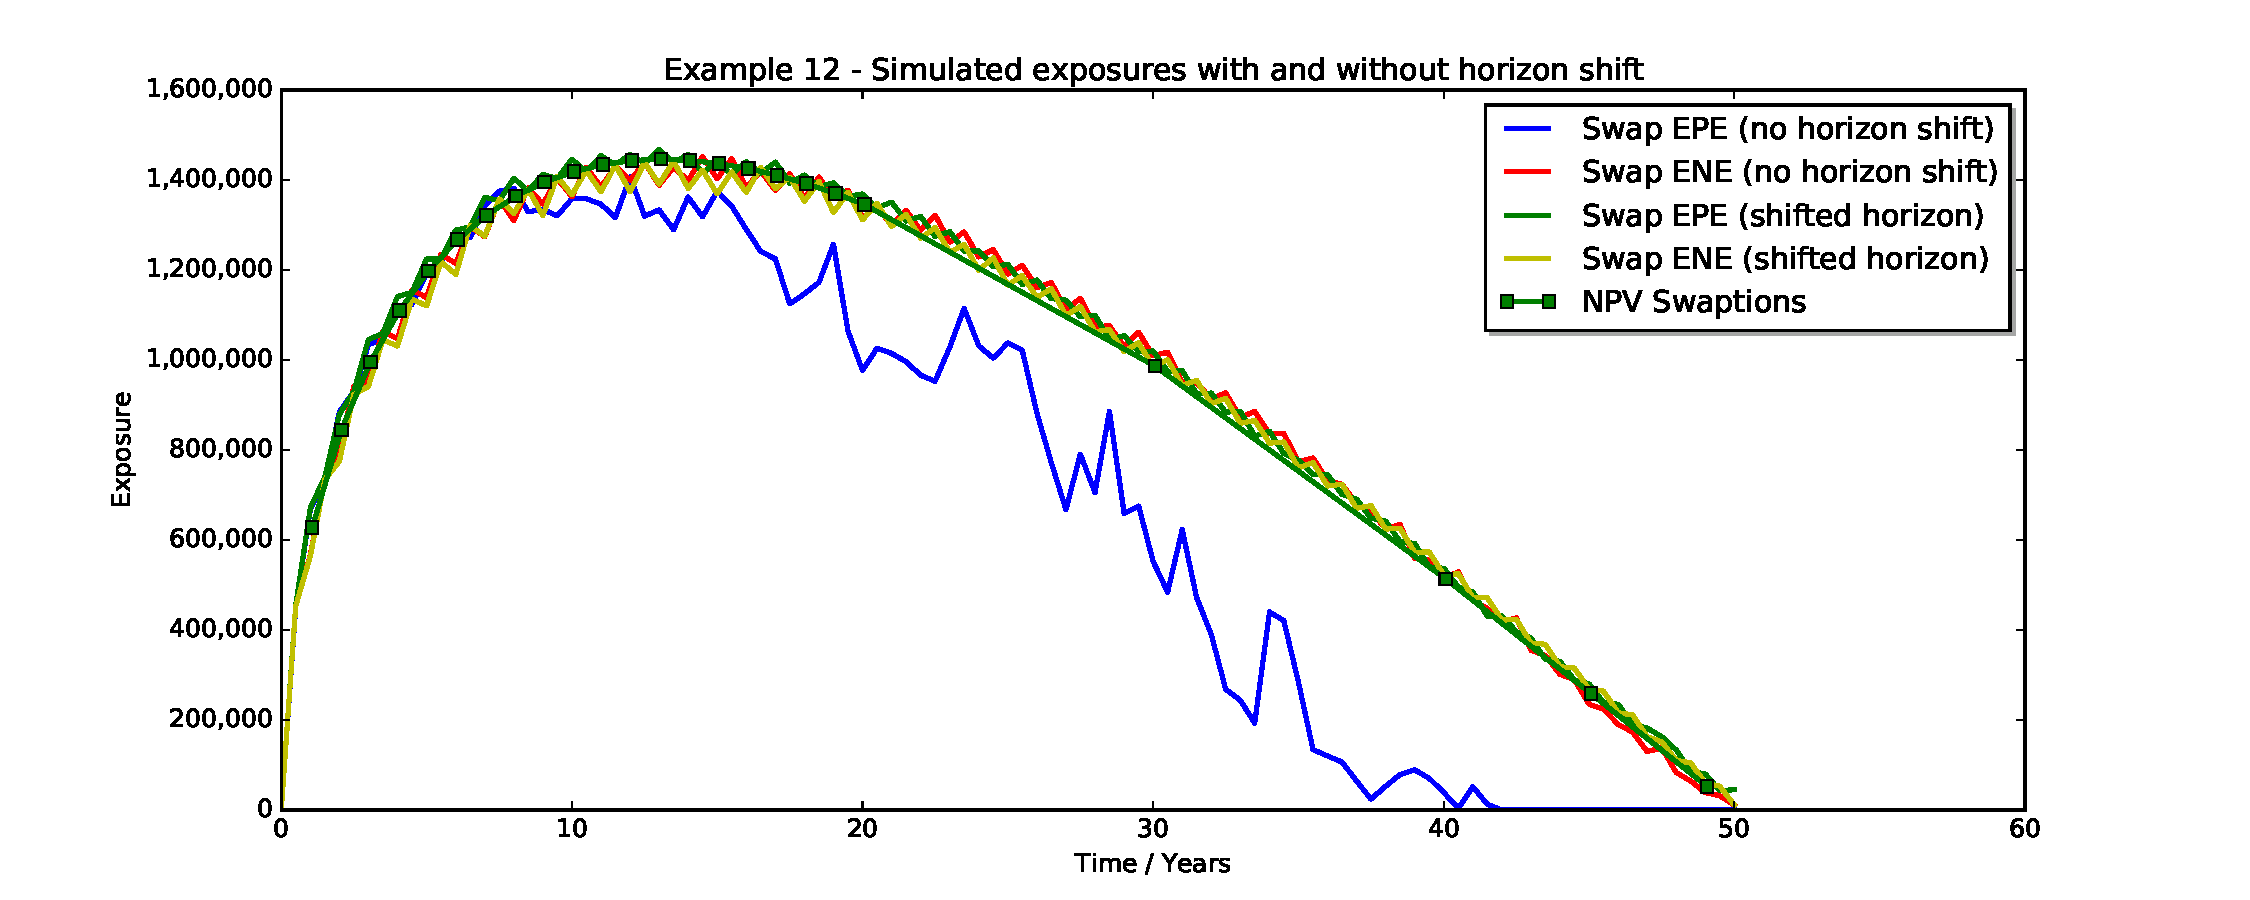
\includegraphics[scale=0.45]{examples/mpl_longterm.pdf}
\end{center}
\caption{Long term Swap exposure simulation with and without horizon shift.}
\label{fig_15}
\end{figure}
Figure \ref{fig_15b} further illustrates the origin of the problem and its resolution: The rate distribution's mean
(without horizon shift or change of measure) drifts upwards due to convexity effects (note that the yield curve is flat
in this example), and the distribution's width is then too narrow at long horizons to yield a sufficient number of low
rate scenarios with contributions to the Swap's $\EPE$ (it is a floating rate payer). With the horizon shift (change of
measure), the distribution's mean is pulled 'back' at long horizons, because the convexity effect is effectively wiped
out at the chosen horizon, and the expected rate matches the forward rate.

\begin{figure}[h!]
\begin{center}
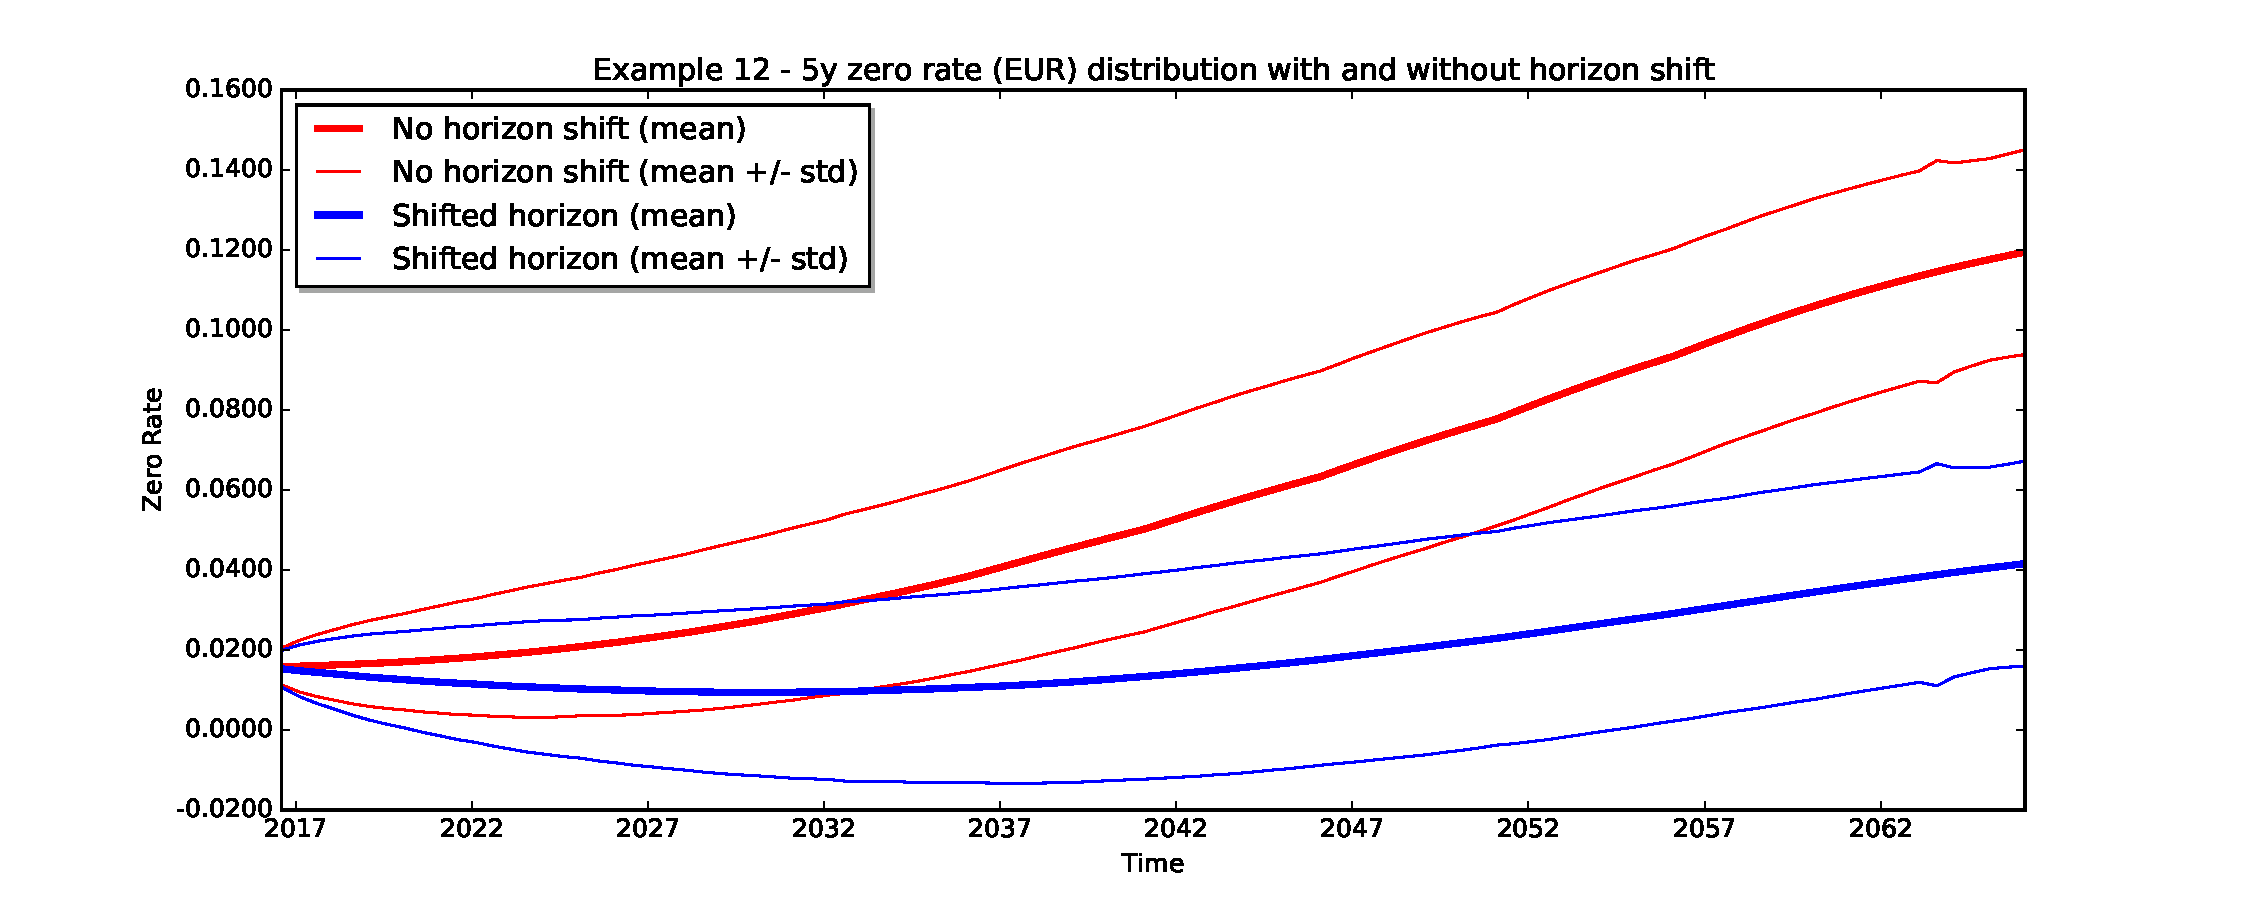
\includegraphics[scale=0.45]{examples/mpl_rates.pdf}
\end{center}
\caption{Evolution of rate distributions with and without horizon shift (change of measure). Thick lines indicate mean
  values, thin lines are contours of the rate distribution at $\pm$ one standard deviation.}
\label{fig_15b}
\end{figure}

\subsubsection{Choice of Measure}\label{example:exposure_measures}

Calling

\medskip
\centerline{\tt python run\_measures.py } 
\medskip

illustrates the effect of measure changes on simulated expected and peak exposures. For that purpose we reuse
the example in section \ref{example:exposure_swapflat} (un-collateralized vanilla swap exposure) and run the simulation
three times with different risk-neutral measures,
\begin{itemize}
\item in the LGM measure as in Example 1 (note {\tt <Measure>LGM</Measure>} in {\tt simulation\_lgm.xml}, this is the
  default also if the Measure tag is omitted)  
\item in the more common Bank Account measure (note {\tt <Measure>BA</Measure>} in {\tt simulation\_ba.xml})  
\item in the T-Forward measure with horizon T=20 at the Swap maturity (note {\tt <Measure>LGM</Measure>}  and
  {\tt <ShiftHorizon>20.0</ShiftHorizon>} in {\tt simulation\_fwd.xml})
\end{itemize}

The results are summarized in the exposure evolution graphs in figure \ref{fig:36}. As expected, the expected exposures
evolutions match across measures, as these are expected discounted NPVs and hence measure independent.
However, peak exposures are dependent on the measure choice as confirmed graphically here. Many more measures are
accessible with ORE, by way of varying the T-Forward horizon which was chosen arbitrarily here to match the Swap's maturity.

\begin{figure}[h!]
\begin{center}
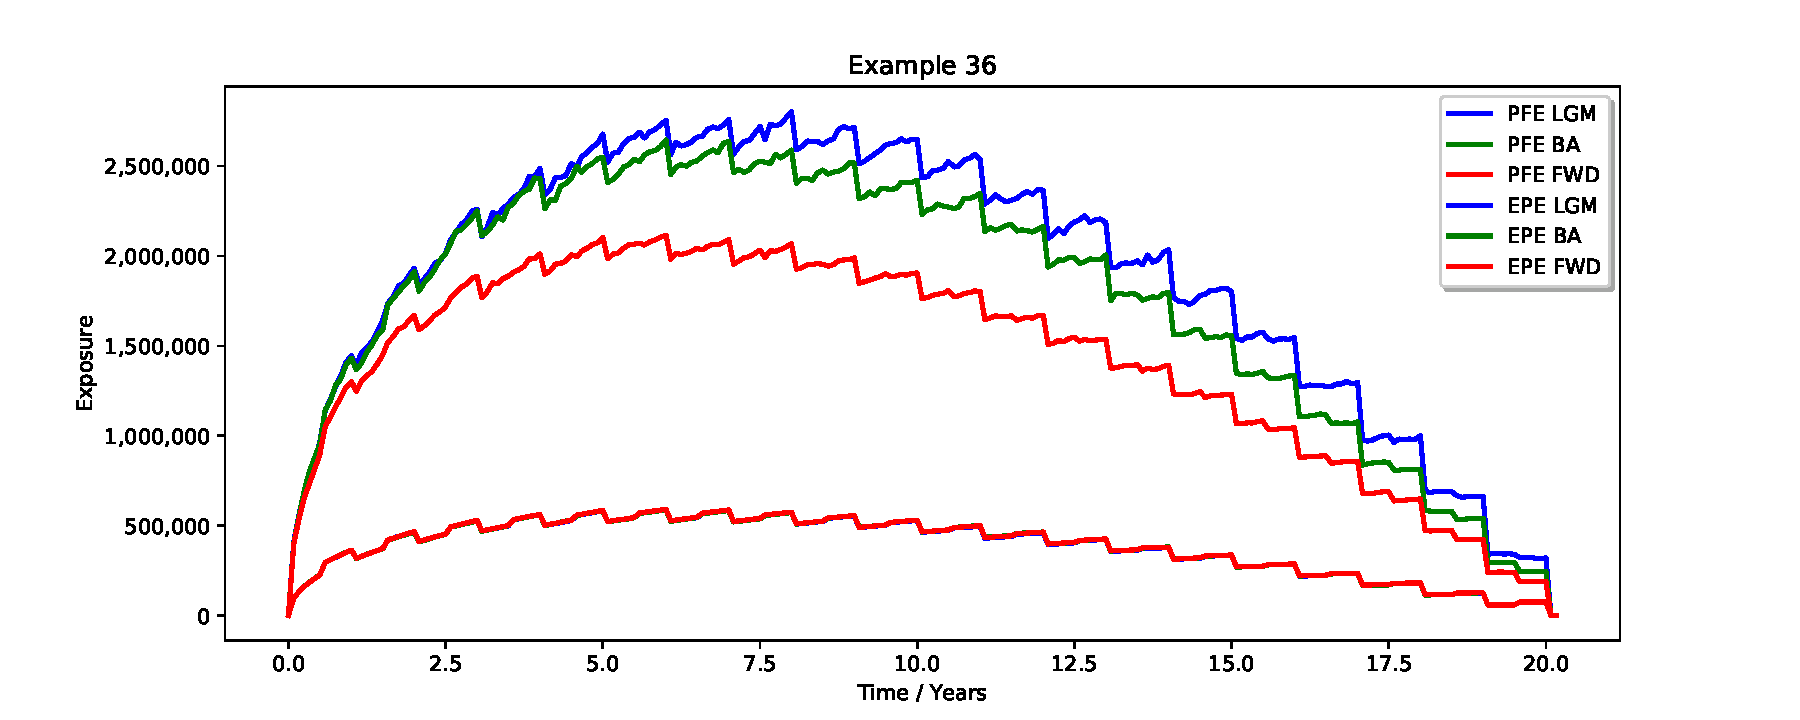
\includegraphics[scale=0.45]{examples/mpl_exposures_measures.pdf}
\end{center}
\caption{Evolution of expected exposures (EPE) and peak exposures (PFE at the 95\% quantile) in three measures, LGM,
  Bank Account, T-Forward with T=20, with 10k Monte Carlo samples.}
\label{fig:36}
\end{figure}

\subsubsection{Simulation in the two-factor Hull-White model}\label{example:exposure_hw2f}

Calling

\medskip
\centerline{\tt python run\_hw2f.py } 
\medskip

kicks off two batches, a first model calibration batch and a second exposure simulation batch.

The first batch illustrates the model calibration and scenario generation under a Hull-White multifactor
model with output in folder {\tt Examples/Exposure/Output/hw2f\_calibration}.
The model is driven by two independent Brownian motions and has four states. The diffusion matrix sigma is
therefore 2 x 4. The reversion matrix is a 4 x 4 diagonal matrix and entered as an array. Both diffusion and reversion
are constant in time. Their values are not calibrated to the option market, but hardcoded in simulation.xml.

The values for the diffusion and reversion matrices were fitted to the first two principal components of a
(hypothetical) analysis of absolute rate curve movements. These input principal components can be found in
inputeigenvectors.csv in the input folder. The tenor is given in years, and the two components are given as column
vectors, see table \ref{tab:ex37_1}.

\begin{table}[hbt]
\begin{center}
\begin{tabular}{r|r|r}
tenor & eigenvector 1  & eigenvector 2   \\
\hline      
1     & 0.353553390593 & -0.537955502871 \\
2     & 0.353553390593 & -0.374924478795 \\
3     & 0.353553390593 & -0.252916811525 \\
5     & 0.353553390593 & -0.087587539893 \\
10    & 0.353553390593 & 0.12267800393   \\
15    & 0.353553390593 & 0.240659435416  \\
20    & 0.353553390593 & 0.339148675322  \\
30    & 0.353553390593 & 0.552478951238
\end{tabular}
\caption{Input principal components}
\label{tab:ex37_1}
\end{center}
\end{table}

The first eigenvector represent perfectly parallel movements. The second eigenvector represent a rotation around the 7y
point of the curve. Furthermore we prescribe an annual volatility of 0.0070 for the first components and 0.0030 for the
second one. The values can be compared to normal (bp) volatilities.

We follow \cite{Andersen_Piterbarg_2010} chapter 12.1.5 ``Multi-Factor Statistical Gaussian Model'' to calibrate the
diffusion and reversion matrices to the prescribed components and volatilities. We do not detail the procedure here and
refer the interested reader to the given reference.

The example generates a single monte carlo path with 5000 daily steps and outputs the generated scenarios in
scenariodump.csv. The python script pca.py performs a principal component analysis on this output. The model implied
eigenvalues are given in table \ref{tab:ex37_2}.

\begin{table}[hbt]
\begin{center}
\begin{tabular}{r|r}
number & value                  \\
\hline      
1      & 4.9144936649319346e-05 \\
2      & 8.846877641067412e-06  \\
3      & 5.82566039467854e-10   \\
4      & 2.1298948225571415e-10 \\
5      & 9.254913949332787e-11  \\
6      & 1.0861256211767673e-11 \\
7      & 8.478795662698618e-14  \\
8      & 9.74468069377584e-13   \\
\end{tabular}
\caption{Input principal components}
\label{tab:ex37_2}
\end{center}
\end{table}

Only the first two values are relevant, the following are all close to zero. The square root of the first two
eigenvalues is given in table \ref{tab:ex37_3}.

\begin{table}[hbt]
\begin{center}
\begin{tabular}{r|r}
number & sqrt(value)                \\
\hline      
1      & 0.007010344973631422       \\
2      & 0.0029743701250966414      \\
\end{tabular}
\caption{Input principal components}
\label{tab:ex37_3}
\end{center}
\end{table}

matching the prescribed input values of 0.0070 and 0.0030 quite well. The corresponding eigenvectors are given in etable
\ref{tab:ex37_4}.

\begin{table}[hbt]
\begin{center}
\begin{tabular}{r|r|r}
tenor & eigenvector 1       & eigenvector 2       \\
\hline      
1     & 0.34688826736335926 & 0.5441204725042812  \\
2     & 0.3489303472083185  & 0.380259707350115   \\
3     & 0.350362134519783   & 0.2581408080614405  \\
5     & 0.3523983915961889  & 0.09230899007104967 \\
10    & 0.3550169593982022  & -0.11856777284904292\\
15    & 0.35647835947136625 & -0.23676104168229614\\
20    & 0.3577146190751303  & -0.3354486339442275 \\
30    & 0.36042236352102563 & -0.549124709243042  \\
\end{tabular}
\caption{Input principal components}
\label{tab:ex37_4}
\end{center}
\end{table}

again matching the input principal components quite well. The second eigenvector is the negative of the input vector
here (the principal component analysis can not distinguish these of course).

The example also produces a plot comparing the input eigenvectors and the model implied eigenvectors as shown in figure \ref{fig:ex37}.

\begin{figure}[h!]
\begin{center}
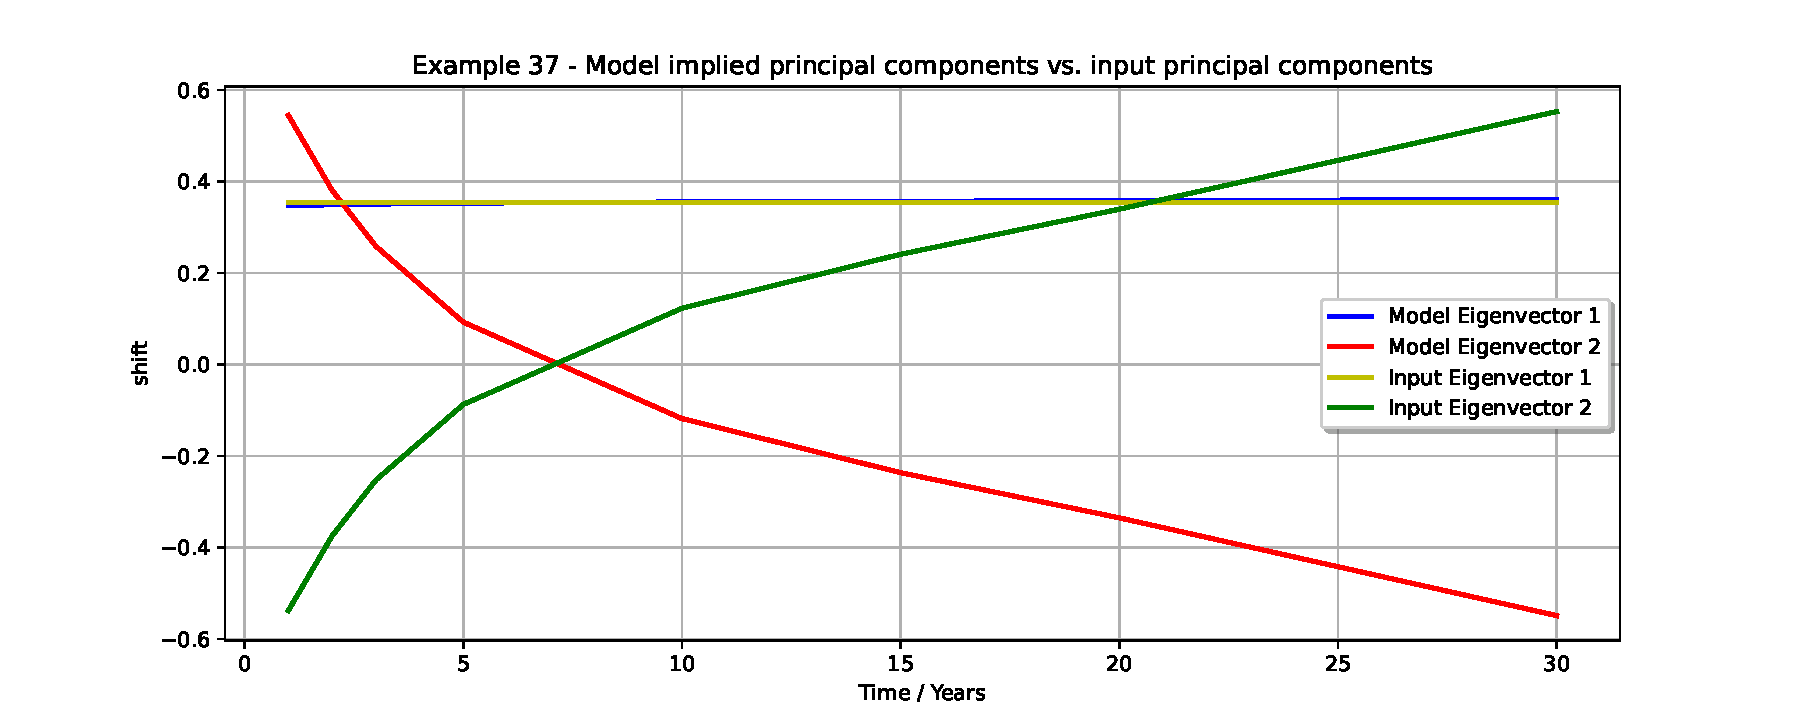
\includegraphics[scale=0.50]{examples/mpl_eigenvectors_ex37.pdf}
\end{center}
\caption{Input and model implied eigenvectors for a Hull-White 4-factor model calibrated to 2 principal components of
  rate curve movements (parallel + rotation). Notice that the model implied 2nd eigenvector is the negative of the input
  vector.}
\label{fig:ex37}
\end{figure}

The second batch is similar to the Example in section \ref{example:exposure_ccs} (EPE, ENE for a xccy swap), but uses a
multifactor HW model for EUR and USD to generate scenarios. The parametrization of the HW models is taken from the previous run,
resukts are found in folder {\tt Examples/Exposure/Output/hw2f}.

Each of the two factors of each HW model is correlated with each of the two factors of the other currency's HW model and
with the FX factors. Remember that the factors represent principal components of interest rate movements and so the
correlations can be interpreted as correlations of these principal components with each other and the fx rate processes.

\subsubsection{Wrong-Way-Risk}\label{example:exposure_wwr}

Calling

\medskip
\centerline{\tt python run\_wwr.py } 
\medskip

runs an extension of the example in section \ref{example:exposure_swapflat} (single uncollateralised Swap) with dynamic
credit and non-zero IR-CR correlation. Results are found in folder {\tt Exposure/Output/wwr}.
As we are paying float, negative correlation implies that we pay more when the counterparty's credit worsens, leading to
a surge of CVA.

The following table lists the XVA result from the example at different levels of correlation.

\begin{table}[hbt]
\scriptsize
\begin{center}
\begin{tabular}{|r|l|r|r|r|r|}
\hline
Correlation & NettingSetId & CVA & DVA & FBA & FCA \\
\hline
 -30\%  &  CPTY\_A  & 105,146  &  68,061  &  31,519  &  -4,127 \\
 -20\%  &  CPTY\_A  &  88,442  &  68,061  &  30,976  &  -4,219 \\
 -10\%  &  CPTY\_A  &  71,059  &  68,061  &  30,439  &  -4,314 \\
   0\%  &  CPTY\_A  &  52,983  &  68,061  &  29,909  &  -4,411 \\
  10\%  &  CPTY\_A  &  34,199  &  68,061  &  29,386  &  -4,511 \\
  20\%  &  CPTY\_A  &  14,691  &  68,061  &  28,869  &  -4,614 \\
  30\%  &  CPTY\_A  &  -5,554  &  68,061  &  28,360  &  -4,719 \\
\hline
\end{tabular}
\caption{IR Swap XVA results with LGM model}
\end{center}
\end{table}

\subsubsection{Flip View}\label{example:exposure_flipview}

Calling

\medskip
\centerline{\tt python run\_flipview.py } 
\medskip

demonstrates how ORE can be used to quickly switch perspectives in XVA calculations with minimal changes in the {\tt ore.xml}
file only. In particular it avoids manipulating the portfolio input or the netting set.


\subsection{Netting Set Exposure and Collateral}\label{example:exposurewithcollateral}

In this section we demonstrate exposure calculation and XVA at the level of a small netting set
consisting of three Swaps in different currencies. We ilustrate the effect of several collateral choices
on the resulting exposure.

\subsubsection{MPoR (Biweekly) Grid}

Move to folder {\tt Examples/ExposureWithCollateral}. Calling

\medskip
\centerline{\tt python run\_biweekly.py } 
\medskip

performs several calculations on a bi-weekly date grid with grid spacing that matches the Margin Period of Risk (MPoR).
The results of the related ORE runs are found in sub-directories of {\tt ExposureWithCollateral/Output/} (iah\_0, iah\_1,
nocollateral, vm\_threshold\_*, vm\_mta, vm\_mpor)

The effect of the various collateral choices is illustrated in three plots
\begin{itemize}
\item no collateral - figure \ref{fig_8},
\item collateral with threshold (THR) 1m EUR, minimum transfer amount (MTA) 100k EUR, margin period of risk (MPOR) 2
  weeks - figure \ref{fig_9}
\item collateral with zero THR and MTA, and MPOR 2w - figure \ref{fig_10}
\end{itemize}
The exposure graphs with collateral and positive margin period of risk show typical spikes. What is causing these? As
sketched in \cite{methods}, ORE uses a {\em classical collateral model} that applies collateral
amounts to offset exposure with a time delay that corresponds to the margin period of risk. The spikes are then caused
by instrument cash flows falling between exposure measurement dates $d_1$ and $d_2$ (an MPOR apart), so that a
collateral delivery amount determined at $d_1$ but settled at $d_2$ differs significantly from the closeout amount at
$d_2$ causing a significant residual exposure for a short period of time. See for example \cite{Andersen2016} for a
recent detailed discussion of collateral modelling. The approach currently implemented in ORE corresponds to {\em
  Classical+} in \cite{Andersen2016}, the more conservative approach of the classical methods. The less conservative
alternative, {\em Classical-}, would assume that both parties stop paying trade flows at the beginning of the MPOR, so
that the P\&L over the MPOR does not contain the cash flow effect, and exposure spikes are avoided. Note that the size
and position of the largest spike in figure \ref{fig_9} is consistent with a cash flow of the 40 million GBP Swap in the
example's portfolio that rolls over the 3rd of March and has a cash flow on 3 March 2020, a bit more than four years
from the evaluation date.
  
\begin{figure}[h!]
\begin{center}
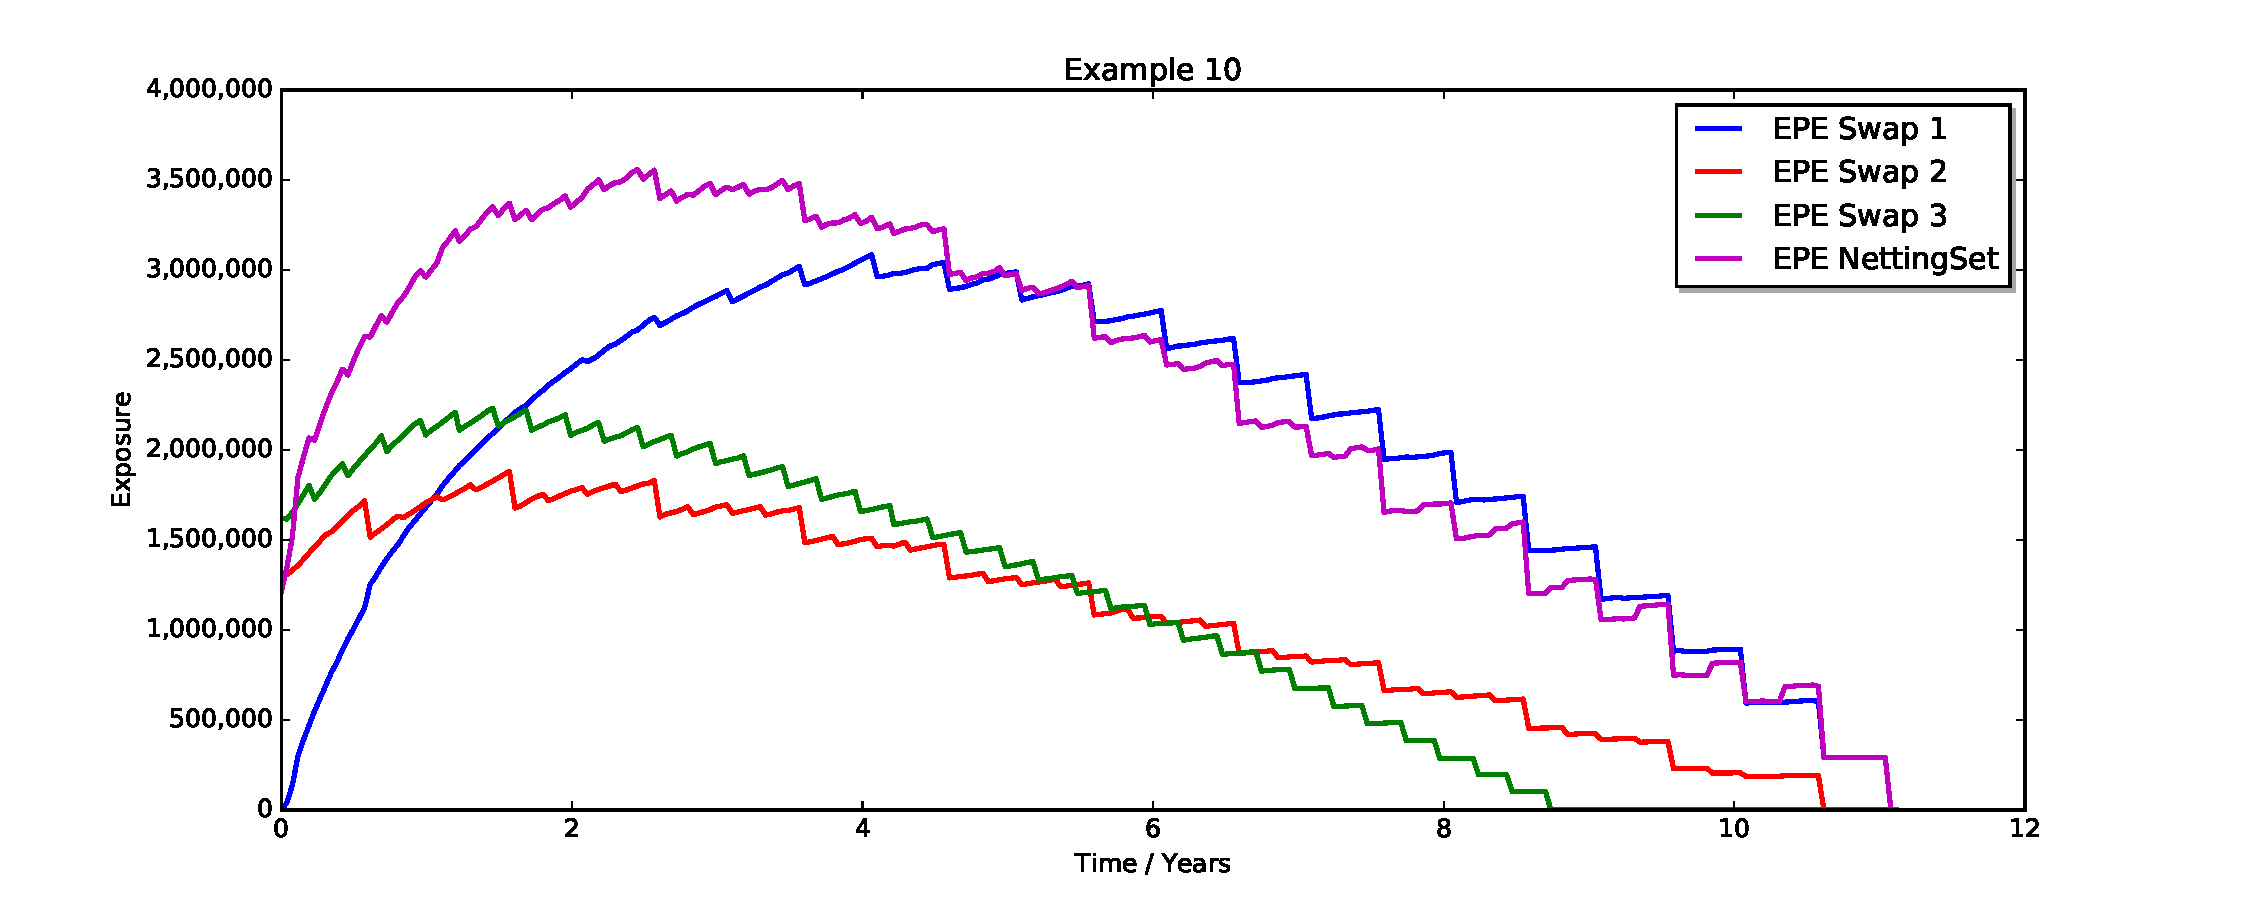
\includegraphics[scale=0.45]{examples/mpl_nocollateral_epe.pdf}
\end{center}
\caption{Three Swaps netting set, no collateral. Simulation with 5000 paths and bi-weekly time steps.}
\label{fig_8}
\end{figure}

\begin{figure}[htb]
\begin{center}
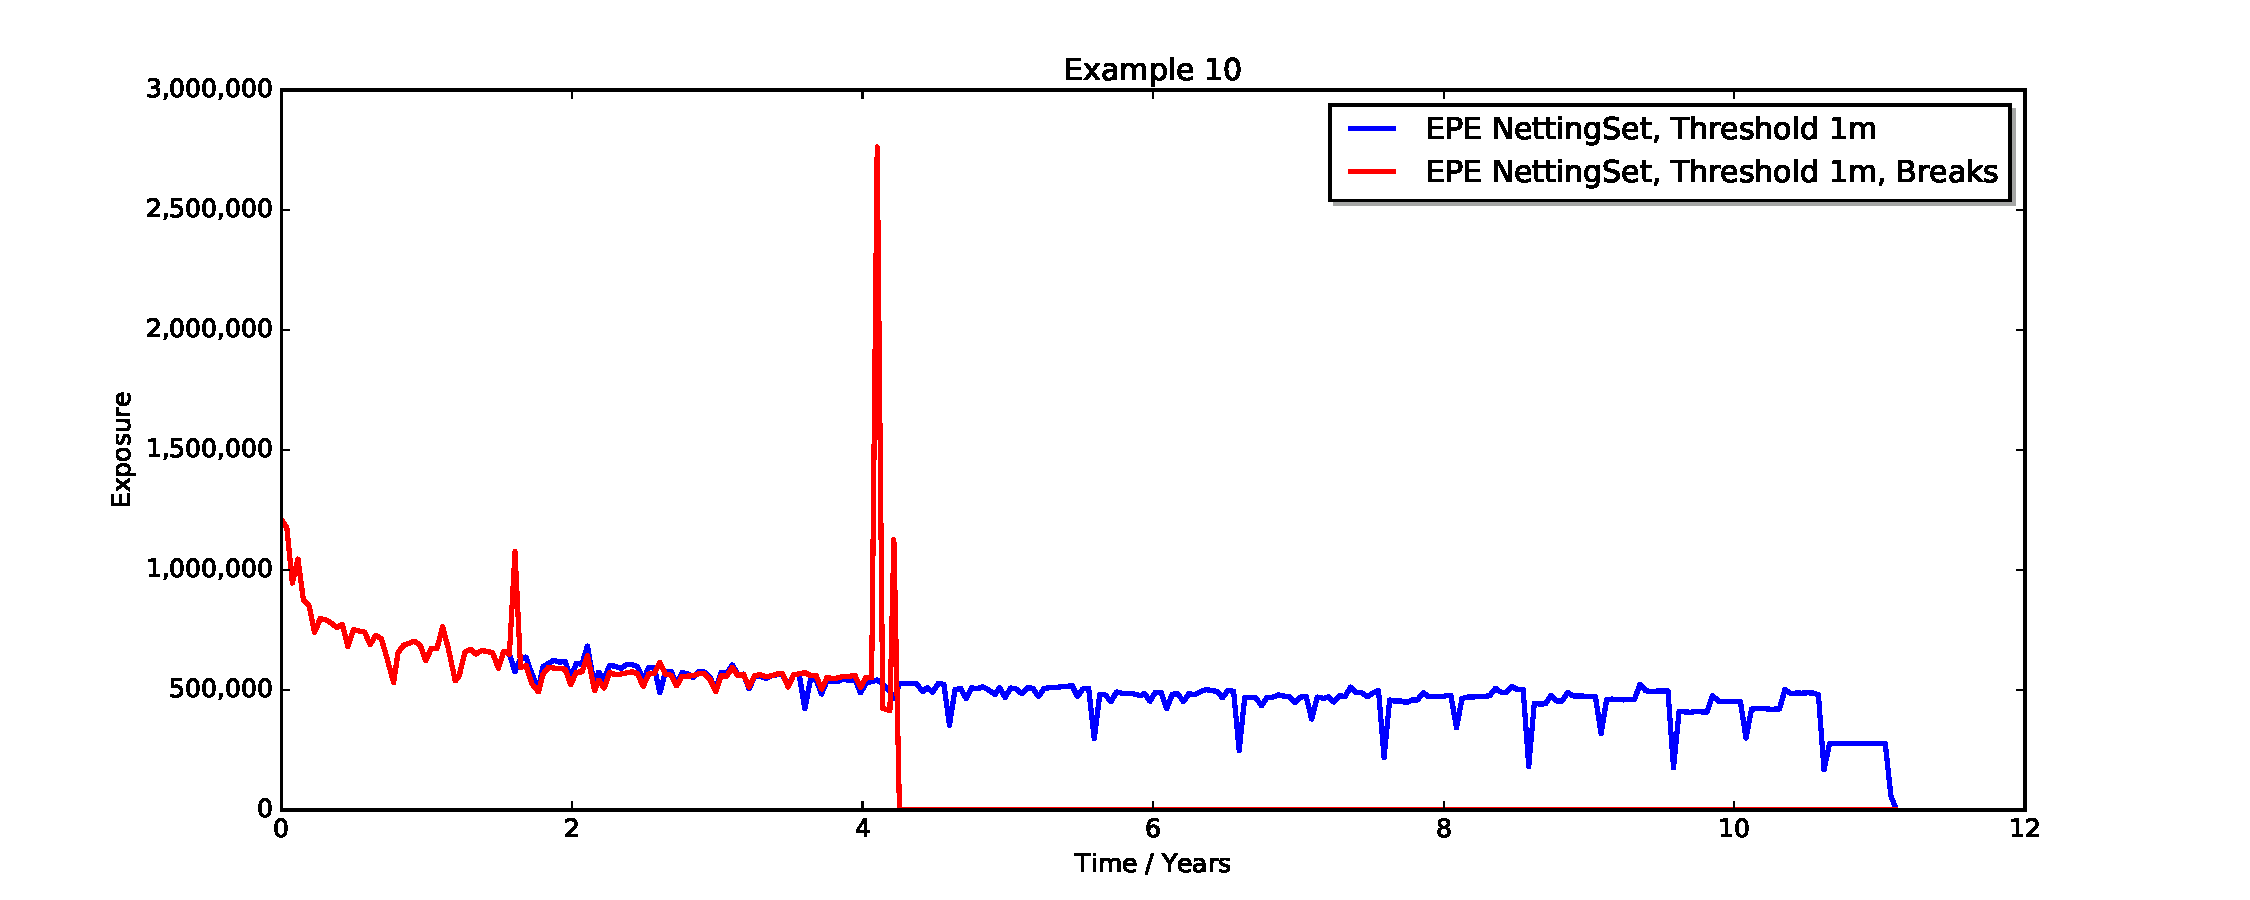
\includegraphics[scale=0.45]{examples/mpl_threshold_break_epe.pdf}
\end{center}
\caption{Three Swaps netting set, THR=1m EUR, MTA=100k EUR, MPOR=2w. The red evolution assumes that the each trade is
  terminated at the next break date. The blue evolution ignores break dates. Simulation with 5000 paths and bi-weekly
  time steps.}
\label{fig_9}
\end{figure}

%\begin{figure}[h]
%\begin{center}
%\includegraphics[scale=1.0]{example_mta_epe.pdf}
%\end{center}
%\caption{Three swaps, threshold = 0, mta > 0.}
%\label{fig_7}
%\end{figure}

\begin{figure}[h!]
\begin{center}
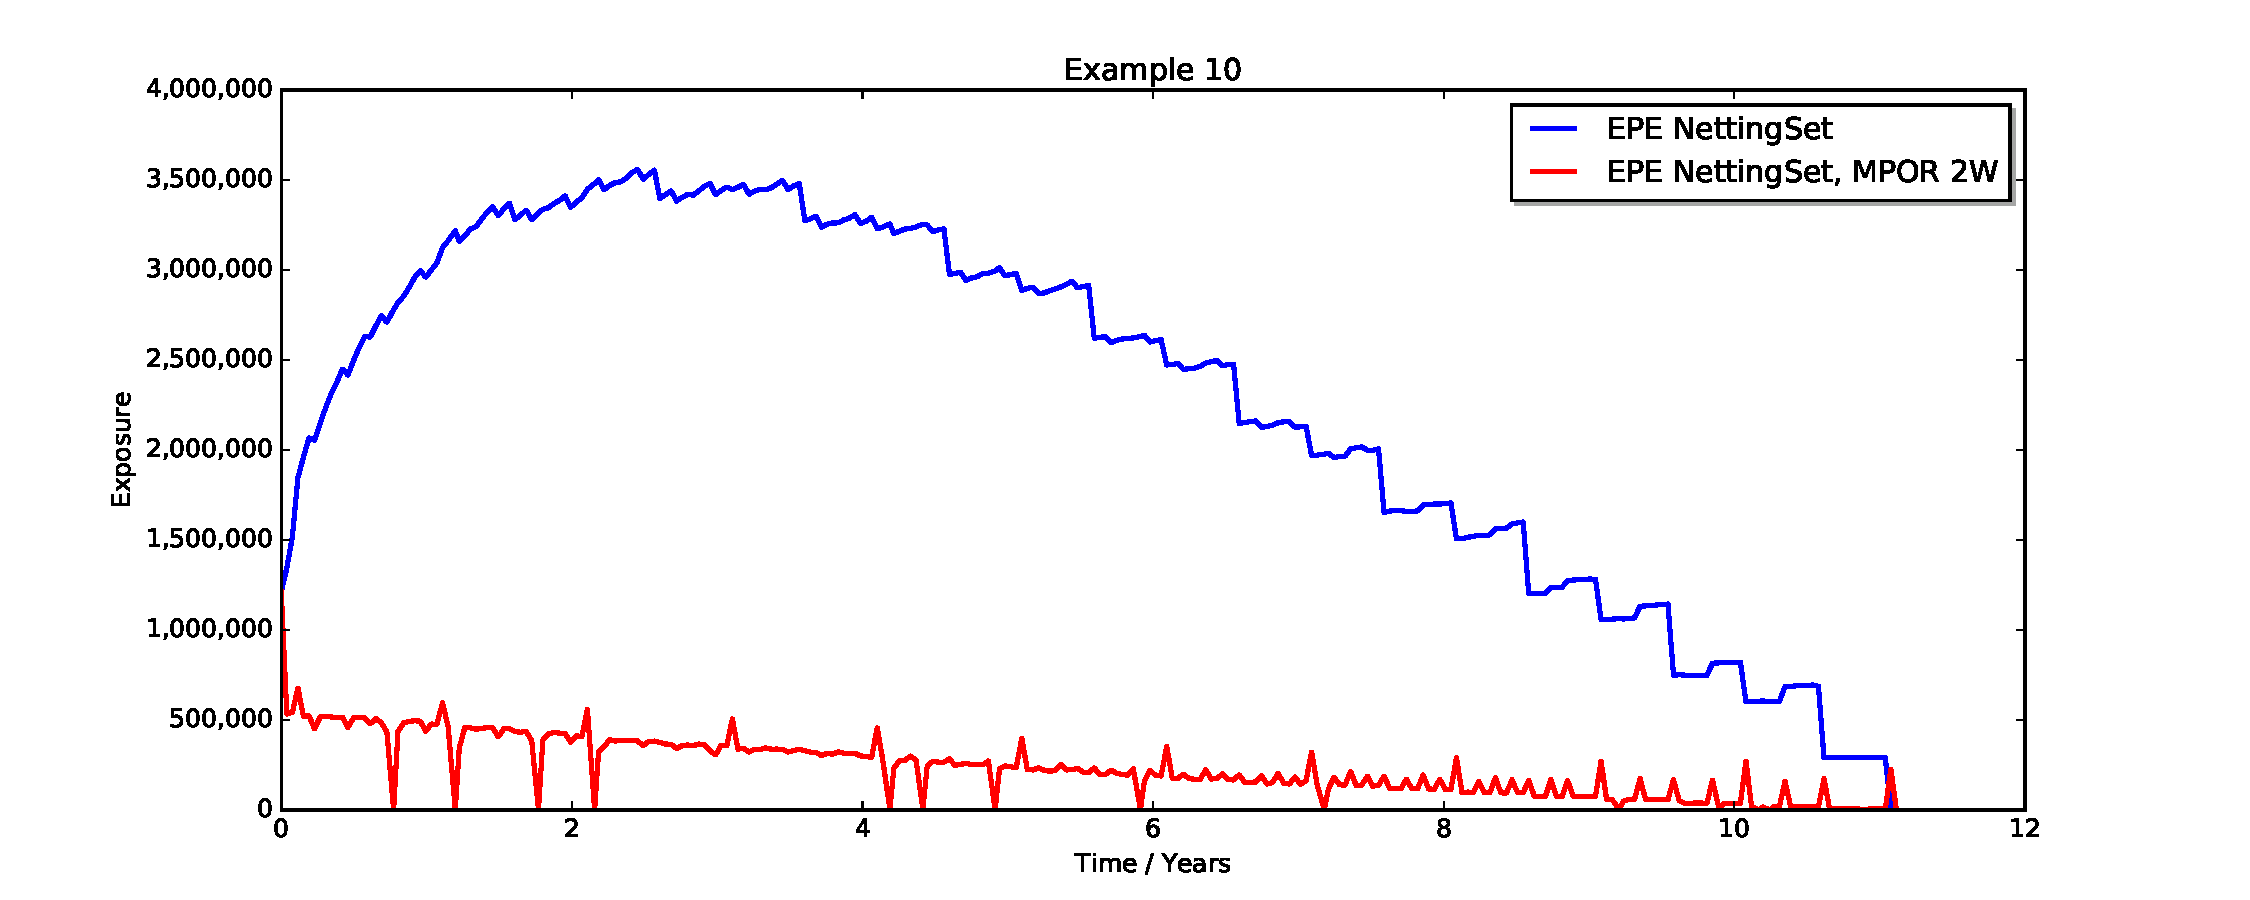
\includegraphics[scale=0.45]{examples/mpl_mpor_epe.pdf}
\end{center}
\caption{Three Swaps, THR=MTA=0, MPOR=2w. Simulation with 5000 paths and bi-weekly time steps.}
\label{fig_10}
\end{figure}


\subsubsection*{CVA, DVA, FVA, COLVA, MVA, Collateral Floor}

We use one of the cases to demonstrate the XVA outputs, see folder {\tt Examples/ExposureWithCollateral/Output/vm\_threshold\_dim}.

\medskip The summary of all value adjustments (CVA, DVA, FVA, COLVA, MVA, as well as the Collateral Floor) is provided
in file {\tt xva.csv}.  The file includes the allocated CVA and DVA numbers to individual trades as introduced in the
next section. The following table illustrates the file's layout, omitting the three columns containing allocated data.

\begin{center}
\resizebox{\columnwidth}{!}{%
\begin{tabular}{|l|l|r|r|r|r|r|r|r|r|r|}
\hline
TradeId & NettingSetId & CVA & DVA & FBA & FCA & COLVA & MVA & CollateralFloor & BaselEPE & BaselEEPE \\
\hline
 & CPTY\_A &  6,521  &  151,193  & -946  &  72,103  &  2,769  & -14,203  &  189,936  &  113,260  &  1,211,770 \\
Swap\_1 & CPTY\_A &  127,688  &  211,936  & -19,624  &  100,584  &  n/a  &  n/a  &  n/a   &  2,022,590  &  2,727,010 \\
Swap\_3 & CPTY\_A &  71,315  &  91,222  & -11,270  &  43,370  &  n/a  &  n/a  &  n/a   &  1,403,320  &  2,183,860 \\
Swap\_2 & CPTY\_A &  68,763  &  100,347  & -10,755  &  47,311  &  n/a  &  n/a  &  n/a   &  1,126,520  &  1,839,590 \\
\hline
\end{tabular}
}
\end{center}

The line(s) with empty TradeId column contain values at netting set level, the others contain uncollateralised
single-trade VAs.  Note that COLVA, MVA and Collateral Floor are only available at netting set level at which collateral
is posted.

\medskip
Detailed output is written for COLVA and Collateral Floor to file {\tt colva\_nettingset\_*.csv} which shows the 
incremental contributions to these two VAs through time.


\subsubsection*{Exposure Reports \& XVA Allocation to Trades}

We also illustrate here the layout of an exposure report produced by ORE. The report shows the exposure evolution of
Swap\_1 without collateral which is found in folder \\
{\tt Examples/ExposureWithCollateral/Output/nocollateral/exposure\_trade\_Swap\_1.csv}:

\begin{center}
\resizebox{\columnwidth}{!}{%
\begin{tabular}{|l|l|r|r|r|r|r|r|r|r|}
\hline
TradeId & Date & Time & EPE & ENE & AllocEPE & AllocENE & PFE & BaselEE & BaselEEE \\
\hline
Swap\_1 & 05/02/16 & 0.0000 & 0  & 1,711,748  & 0  & 0  & 0  & 0  & 0 \\
Swap\_1 & 19/02/16 & 0.0383 & 38,203   & 1,749,913  & -1,200,677 & 511,033 & 239,504 & 38,202 & 38,202 \\
Swap\_1 & 04/03/16 & 0.0765 & 132,862  & 1,843,837 & -927,499 & 783,476 & 1,021,715 & 132,845 & 132,845 \\
%Swap\_1 & 18/03/16 & 0.1148 & 299,155  & 1,742,450  & -650,225  & 793,067  & 1,914,150  & 299,091  & 299,091 \\
%Swap\_1 & 01/04/16 & 0.1530 & 390,178  & 1,834,810  & -552,029  & 892,604  & 2,373,560  & 390,058  & 390,058 \\
%Swap\_1 & 15/04/16 & 0.1913 & 471,849  & 1,918,600  & -465,580  & 981,171  & 2,765,710  & 471,659  & 471,659 \\
%Swap\_1 & 29/04/16 & 0.2295 & 550,301  & 2,000,640  & -330,578  & 1,119,760  & 3,106,810  & 550,016  & 550,016 \\
%Swap\_1 & 13/05/16 & 0.2678 & 620,279  & 2,074,880  & -266,042  & 1,188,560  & 3,427,080  & 619,888  & 619,888 \\
%Swap\_1 & 27/05/16 & 0.3060 & 690,018  & 2,140,320  & -190,419  & 1,259,880  & 3,778,570  & 689,509  & 689,509 \\
%Swap\_1 & 10/06/16 & 0.3443 & 763,207  & 2,206,020  & -137,681  & 1,305,130  & 4,052,870  & 762,560  & 762,560 \\
Swap\_1 & ... & ...& ... & ... & ... & ... & ... & ... & ... \\
\hline
\end{tabular}
}
\end{center}

The exposure measures EPE, ENE and PFE, the Basel exposure measures $EE_B$ and $EEE_B$, as well as allocated exposures
are defined in \cite{methods}. The PFE quantile and allocation method are chosen as described in section \ref{sec:analytics}. \\

In addition to single trade exposure files, ORE produces an exposure file per netting set. The example from the same
folder as above is:

\begin{center}
\resizebox{\columnwidth}{!}{%
\begin{tabular}{|l|l|r|r|r|r|r|r|r|}
\hline
NettingSet & Date & Time & EPE & ENE & PFE & ExpectedCollateral & BaselEE & BaselEEE \\
\hline
CPTY\_A & 05/02/16 & 0.0000 & 1,203,836 & 0 & 1,203,836 & 0 & 1,203,836 & 1,203,836 \\%1,211,770 & 0 & 1,211,770 & 0 & 1,211,770 & 1,211,770\\
CPTY\_A & 19/02/16 & 0.0383 & 1,337,713 & 137,326 & 3,403,460 & 0 & 1,337,651 & 1,337,651 \\ %0.0383 & 1,344,220 & 137,776 & 3,414,000 & 0 & 1,344,160 & 1,344,160\\
%CPTY\_A & 04/03/16 & 0.0765 & 1,518,610 & 308,381 & 4,354,060 & 0 & 1,518,410 & 1,518,410\\
%CPTY\_A & 18/03/16 & 0.1148 & 1,846,900 & 382,068 & 5,200,730 & 0 & 1,846,500 & 1,846,500\\
%CPTY\_A & 01/04/16 & 0.1530 & 1,961,290 & 494,416 & 5,869,470 & 0 & 1,960,690 & 1,960,690\\
%CPTY\_A & 15/04/16 & 0.1913 & 2,067,240 & 598,283 & 6,384,140 & 0 & 2,066,400 & 2,066,400\\
%CPTY\_A & 29/04/16 & 0.2295 & 2,053,670 & 745,960 & 6,740,070 & 0 & 2,052,610 & 2,066,400\\
%CPTY\_A & 13/05/16 & 0.2678 & 2,149,190 & 845,507 & 6,930,230 & 0 & 2,147,840 & 2,147,840\\
%CPTY\_A & 27/05/16 & 0.3060 & 2,235,630 & 930,218 & 7,295,440 & 0 & 2,233,980 & 2,233,980\\
%CPTY\_A & 10/06/16 & 0.3443 & 2,314,470 & 1,014,690 & 7,753,190 & 0 & 2,312,510 & 2,312,510\\
CPTY\_A & ... & ...& ... & ... & ... & ... & ... & ...\\
%CPTY\_A & 07/07/17 & 1.4167 & 3,320,430 & 2,423,890 & 12,787,900 & 0 & 3,304,650 & 3,304,650\\
%CPTY\_A & 21/07/17 & 1.4551 & 3,351,780 & 2,452,640 & 12,964,200 & 0 & 3,335,420 & 3,335,420\\
%CPTY\_A & 04/08/17 & 1.4934 & 3,302,820 & 2,511,500 & 12,796,100 & 0 & 3,286,260 & 3,335,420\\
%CPTY\_A & 18/08/17 & 1.5318 & 3,339,840 & 2,545,850 & 13,120,000 & 0 & 3,322,640 & 3,335,420\\
%CPTY\_A & 01/09/17 & 1.5701 & 3,371,300 & 2,576,100 & 13,238,700 & 0 & 3,353,480 & 3,353,480\\
%CPTY\_A & 15/09/17 & 1.6085 & 3,279,670 & 2,555,370 & 13,041,300 & 0 & 3,261,880 & 3,353,480\\
%CPTY\_A & 29/09/17 & 1.6468 & 3,305,060 & 2,579,200 & 13,072,800 & 0 & 3,286,680 & 3,353,480\\
%CPTY\_A & 13/10/17 & 1.6852 & 3,332,830 & 2,604,200 & 13,225,600 & 0 & 3,313,850 & 3,353,480\\
%CPTY\_A & 27/10/17 & 1.7236 & 3,280,280 & 2,661,770 & 13,034,600 & 0 & 3,261,150 & 3,353,480\\
%CPTY\_A & 13/11/17 & 1.7701 & 3,316,800 & 2,701,060 & 13,331,600 & 0 & 3,296,880 & 3,353,480\\
%CPTY\_A & 24/11/17 & 1.8003 & 3,337,760 & 2,720,870 & 13,402,400 & 0 & 3,317,280 & 3,353,480\\
%CPTY\_A & ... & ...& ... & ... & ... & ... & ... & ...\\
\hline
\end{tabular}
}
\end{center}

Allocated exposures are missing here, as they make sense at the trade level only, and the expected collateral balance is
added for information (in this case zero as collateralisation is deactivated in this example).

\medskip The allocation of netting set exposure and XVA to the trade level is frequently required by finance
departments. This allocation is also featured here. We start again with the uncollateralised
case in figure \ref{fig_12}, followed by the case with threshold 1m EUR in figure \ref{fig_13}.
\begin{figure}[h!]
\begin{center}
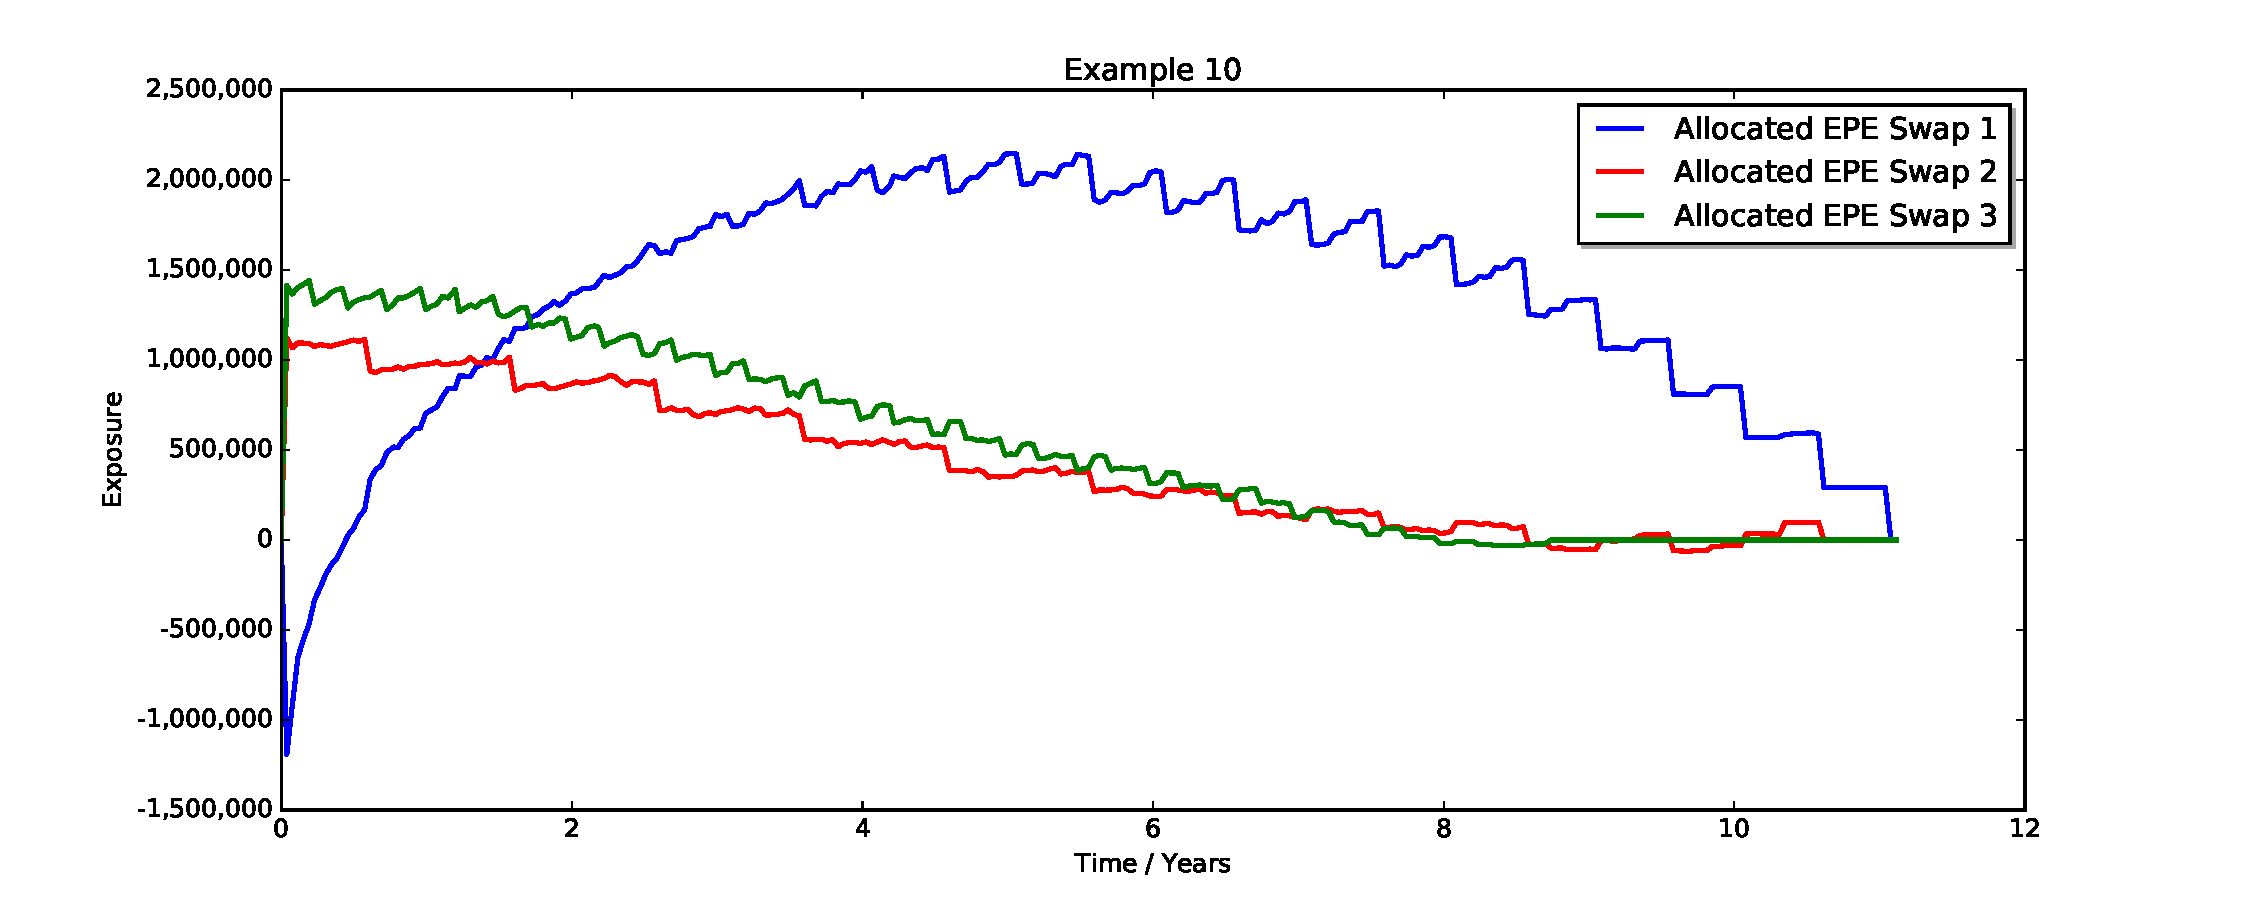
\includegraphics[scale=0.45]{examples/mpl_nocollateral_allocated_epe.pdf}
\end{center}
\caption{Exposure allocation without collateral. Simulation with 5000 paths and bi-weekly time steps.}
\label{fig_12}
\end{figure}
In both cases we apply the {\em marginal} (Euler) allocation method as published by Pykhtin and Rosen in 2010, hence we
see the typical negative EPE for one of the trades at times when it reduces the netting set exposure. The case with
collateral moreover shows the typical spikes in the allocated exposures.
\begin{figure}[h!]
\begin{center}
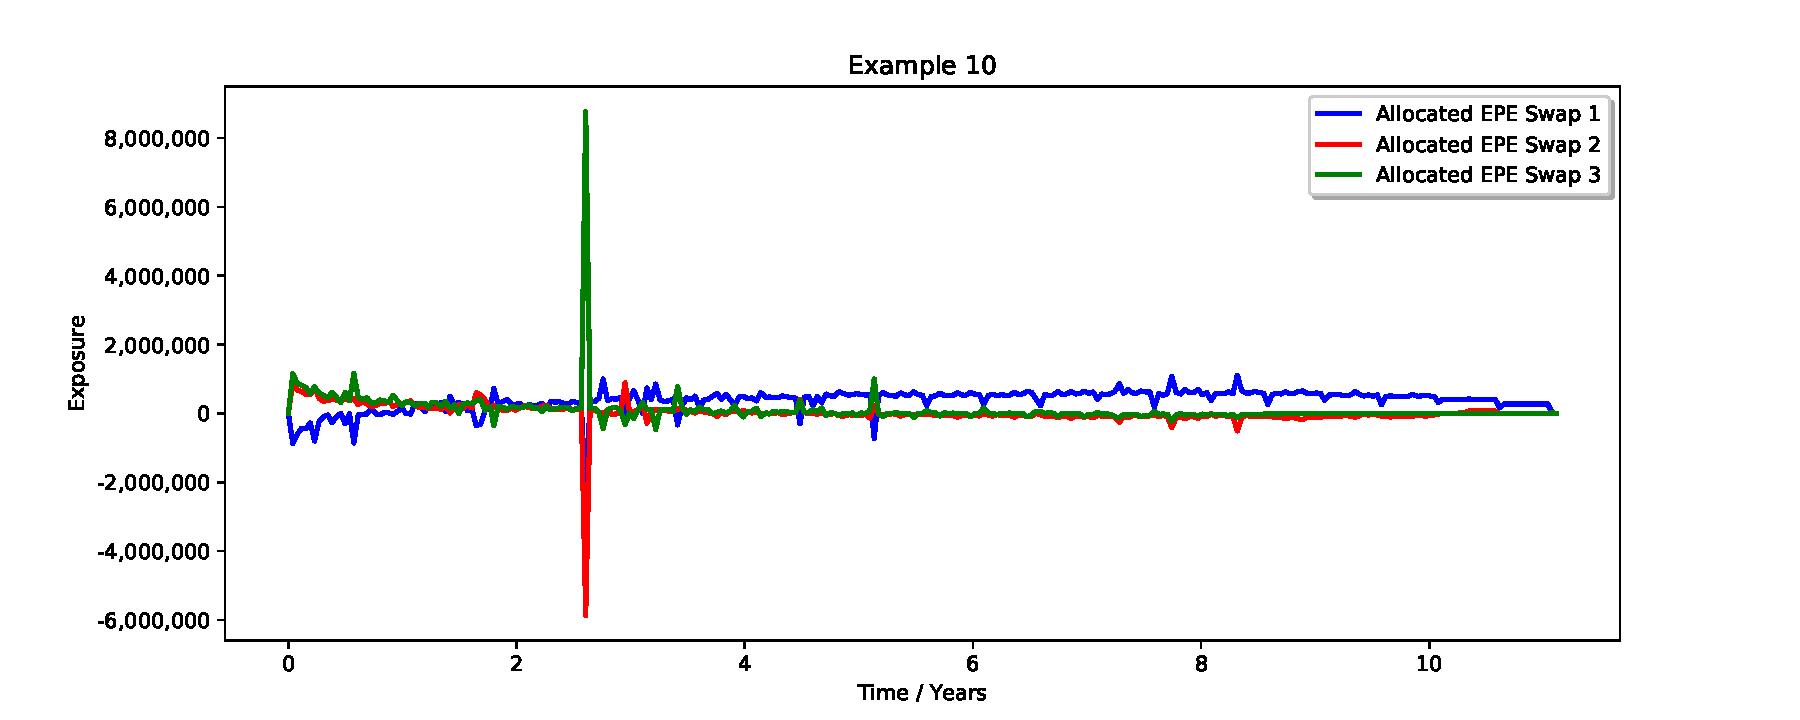
\includegraphics[scale=0.45]{examples/mpl_threshold_allocated_epe.pdf}
\end{center}
\caption{Exposure allocation with collateral and threshold 1m EUR. Simulation with 5000 paths and bi-weekly time steps.}
\label{fig_13}
\end{figure}
The analytics results also feature allocated XVAs in file {\tt xva.csv} which are derived from the allocated exposure
profiles. Note that ORE also offers alternative allocation methods to the marginal method by Pykhtin/Rosen, which can be
explored by modifying this Example.


\subsubsection{Close-out Grid}

So far  we have used a ``lagged'' collateral approach, described at the end of the collateral section in \cite{methods},
to take the Margin Period of Risk into account in exposure modelling. This used to have the disadvantage in ORE that we need
to use equally-spaced time grids with time steps that match the MPoR, e.g. 2W, out to final portfolio maturity. 

Calling

\medskip
\centerline{\tt python run\_closeout.py } 
\medskip

we demonstrate an alternative approach supported by ORE since release 6, with results in folders
{\tt ExposureWithCollateral/Output/closeout\_*}. In this approach we use two nested grids:
The (almost) arbitrary main simulation grid is used to compute ``default values'' which feed into the collateral
balance $C(t)$ filtered by MTA and Threshold etc; an auxiliary ``close-out'' grid, offset from the main grid by the MPoR,
is used to compute the delayed close-out values $V(t)$ associated with time default time $t$. The difference between $V(t)$
and $C(t)$ causes a residual exposure $[V(t)-C(t)]^+$ even if minimum transfer amounts and thresholds are zero.

The close-out date value can be computed in two ways in ORE
\begin{itemize}
\item as of default date, by just evolving the market from default date to close-out date
   (``sticky date''), or 
\item  as of close-out date, by evolving both valuation date and market over the 
   close-out period (``actual date''), i.e., the portfolio ages and cash flows might occur
   in the close-out period causing spikes in the evolution of exposures. 
\end{itemize}

We are reusing one case from Example 10 here, perfect CSA with zero threshold and
minimum transfer amount, so that the remaining exposure is solely due to the MPoR
effect. The portfolio consists of a single at-the-money Swap in GBP. 
The relevant configuration changes that trigger this modelling are in the Parameters section of {\tt simulation.xml} as shown in Listing \ref{lst:close_out_grid}

\begin{listing}[H]
\begin{minted}[fontsize=\footnotesize]{xml}
  <Parameters>
    <Grid> ... </Grid>
    <Calendar> ... </Calendar>
    <Sequence> ... </Sequence>
    <Scenario> ... </Scenario>
    <Seed> ... </Seed>
    <Samples> ... </Samples>
    <CloseOutLag> 2W </CloseOutLag>
    <MporMode> StickyDate </MporMode><!-- Alternative: ActualDate -->
  </Parameters>
\end{minted}
\caption{Close-out grid specification: Simulation parameters}
\label{lst:close_out_grid}
\end{listing}

and moreover in the XVA analytics section of {\tt ore\_mpor.xml} as shown in Listing \ref{lst:calctype_nolag}.

\begin{listing}[H]
\begin{minted}[fontsize=\footnotesize]{xml}
  <Analytic type="xva">
    ...
    <Parameter name="calculationType"> NoLag </Parameter>
    ...
  </Parameters>
\end{minted}
\caption{Close-out grid specification: XVA analytic}
\label{lst:calctype_nolag}
\end{listing}

\begin{figure}[h!]
\begin{center}
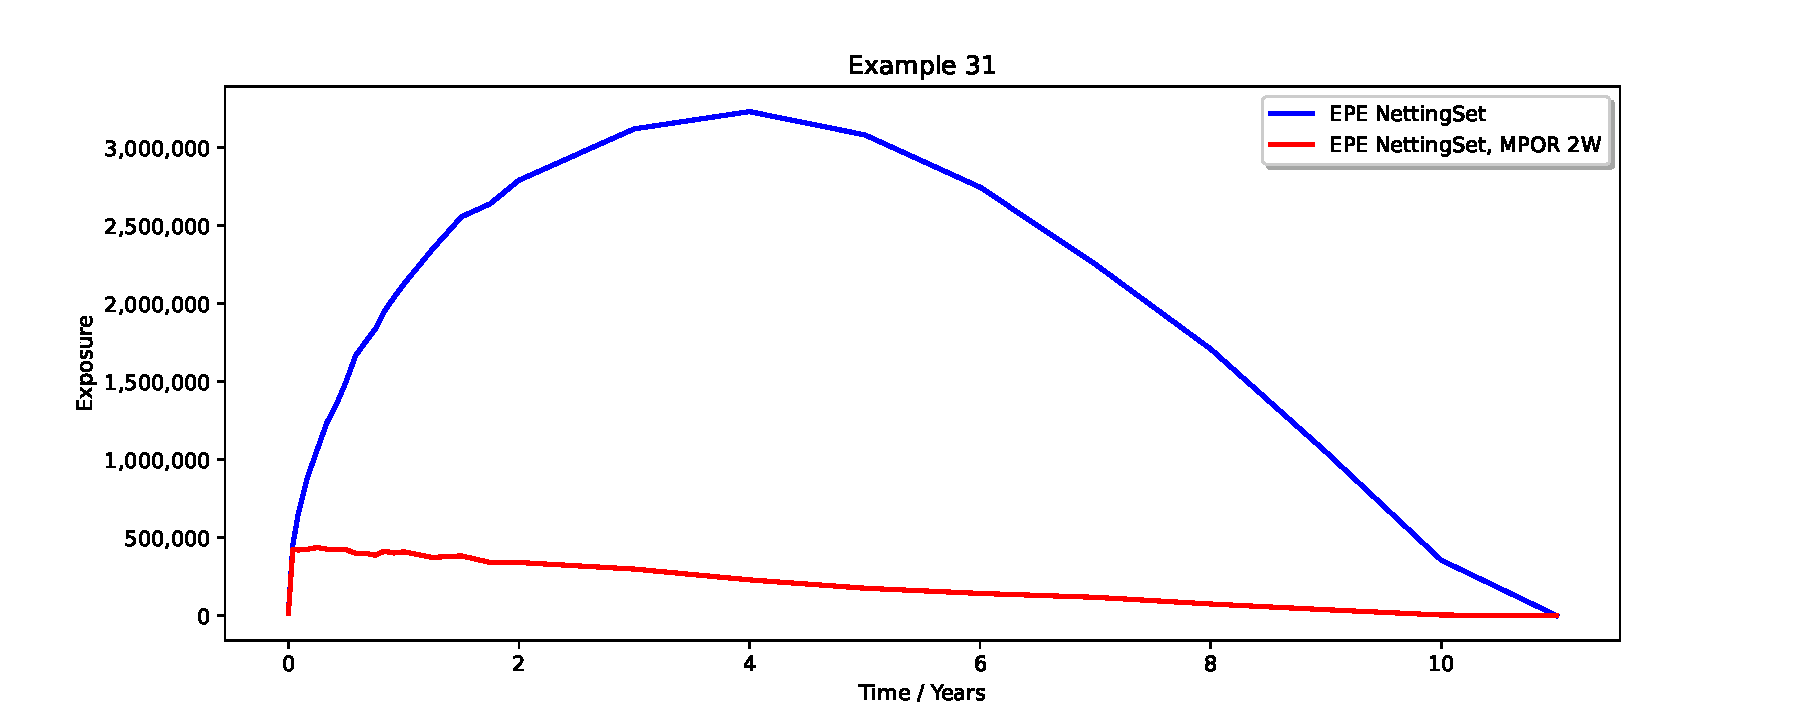
\includegraphics[scale=0.45]{examples/mpl_closeout_mpor_epe.pdf}
\end{center}
\caption{Uncollateralized Swap exposure vs exposure with Variation Margin, zero threshold and MTA.
  The simulation uses a variable grid with an auxiliary grid for closeout value calculation which is offset by the MPOR.}
\label{fig_31_a}
\end{figure}

\begin{figure}[h!]
\begin{center}
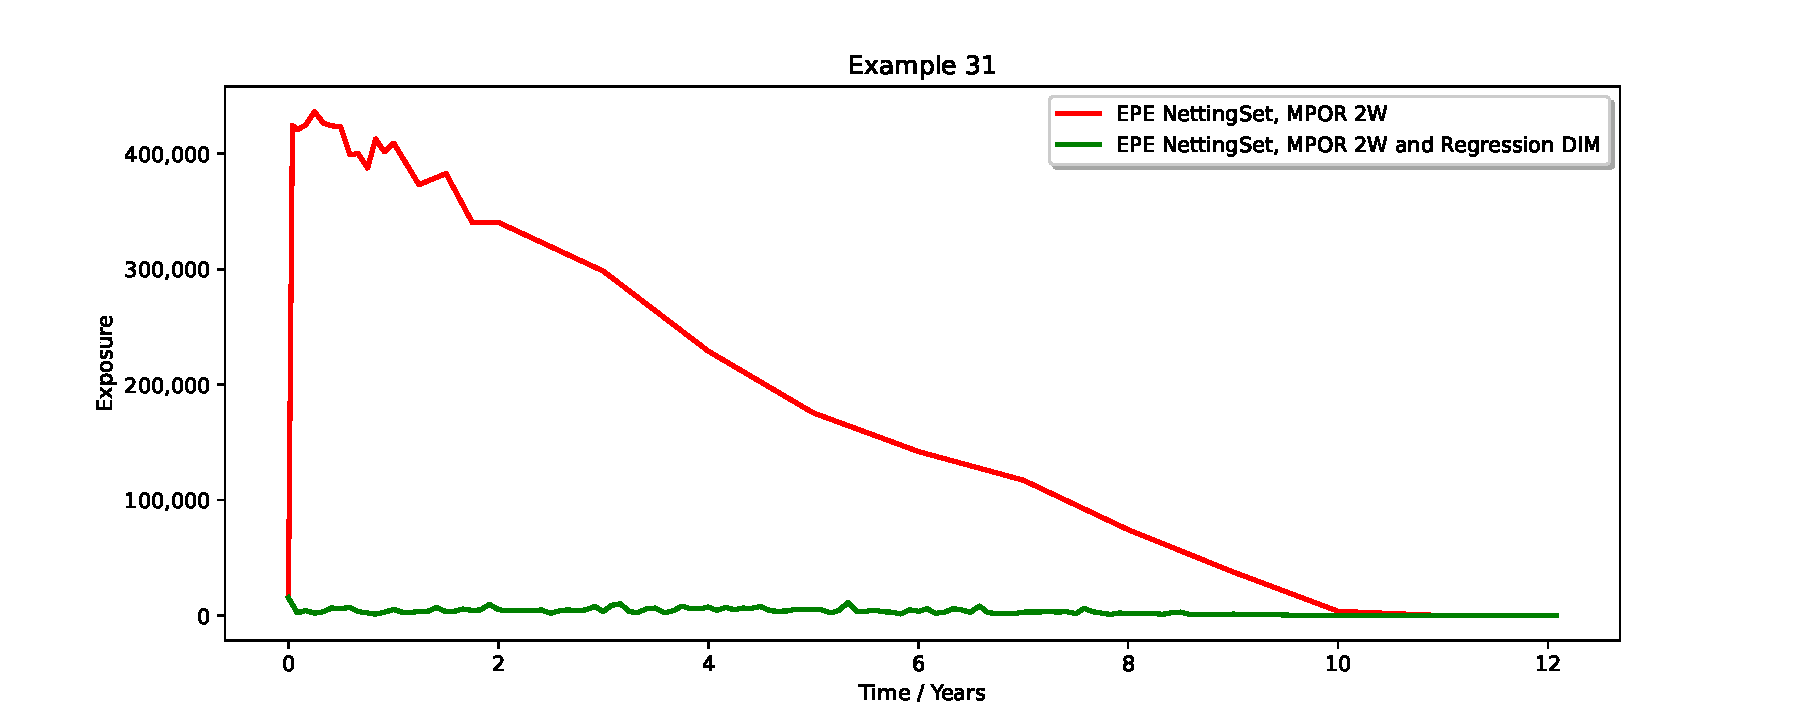
\includegraphics[scale=0.45]{examples/mpl_closeout_dim_epe.pdf}
\end{center}
\caption{Comparison of Swap exposure with VM only as above vs VM+IM using first-order regression.}
\label{fig_31_b}
\end{figure}

\begin{figure}[h!]
\begin{center}
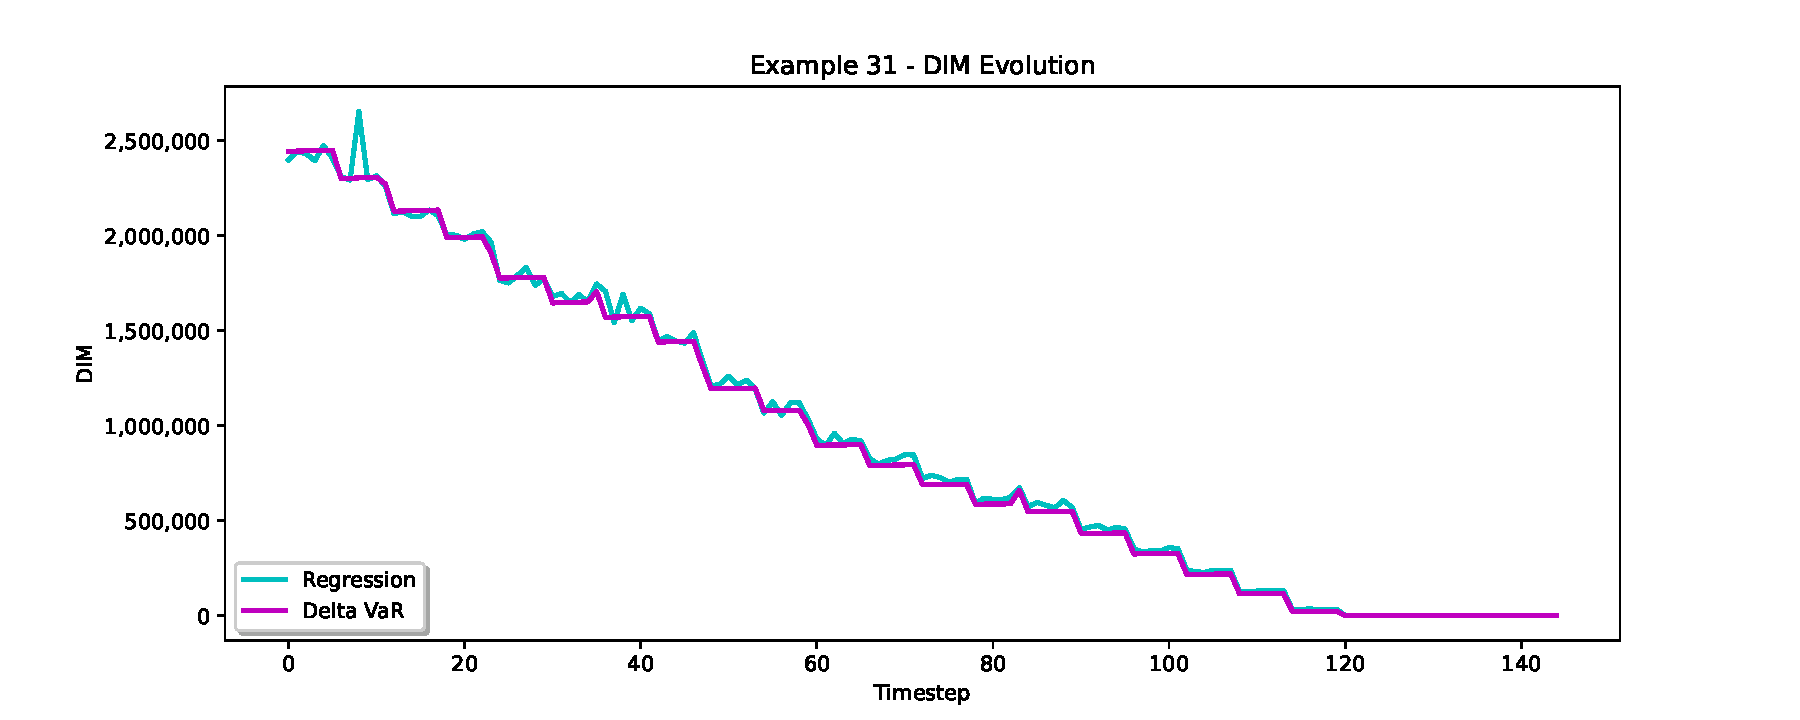
\includegraphics[scale=0.45]{examples/mpl_closeout_dim_evolution.pdf}
\end{center}
\caption{Evolution of expected IM from the regression model vs Delta VaR benchmark.}
\label{fig_31_c}
\end{figure}

The resulting exposure graphs, with comparison of the uncollateralised to the collateralised
case (with Variation Margin only) is shown in figure \ref{fig_31_a}.

In figure \ref{fig_31_b} we have added Initial Margin based on ORE's regression model, and we compare the exposure with VM only to
the exposure with both VM and IM. Figure \ref{fig_31_c} shows the related evolution of expected DIM, benchmarked against the
Delta VaR DIM model, used in section \ref{example:initialmargin_dim} and described in \cite{methods}.

\subsubsection{First MPoR Adjustment}

Calling

\medskip
\centerline{\tt python run\_firstmpor.py} 
\medskip

demonstrates a simple XVA calculation for a Receiver Swap (in netting set CPTY\_A) and a Payer Swap (in netting set CPTY\_B)
with two initial VM balances each such that the netting set is fully collateralised resp. over/under-collateralised.

The new flag firstMporCollateralAdjustment in ore.xml's XVA section affects the first MPoR, 2 weeks in the example.
If set to true, the difference between initial collateral balance and mtm is carried over during the first MPoRr period,
if the difference increases our exposure - a conservative measure.

\subsection{Scripted Trade}\label{example:scriptedtrade}

The scripted trade was added to ORE to gain more flexibility in representing exotic products, with hybrid payoffs across
asset classes, path-dependence, multiple kinds of early termination options. The scripted trade module uses Monte Carlo and
Finite Difference pricing approaches, it is an evolving interface to implement parallel processing with GPUs and a central
interface to implement AD methods in ORE. See the separate documentation in folder Docs/ScriptedTrade for an introduction to trade
representation, scripting language, model and pricing engine configuration. 

\medskip
The example in this folder {\tt Examples/ScriptedTrade} is a basic demonstration of ORE's scripted trade functionality.
In this example we provide a self-contained case that can be run as usual calling

\medskip
\centerline{\tt python run.py}

\medskip

This generates an NPV and cash flow report for the following portfolio
\begin{itemize}
\item Trade 1: Vanilla European Equity Option, represented as standard ORE XML with analytical pricing
\item Trade 2: Same Option as above, represented as ``generic'' scripted trade with scripted payoff embedded into the trade XML,
  pricing via Monte Carlo
\item Trade 3: Same Option as above, same representation, pricing via Finite Differences triggered by a {\tt ProductTag} assigned
  to the script and used in {\tt pricingengine.xml} 
\item Trade 4: Same Option as above, the scripted trade now refers to an ``external'' script in {\tt scriptlibrary.xml},
  MC pricing
\item Trade 4b: Same as trade 4, but ``compact'' scripted trade representation (uncomment trade 4b in {\tt portfolio.xml})
\item Trade 5: Barrier Option with single continuously observed Up \& Out barrier, represented as standard ORE XML with
  analytical pricing
\item Trade 6: Same Barrier Option as above, approximated as generic scripted trade with daily barrier observation
\item Trade 6b: Same Barrier Option as above, approximated as ``compact'' scripted trade with daily barrier observation
  (uncomment trade 6b in {\tt portfolio.xml})
\item Trade 7: Same Barrier Option as above, represented as generic scripted trade with continuously observed barrier,
  i.e. adjusting for the probability of knock-out between daily observations
\item Trade 7b: Same Barrier Option as of above, represented as ``compact'' scripted trade
  (uncomment trade 7b in {\tt portfolio.xml})
\item Trade 8: Equity Accumulator, represented as generic scripted trade with external payoff script
\item Trade 8b: Same Equity Accumulator as above, represented as compact scripted trade with external payoff script
  (uncomment trade 8b in {\tt portfolio.xml})
\end{itemize}

Note:
\begin{itemize}
\item In all cases we use the Black-Scholes model to drive the Equity process.
\item The Barrier Option pricing using the scripted trade deviates noticeably from the analytical pricing when we use daily
  observations (trade 6 and 6b), but matches quite closely when we adjust for the probability of knock-out between observation
  dates (trade 7 and 7b)
\item We are not aware of analytical pricing for the Accumulator product in trade 8 to benchmark against; trade 8 is priced with MC,
  FD pricing of the Accumulator is possible as well but requires a separate payoff script, only in the vanilla European option case
  we can utilize the same script for both MC and FD pricing
\end{itemize}

Though this initial example shows only single-asset Equity cases, the scripted trade in its current version is
significantly more versatile, more examples and scripts to follow.

\subsection{American Monte Carlo}\label{example:amc}

The cases in this section, folder {\tt AmericanMonteCarlo},  demonstrate how to use American Monte Carlo Simulation (AMC)
to generate exposures in ORE.
\begin{itemize}
\item We start with benchmarking against "classic" exposure simulation, i.e. 
  we run both AMC and classic simulation on a small IR/FX portfolio, almost vanilla, that
  consists of a Bermudan Swaption, Single and Cross Currency Swaps, FX Swap and FX Option,
  and we compare the resulting AMC vs. classic exposures. \\
  Run with {\tt python run\_benchmark.py}
\item Scripted Bermudan Swaption and LPI Swap: This case shows that the scripted trade
  framework works with AMC too, demonstrated here with a scripted Bermudan Swaption and an LPI Swap. \\
  Run with: {\tt python run\_scriptedberm.py}
\item FX TaRF: FxTaRF product is implemented using the scripted trade framework "under the hood"
  with the payoff script embedded into C++, so that it is neither explicit in the trade XML nor
  in the script library.\\
  Run with: {\tt python run\_fxtarf.py}
\item Forward Bond with AMC, run with: {\tt python run\_forwardbond.py}
\item Overlapping Close-Out Grid, run with: {\tt python run\_overlapping.py}
\item Scenario Statistics, run with: {\tt python run\_scenariostatistics.py}
\end{itemize}

\subsubsection{Benchmarking AMC vs Classic Simulation}

This example demonstrates how to use American Monte Carlo simulation (AMC) to generate exposures in ORE.
For a sketch of the methodology and comments on its implementation in ORE see \cite{methods}.
Moreover we discuss the essential configuration chnages for applying AMC.

Calling 

\medskip
\centerline {\tt python run\_benchmark.py} 

\medskip
performs two ORE runs, a 'classical' exposure simulation and an American Monte Carlo simulation, both on a
quarterly simulation grid and for the same portfolio consisting of four trades:

\begin{itemize}
\item Bermudan swaption
\item Single Currency Swap
\item Cross Currency Swap
\item FX Option
\end{itemize}

We use a 'flat' market here (yield curve and Swaption volatility surface). The number of simulation paths
is 2k in the classic simulations. If not stated otherwise below, the number of training paths and simulation
paths is 10k in the AMC simulations. 

In the following we compare the AMC exposure profiles to those produced by the 'classic' valuation engine
for each trade and the netting set. 

Figure \ref{epe_swaption} shows the EPE and ENE for a Bermudan Swaption 10y into 10y in (base ccy) EUR with
physical settlement. The classic run uses the LGM grid engine for valuation. We observe close agreement between
the two runs. To achieve the observed agreement, it is essential to set the LGM model's mean reversion speed
to zero in both
\begin{itemize}
\item the Bermudan Swaption LGM pricing model (see Input/pricingengine.xml), and
\item the Cross Asset Model's IR model components (see Input/simulation.xml and Input/simulation\_amc.xml) 
\end{itemize}
and to use a high order 6 of the regression polynomials (see Input/pricingengine\_amc.xml).
 
\begin{figure}
  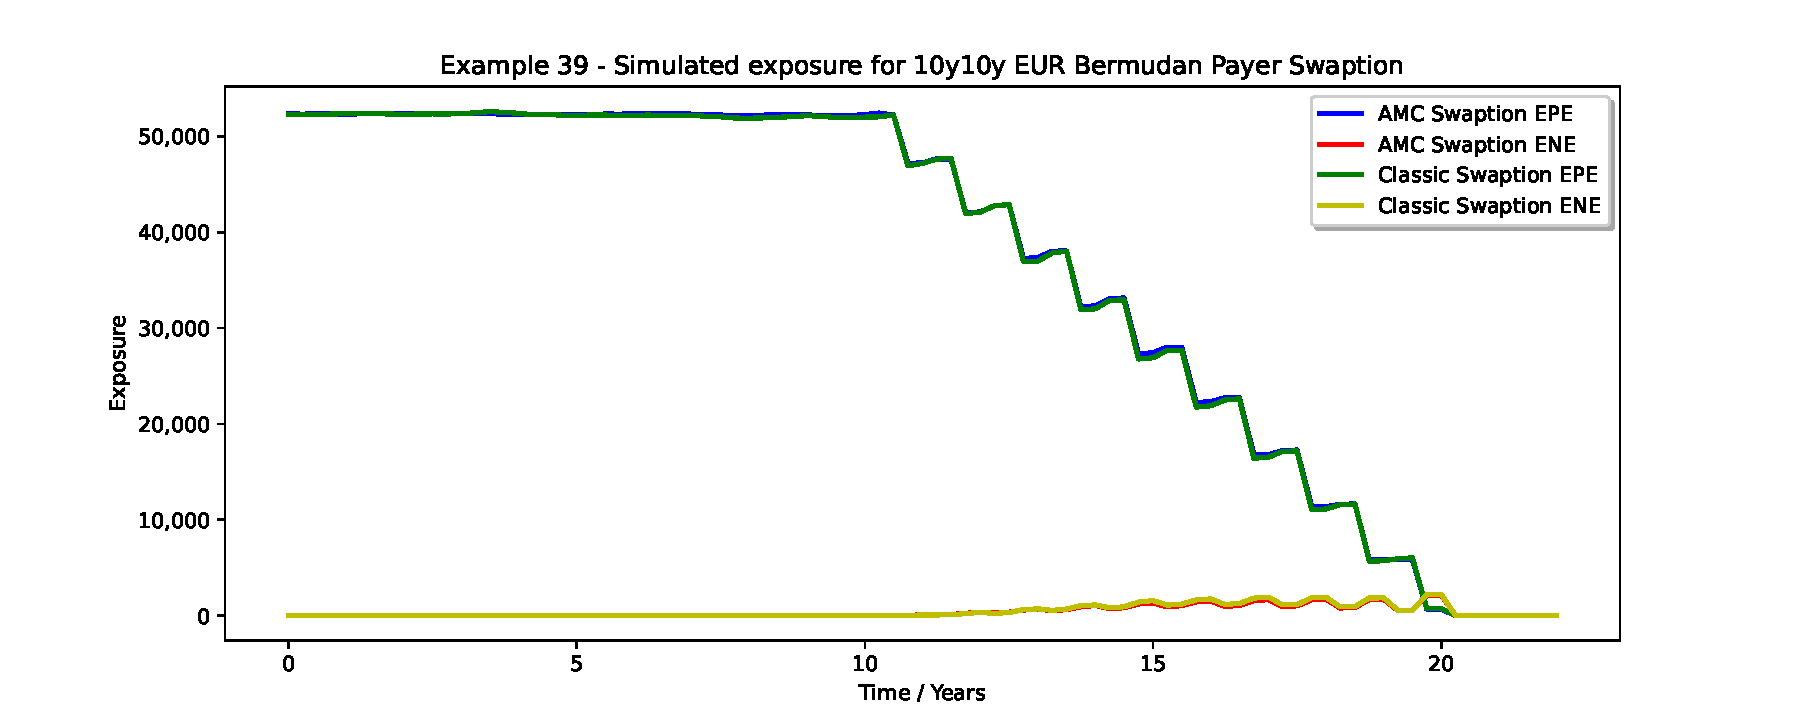
\includegraphics[width=0.8\textwidth]{examples/mpl_amc_bermudanswaption.pdf}
  \caption{EPE of a EUR Bermudan Swaption computed with the classic and AMC valuation engines, using 50k
    training paths for the AMC simulation.}
  \label{epe_swaption}
\end{figure}

Figure \ref{epe_swap} shows the EPE and ENE for a 20y vanilla Swap in USD. The currency of
the amc calculator is USD in this case, i.e. it is different from the base ccy of the simulation (EUR).
The consistency of the classic and amc runs in particular demonstrates the correct application of the currency
conversion factor (see methodology guide). To get a better accuracy for purposes of the plot in this document
we increased the number of training paths for this example to 50k and the order of the basis functions to 6.

\begin{figure}
  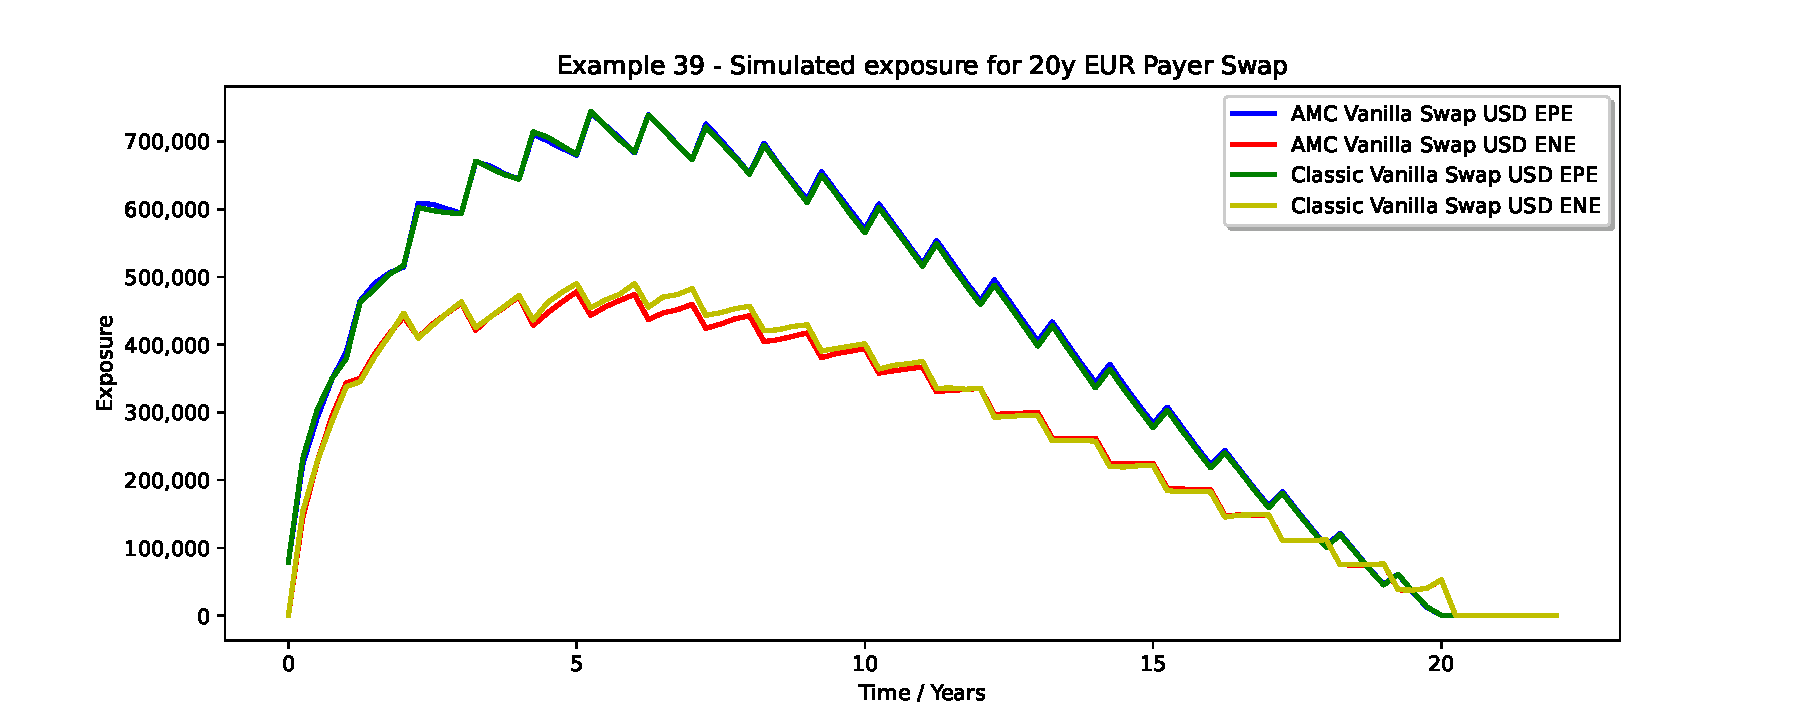
\includegraphics[width=0.8\textwidth]{examples/mpl_amc_vanillaswap_usd.pdf}
  \caption{EPE of a USD swap computed with the classic and AMC valuation engines}
  \label{epe_swap}
\end{figure}

Figure \ref{epe_ccyswap} shows the EPE and ENE for a 20y cross currency Swap EUR-USD. 

\begin{figure}
  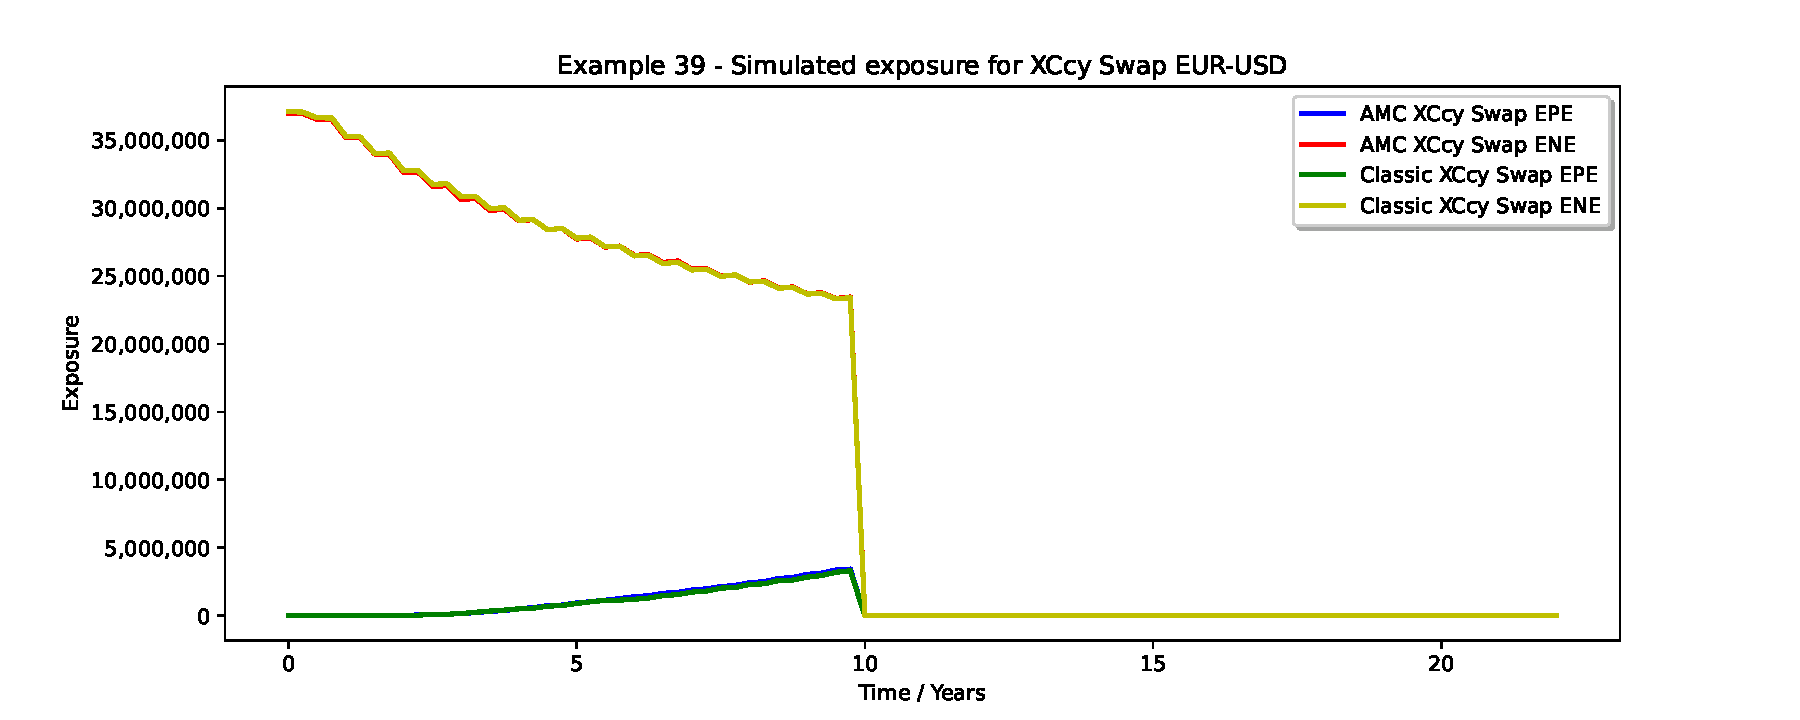
\includegraphics[width=0.8\textwidth]{examples/mpl_amc_xccyswap.pdf}
  \caption{EPE of a EUR-USD cross currency swap computed with the classic and AMC valuation engines}
  \label{epe_ccyswap}
\end{figure}

Figure \ref{epe_fxoption} shows the EPE and ENE for a vanilla FX Option EUR-USD with 10y1m expiry. 
For the classic run the FX volatility surface is not implied by the cross asset model but kept flat, which
yields a slight hump in the profile. The AMC profile is flat on the other hand which demonstrates the
consistency of the FX Option pricing with the risk factor evolution model.

\begin{figure}
  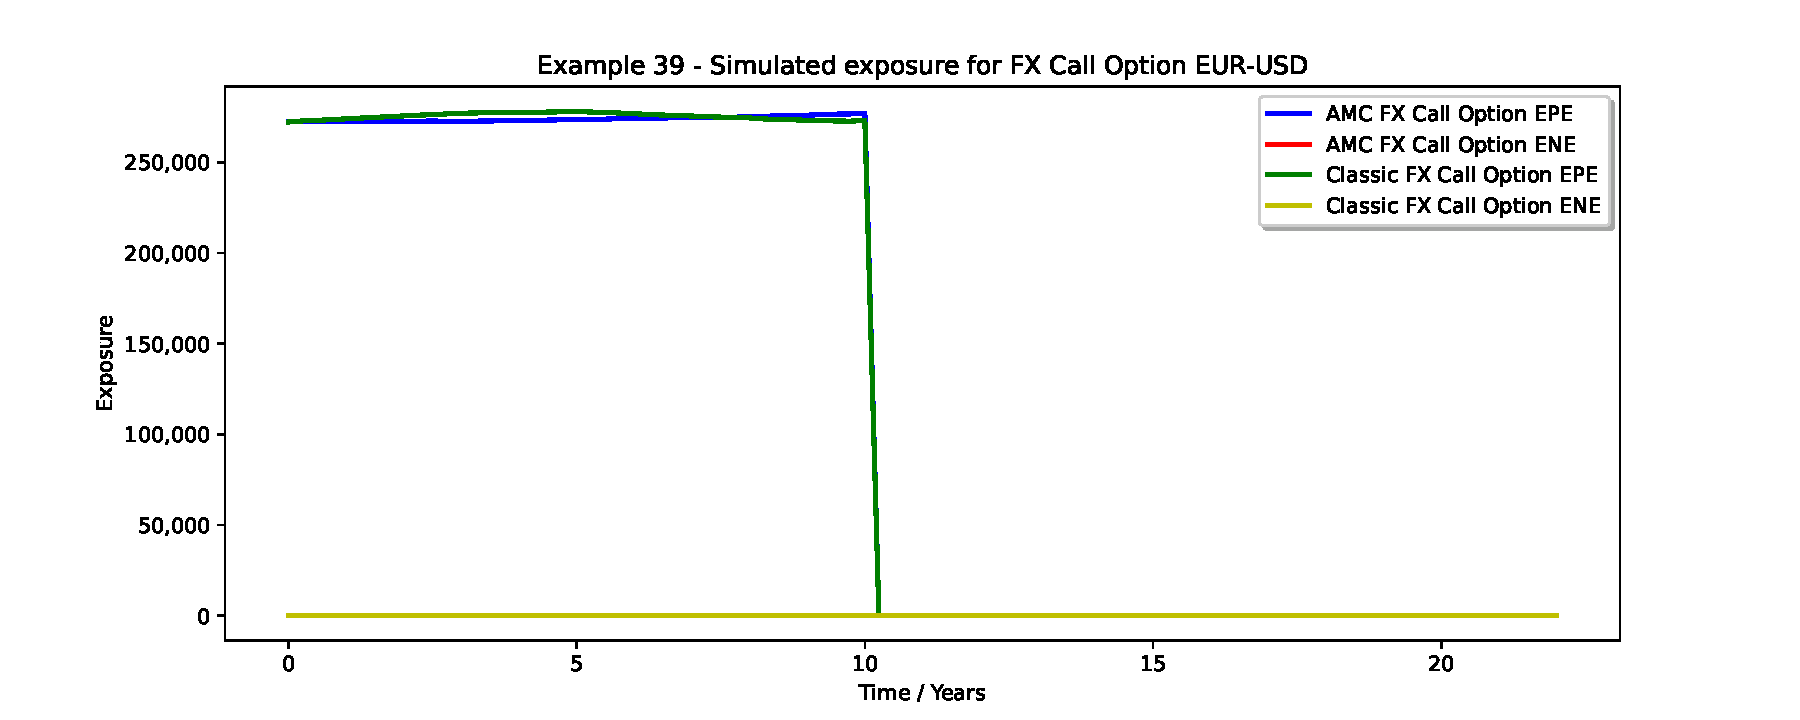
\includegraphics[width=0.8\textwidth]{examples/mpl_amc_fxoption.pdf}
  \caption{EPE of a EUR-USD FX option computed with the classic and AMC valuation engines}
  \label{epe_fxoption}
\end{figure}

\subsubsection*{Analytic Configuration}
\label{sec:amc_applicationconfig}

To use the AMC engine for an XVA simulation the following needs to be added to the {\tt simulation} analytic
in {\tt ore.xml}:

\begin{minted}[fontsize=\scriptsize]{xml}
<Analytic type="simulation">
  ...
  <Parameter name="amc">Y</Parameter>
  <Parameter name="amcPricingEnginesFile">pricingengine_amc.xml</Parameter>
  <Parameter name="amcTradeTypes">Swaption</Parameter>
  ...
</Analytic>
\end{minted}

The trades which have a trade type matching one of the types in the \verb+amcTradeTypes+ list, will be built against the
pricing engine config provided and processed in the AMC engine. As a naming convention, pricing engines with engine type
AMC provide the required functionality to be processed by the AMC engine, for technical details cf. \cite{methods}.

All other trades are processed by the classic simulation engine in ORE. The resulting cubes from the classic and AMC
simulation are joined and passed to the post processor in the usual way.

Note that since sometimes the AMC pricing engines have a different base ccy than the risk factor evolution model (see
below), a horizon shift parameter in the simulation set up should be set for all currencies, so that the shift also
applies to these reduced models.

\subsubsection*{Pricing Engine Configuration}
\label{sec:amc_pricingengineconfig}

At this point we assume that the reader is generally familiar with the configuration section 
\ref{sec:configuration}, in particular pricing engine configuration in section in \cite{products}.

The pricing engine configuration is similar for all AMC enabled products, e.g. for Bermudan Swaptions:

\begin{minted}[fontsize=\scriptsize]{xml}
<Product type="BermudanSwaption">
  <Model>LGM</Model>
  <ModelParameters/>
  <Engine>AMC</Engine>
  <EngineParameters>
    <Parameter name="Training.Sequence">MersenneTwisterAntithetic</Parameter>
    <Parameter name="Training.Seed">42</Parameter>
    <Parameter name="Training.Samples">50000</Parameter>
    <Parameter name="Training.BasisFunction">Monomial</Parameter>
    <Parameter name="Training.BasisFunctionOrder">6</Parameter>
    <Parameter name="Pricing.Sequence">SobolBrownianBridge</Parameter>
    <Parameter name="Pricing.Seed">17</Parameter>
    <Parameter name="Pricing.Samples">0</Parameter>
    <Parameter name="BrownianBridgeOrdering">Steps</Parameter>
    <Parameter name="SobolDirectionIntegers">JoeKuoD7</Parameter>
    <Parameter name="MinObsDate">true</Parameter>
    <Parameter name="RegressionOnExerciseOnly">false</Parameter>
  </EngineParameters>
</Product>
\end{minted}

The \verb+Model+ differs by product type, table \ref{tbl:amcconfig} summarises the supported product types and model and
engine types. The engine parameters are the same for all products:

\begin{enumerate}
\item \verb+Training.Sequence+: The sequence type for the training phase, can be \verb+MersenneTwister+,
  \verb+MersenneTwisterAntithetc+, \verb+Sobol+, \verb+Burley2020Sobol+, \verb+SobolBrownianBridge+,
  \verb+Burley2020SobolBrownianBridge+
\item \verb+Training.Seed+: The seed for the random number generation in the training phase
\item \verb+Training.Samples+: The number of samples to be used for the training phase
\item \verb+Pricing.Sequence+: The sequence type for the pricing phase, same values allowed as for training
\item \verb+Training.BasisFunction+: The type of basis function system to be used for the regression analysis, can be
  \verb+Monomial+, \verb+Laguerre+, \verb+Hermite+, \verb+Hyperbolic+, \verb+Legendre+, \verb+Chbyshev+,
  \verb+Chebyshev2nd+
\item \verb+BasisFunctionOrder+: The order of the basis function system to be used
\item \verb+Pricing.Seed+: The seed for the random number generation in the pricing
\item \verb+Pricing.Samples+: The number of samples to be used for the pricing phase. If this number is zero, no pricing
  run is performed, instead the (T0) NPV is estimated from the training phase (this result is used to fill the T0 slice
  of the NPV cube)
\item \verb+BrownianBridgeOrdering+: variate ordering for Brownian bridges, can be \verb+Steps+, \verb+Factors+,
  \verb+Diagonal+
\item \verb+SobolDirectionIntegers+: direction integers for Sobol generator, can be \verb+Unit+, \verb+Jaeckel+,
  \verb+SobolLevitan+, \verb+SobolLevitanLemieux+, \verb+JoeKuoD5+, \verb+JoeKuoD6+, \verb+JoeKuoD7+,
  \verb+Kuo+, \verb+Kuo2+, \verb+Kuo3+
\item \verb+MinObsDate+: if true the conditional expectation of each cashflow is taken from the minimum possible
  observation date (i.e. the latest exercise or simulation date before the cashflow's event date); recommended setting
  is \verb+true+
\item \verb+RegressionOnExerciseOnly+: if true, regression coefficients are computed only on exercise dates and
  extrapolated (flat) to earlier exercise dates; only for backwards compatibility to older versions of the AMC module,
  recommended setting is \verb+false+
\end{enumerate}

\begin{table}[hbt]
  \begin{tabular}{l|l|l}
    Product Type & Model & Engine \\ \hline
    Swap & CrossAssetModel & AMC \\
    CrossCurrencySwap & CrossAssetModel & AMC \\
    FxOption & CrossAssetModel & AMC \\
    BermudanSwaption & LGM & AMC \\
    MultiLegOption & CrossAssetModel & AMC \\
  \end{tabular}
  \caption{AMC enabled products with engine and model types}
  \label{tbl:amcconfig}
\end{table}

\subsubsection*{Additional Features}
\label{sec:amc_sideproducts}

As a side product the AMC module provides plain MC pricing engines for Bermudan Swaptions and a new trade type
\verb+MultiLegOption+ with a corresponding MC pricing engine.

\subsubsection*{MC pricing engine for Bermudan swaptions}\label{sec:mc_bermudan_engine}

The following listing shows a sample configuration for the MC Bermudan Swaption engine. The model parameters are
identical to the LGM Grid engine configuration. The engine parameters on the other hand are the same as for the AMC
engine, see \ref{sec:amc_pricingengineconfig}.

\begin{minted}[fontsize=\scriptsize]{xml}
<Product type="BermudanSwaption">
  <Model>LGM</Model>
  <ModelParameters>
    <Parameter name="Calibration">Bootstrap</Parameter>
    <Parameter name="CalibrationStrategy">CoterminalDealStrike</Parameter>
    <Parameter name="Reversion_EUR">0.0050</Parameter>
    <Parameter name="Reversion_USD">0.0030</Parameter>
    <Parameter name="ReversionType">HullWhite</Parameter>
    <Parameter name="VolatilityType">HullWhite</Parameter>
    <Parameter name="Volatility">0.01</Parameter>
    <Parameter name="ShiftHorizon">0.5</Parameter>
    <Parameter name="Tolerance">1.0</Parameter>
  </ModelParameters>
  <Engine>MC</Engine>
  <EngineParameters>
    <Parameter name="Training.Sequence">MersenneTwisterAntithetic</Parameter>
    <Parameter name="Training.Seed">42</Parameter>
    <Parameter name="Training.Samples">10000</Parameter>
    <Parameter name="Training.BasisFunction">Monomial</Parameter>
    <Parameter name="Training.BasisFunctionOrder">6</Parameter>
    <Parameter name="Pricing.Sequence">SobolBrownianBridge</Parameter>
    <Parameter name="Pricing.Seed">17</Parameter>
    <Parameter name="Pricing.Samples">25000</Parameter>
    <Parameter name="BrownianBridgeOrdering">Steps</Parameter>
    <Parameter name="SobolDirectionIntegers">JoeKuoD7</Parameter>
  </EngineParameters>
</Product>
\end{minted}

\subsubsection*{Multi Leg Options / MC pricing engine}

The following listing shows a sample MultiLegOption trade. It consists of

\begin{enumerate}
\item an option data block; this is optional, see below
\item a number of legs; in principle all leg types are supported, the number of legs is arbitrary and they can be in
  different currencies; if the payment currency of a leg is different from a floating index currency, this is
  interpreted as a quanto payoff
\end{enumerate}

If the option block is given, the trade represents a Bermudan swaption on the underlying legs. If the option block is
missing, the legs themselves represent the trade.

See \cite{methods} for limitations of the multileg option pricing engine.

\begin{minted}[fontsize=\scriptsize]{xml}
<Trade id="Sample_MultiLegOption">
  <TradeType>MultiLegOption</TradeType>
  <Envelope>...</Envelope>
  <MultiLegOptionData>
    <OptionData>
      <LongShort>Long</LongShort>
      <OptionType>Call</OptionType>
      <Style>Bermudan</Style>
      <Settlement>Physical</Settlement>
      <PayOffAtExpiry>false</PayOffAtExpiry>
      <ExerciseDates>
        <ExerciseDate>2026-02-25</ExerciseDate>
        <ExerciseDate>2027-02-25</ExerciseDate>
        <ExerciseDate>2028-02-25</ExerciseDate>
      </ExerciseDates>
    </OptionData>
    <LegData>
      <LegType>Floating</LegType>
      <Payer>false</Payer>
      <Currency>USD</Currency>
      <Notionals>
        <Notional>100000000</Notional>
      </Notionals>
      ...
    </LegData>
    <LegData>
      <LegType>Floating</LegType>
      <Payer>true</Payer>
      <Currency>EUR</Currency>
      <Notionals>
        <Notional>100000000</Notional>
      </Notionals>
      ...
    </LegData>
  </MultiLegOptionData>
</Trade>
\end{minted}

The pricing engine configuration is similar to that of the MC Bermudan swaption engine, cf.
\ref{sec:mc_bermudan_engine}, also see the following listing.

\begin{minted}[fontsize=\scriptsize]{xml}
  <Product type="MultiLegOption">
  <Model>CrossAssetModel</Model>
  <ModelParameters>
    <Parameter name="Tolerance">0.0001</Parameter>
    <!-- IR -->
    <Parameter name="IrCalibration">Bootstrap</Parameter>
    <Parameter name="IrCalibrationStrategy">CoterminalATM</Parameter>
    <Parameter name="ShiftHorizon">1.0</Parameter>
    <Parameter name="IrReversion_EUR">0.0050</Parameter>
    <Parameter name="IrReversion_GBP">0.0070</Parameter>
    <Parameter name="IrReversion_USD">0.0080</Parameter>
    <Parameter name="IrReversion">0.0030</Parameter>
    <Parameter name="IrReversionType">HullWhite</Parameter>
    <Parameter name="IrVolatilityType">HullWhite</Parameter>
    <Parameter name="IrVolatility">0.0050</Parameter>
    <!-- FX -->
    <Parameter name="FxCalibration">Bootstrap</Parameter>
    <Parameter name="FxVolatility_EURUSD">0.10</Parameter>
    <Parameter name="FxVolatility">0.08</Parameter>
    <Parameter name="ExtrapolateFxVolatility_EURUSD">false</Parameter>
    <Parameter name="ExtrapolateFxVolatility">true</Parameter>
    <!-- Correlations IR-IR, IR-FX, FX-FX -->
    <Parameter name="Corr_IR:EUR_IR:GBP">0.80</Parameter>
    <Parameter name="Corr_IR:EUR_FX:GBPEUR">-0.50</Parameter>
    <Parameter name="Corr_IR:GBP_FX:GBPEUR">-0.15</Parameter>
  </ModelParameters>
  <Engine>MC</Engine>
  <EngineParameters>
    <Parameter name="Training.Sequence">MersenneTwisterAntithetic</Parameter>
    <Parameter name="Training.Seed">42</Parameter>
    <Parameter name="Training.Samples">10000</Parameter>
    <Parameter name="Pricing.Sequence">SobolBrownianBridge</Parameter>
    <Parameter name="Pricing.Seed">17</Parameter>
    <Parameter name="Pricing.Samples">25000</Parameter>
    <Parameter name="Training.BasisFunction">Monomial</Parameter>
    <Parameter name="Training.BasisFunctionOrder">4</Parameter>
    <Parameter name="BrownianBridgeOrdering">Steps</Parameter>
    <Parameter name="SobolDirectionIntegers">JoeKuoD7</Parameter>
  </EngineParameters>
</Product>
\end{minted}

Model Parameters special to that product are

\begin{enumerate}
\item \verb+IrCalibrationStrategy+ can be \verb+None+, \verb+CoterminalATM+, \verb+UnderlyingATM+
\item \verb+FXCalibration+ can be \verb+None+ or \verb+Bootstrap+
\item \verb+ExtrapolateFxVolatility+ can be \verb+true+ or \verb+false+; if false, no calibration instruments are used
  that require extrapolation of the market fx volatility surface in option expiry direction
\item \verb+Corr_Key1_Key2+: These entries describe the cross asset model correlations to be used; the syntax for
  \verb+Key1+ and \verb+Key2+ is the same as in the simulation configuration for the cross asset model
\end{enumerate}


\subsubsection{Scripted Bermudan}

Calling 

\medskip
\centerline {\tt python run\_scriptedberm.py} 

\medskip
demonstrates exposure simulation using AMC for selected scripted trade types
\begin{itemize}
\item Bermudan Swaption
\item LPI Swap
\end{itemize}
Both payoffs are defined in the {\tt scriptlibrary.xml} which are referenced in {\tt portfolio\_scriptedberm.xml}
by the {\tt ScriptName} tag. \\

To enable the AMC processing requires the following highlighted settings in {\tt ore.xml}.

\begin{minted}[fontsize=\scriptsize]{xml}
    <Analytic type="simulation">
      <Parameter name="active">Y</Parameter>
      <!-- Set to Y to trigger AMC processing -->
      <Parameter name="amc">Y</Parameter>
      <Parameter name="simulationConfigFile">simulation.xml</Parameter>
      <Parameter name="pricingEnginesFile">pricingengine.xml</Parameter>
      <!-- Specify a separate pricing engine file for AMC engines -->
      <Parameter name="amcPricingEnginesFile">pricingengine\_amc.xml</Parameter>
      <!-- Specify trade types to be covered by the AMC processing -->
      <Parameter name="amcTradeTypes">ScriptedTrade</Parameter>
      <Parameter name="baseCurrency">EUR</Parameter>
      <Parameter name="cubeFile">cube.csv.gz</Parameter>
      <Parameter name="aggregationScenarioDataFileName">scenariodata.csv.gz</Parameter>
      <Parameter name="aggregationScenarioDataDump">scenariodata.csv</Parameter>
    </Analytic>
\end{minted}

Note that ORE can handle a mix of trades covered by AMC simulation and covered by ``classic'' simulation.
The respective NPV cubes are combined before generating results such as exposures or XVAs.

\subsubsection{Scripted TaRF}

Calling 

\medskip
\centerline {\tt python run\_scriptedtarf.py} 

\medskip
demonstrates exposure simulation and XVA for another scripted product, an
FX Target Redemption Forward (TaRF). In contrast to the cases presented above, you won't see
the payoff script library in the Input folder, nor is the script embedded into the trade XML file.
The trade type in this case is {\tt FxTARF} which has its own implementation in {\tt OREData/ored/portfolio/tarf.xpp}
and a separate trade schema. However, the scripted trade framework is used under the hood, and the payoff
script is embedded into the C++ code in OREData/ored/portfolio/tarf.cpp.

\subsubsection{Forward Bond}

Calling 

\medskip
\centerline {\tt python run\_forwardbond.py} 

\medskip
demonstrates AMC exposure simulation and XVA for a forward and a plain vanilla bond.
The results can be compared to a classical exposure simulation by switchting the parameter \emph{amc} in the
main configuration file \emph{ore.xml}, section analytic type \emph{Simulation} to \emph{N}.

For both cases, forward and plain vanilla bond, the security spread is implied from given bond prices.
This requires a proper security specification in the curve configuration. Compare \emph{Securities} node
within \emph{curveconfig.xml}. Both fields, PriceQuote and SpreadQuote, are mandatory. In the market data file,
if the price quote is given in the absence of a spread quote, the spread is implied.
Otherwise the spread quote is used or none.

In case of a forward bond, the convention for security specification requires the format \emph{securityId\_FWDEXP\_expiryDate}.

\subsubsection{Overlapping Close-out Grids in AMC}

Calling 

\medskip
\centerline {\tt python run\_overlapping.py} 

\medskip
demonstrates the case where the primary and close-out grid overlap, using
a daily simulation grid up to 15 days. This was not possible in releases earlier than ORE v13.

\subsubsection{Extract Scenario Statistics}

Calling 

\medskip
\centerline {\tt python run\_scenariostatistics.py} 

\medskip
demonstrates a basic statistical anylsis of the simulated raw scenario data (simulated yield curve discount factors, FX spot rates etc), generating a report
with min, mean, max, standard deviation, skewness and kurtosis for each factor and at each simulated future date.

\subsection{XVA Risk}\label{example:xvarisk}

The following XVA Risk-related examples can be found in folder {\tt Examples/XvaRisk}.
They can be run individually as discussed below, or all together with: {\tt python run.py} 

\subsubsection{XVA Stress Testing}\label{example:xvarisk_stress}

Calling

\medskip
\centerline {\tt python run\_stress.py} 

\medskip
demonstrates the XVA stress testing analytic using both classical and AMC XVA engine,
with output in {\tt Examples/XvaRisk/Output/stress}.

The new analytic type \emph{XVA\_STRESS} utilizes the existing stresstest framework and supports
stress tests in both zero and par domain. 
The stress test scenarios are given in the same input format as for the regular stresstest. 

To analyse the impact of market rate shifts (Swap rates, CDS spreads, flat vols), one had to
manipulate the market data input into ORE and re-run the entire ORE process multiple times.

The generated outputs are the xva and exposure reports under each scenario.

The XVA stress analytic replaces the todays market with a simulation market during the XVA calculation.
For some risk factors the simulation market behaves different from todays market.
Depending on the simulation and stress scenario settings it could use different tenors when building curves 
or use only ATM volatilities. It is recommended to activate {\tt UseSpreadedTermStructures} in the
{\tt stresstest.xml} and to simulate SwaptionVolatilities for the XVA stress run.

\subsubsection{XVA P\&L Explain}\label{example:xvarisk_pnl}

Calling

\medskip
\centerline {\tt python run\_xvaexplain.py} 

\medskip
demonstrates the XVA Explain Analytic with results in {\tt XvaRisk/Output/explain}.

ORE can compute the market implied XVA change between two evaluation dates.
For each risk factor defined in the sensitivity config ORE computes the par rate change between t0
and t0 + mporDays.  ORE derives for each risk factor a shift scenario ($ParRate(t_1) - ParRate(t_0)$)
and computes the CVA change implied by those risk factor shifts at t0.

Like the XVA Stress analytic,
the XVA Explain analytic replaces the todays market with a simulation market during the XVA calculation.
For some risk factors the simulation market behaves different from todays market.
Depending on the simulation and stress scenario settings it could use different tenors when building curves 
or use only ATM volatilities. It is recommended to activate {\tt UseSpreadedTermStructures} in
{\tt sensitivity\_explain.xml} and to simulate SwaptionVolatilities for the XVA Explain run
in {\tt xvaexplainmarket.xml}

\subsubsection{XVA Sensitivities}\label{example:xvarisk_sensi}

Calling

\medskip
\centerline {\tt python run\_sensi.py} 

\medskip
demonstrates the XVA Sensitivity analytic with results in {\tt XvaRisk/Output/sensi}, in particular
{\tt sacva.csv} and {\tt sacvadetail.csv}.

The analytic computes XVA sensitivities by bump \& revalue and generates the sensitivity scenarios from a
sensitivity configuration similar to the one used in NPV sensitivity calculation. It utilises the existing
XVA machinery ``under the hood'', supports XVA calculation using ``classic'' and AMC simulation.
Sensitivities are generated in both the ``raw'' (e.g. zero rate) domain as well as in the par domain.

This analysis is run twice here, with ``classic'' and AMC simulation, for a small proof-of-concept
``portfolio'' consisting of two swaps. We are running an (unusual) uncollateralised case here. The user
can activate both VM and IM as shown in previous examples.

For methodology summaries and the current scope of the implementations see \cite{methods}.

Note:
\begin{itemize}
\item The XVA sensitivity analytic replaces the TodaysMarket with a SimulationMarket during
  the XVA calculation. This is a template for extending other ORE analytics (such as VaR) for exposing
  their evaluation under stressed markets.
\item Realistic portfolios may require large numbers of sensitivity scenarios and hence XVA simulations
  which makes SA-CVA computationally challenging in practice. AMC simulation for XVA instead of ``classic''
  simulation helps performance here. As a further performance enhancement we are working on a computation
  graph framework for XVA which supports GPU parallelization and AAD for XVA sensitivity, see example
  section \ref{example:performance}.
\end{itemize}

\subsubsection{CVA Capital: SA-CVA and BA-CVA}\label{example:xvarisk_capital}

Calling

\medskip
\centerline {\tt python run\_sacva.py} 

\medskip
demonstrates CVA Capital calculation using the Standard Approach ({\bf SA-CVA}) with results in
{\tt XvaRisk/Output/sacva}. This analytic utilises the former XVA sensitivity analytic, in particular
its CVA par sensitivity output. Alternatively, CVA sensitivity can passed as an input. The
demonstration here picks up the sensitivities computed before by the XVA Sesnitivity analytic and
written to {\tt Output/sensi/amc/xva\_par\_sensitivity\_cva.csv}, see {\tt Input/ore\_sacva.xml}.

\medskip
Similarly, calling
\medskip
\centerline {\tt python run\_bacva.py} 

\medskip
demonstrates CVA Capital calculation using the Basic Approach ({\bf BA-CVA}) with results in
{\tt XvaRisk/Output/bacva}. BA-CVA is based on the SA-CCR Exposure At Default implementation,
hence calls the SA-CCR analytic ``under the hood''. SA-CCR is covered in section
\ref{example:creditrisk}. 

\subsection{Credit Risk}\label{example:creditrisk}

\subsubsection{SA-CCR}\label{example:creditrisk_saccr}

Calling
\medskip
\centerline {\tt python run\_saccr.py} 

\medskip
demonstrates the ``Standard Approach Counterparty Credit Risk (SA-CCR)'' Capital calculation for
derivatives in ORE with results in {\tt CreditRisk/Output/SA-CCR}, in particular {\tt saccr.csv}
and {\tt saccr\_detail.csv}. See \cite{methods} for the current implementaion's scope. 

\subsubsection{Credit Portfolio Model}\label{example:creditrisk_cpm}

The purpose of the credit portfolio model in ORE is to generate an integrated portfolio gain/loss distribution
at a given future horizon which is driven by 
\begin{itemize}
\item credit defaults and rating migrations in Bonds and CDS, and 
\item the PnL of a portfolio of derivatives over the specified time horizon.
\end{itemize}
The model integrates Credit and Market Risk by jointly evolving systemic credit risk drivers
alongside the usual risk factors in ORE's Cross Asset Model.
See also the separate documentation in {\tt Docs/UserGuide/creditmodel.tex|pdf}.
As mentioned there, this example will only run if the Eigen installation has been done before building ORE as described in section \ref{sec:build}.

By running \\
\medskip
\centerline{{\tt python run\_cpm.py}} 

\medskip
this example demonstrates the model's outcome for seven demo portfolios

\begin{center}
\begin{tabular}{|l|l|l|l|}
\hline
Case & Credit Mode & Exposure Mode & Evaluation \\
\hline
\hline
Single Bond & Migration & Value & Analytic \\
\hline
Bond and Swap & Migration & Value & Analytic \\
\hline
3 Bonds & Migration & Value & Analytic \\
\hline
10 Bonds & Migration & Value & Analytic \\
\hline
10 Bonds & Migration & Value & Terminal Simulation \\
\hline
Bonds and CDS & Migration & Notional & Analytic \\
\hline
100 Bonds & Default & Notional & Analytic \\
\hline
\end{tabular}
\end{center}
The last demo case in this table can be activated by uncommenting the corresponding section at the end of the {\tt run\_cpm.py}
script.

\subsection{Performance}\label{example:performance}

\subsubsection{Multi-threading}

Calling
\medskip
\centerline {\tt python run\_multithreading.py} 

\medskip
demonstrates the parallelisation of exposure simulation for a portfolio of eight Vanilla Swap copies, results in folder
{\tt Performance/Output/multi}. The multi-threaded valuation engine in ORE splits the portfolio into $n$ parts where
$n$ is the number of threads {\tt nThreads} specified in {\tt ore\_multi.xml}.

\subsubsection{NPV Sensitivities with AAD and GPUs}

Calling
\medskip
\centerline {\tt python run\_sensi.py} 

\medskip
demonstrates alternative ways of speeding up sensitivity calculations - using AAD or an external compute device.
The test portfolio consists of 
\begin{itemize}
\item Vanilla Equity Option
\item Equity Barrier Option
\item Equity Accumulator
\item Asian Basket Option
\item FX TaRFs
\end{itemize}
The sensitivity analysis is then run in four ways, see {\tt run\_sensi.py},
\begin{itemize}
\item with ``classic'' bump and revalue ((19 sec on Apple M2 Max))
\item as above but using the Computation Graph, see {\tt UseCG=true} in {\tt pricingengine\_cg.xml}, which
  is the basis for the following two approaches ((14 sec on Apple M2 Max))
\item using AAD, see {\tt pricingengine\_ad.xml} ((2.2 sec on Apple M2 Max))
\item using the external device if available, see {\tt pricingengine\_gpu.xml} (2.3 sec on Apple M2 Max with "OpenCL/Apple/Apple M2 Max" device) 
\end{itemize}
to compare sensitivities and performance. In the latter case we have set the external device in
{\tt pricingengine\_gpu.xml} to ``BasicCpu/Default/Default'' which mimics an external device on the CPU.
On a macbook pro (2023) with M2 Max processor, we can also choose  
``OpenCL/Apple/Apple M2 Max'' here (a 38 core GPU).
The Jupyter notebook {\tt ore\_aadsensi.ipynb} in this {\tt Examples/Performance} folder also kicks
off these four runs, but adds further commentary and visualises results.
To run this notebook you need to build the Python bindings for release 12 (or later)
or ``pip install'' ORE as discussed in section \ref{example:orepython}.

\subsubsection{CVA Sensitivities with AAD}

Calling
\medskip
\centerline {\tt python run\_cvasensi.py} 

\medskip
demonstrates a prototype CVA sensitivity calculation applying AAD to a single Swap instrument
with results in folder {\tt Performance/Output/cvasensi}.

This script executes four batches
\begin{itemize}
\item a ``base'' CVA calculation using AMC for reference (about 9 sec on Apple M2 Max)
\item a bump \& revalue CVA sensitivity calculation (about 48 sec on Apple M2 Max)
\item CVA sensitivity using AAD (about 2 sec on Apple M2 Max) 
\item CVA sensitivities with GPU parallelisation, porting the conditional expectation calculations
  to the external device is work in progress, hence no noticeable speedup to be reported yet
\end{itemize}

Run the corresponding Juypter notebook with: {\tt python -m jupyterlab ore\_cvasensi.ipynb \&} 

\subsection{ORE-Python}\label{example:orepython}

Since release 9 (March 2023) we provide easy access to ORE via a pre-compiled Python module. Some example scripts using
this ORE module are provided in this example, so change to this directory first

\medskip
{\tt cd Examples/ORE-Python} 

\medskip
The examples require Python 3. The ORE Python module is then installed with a one-liner, see step 3 below. However, to
separate ORE from any other Python environments on your machine, we recommend creating a virtual environment first.
In that case the steps are as follows. 

\begin{enumerate}
\item To create a virtual environment: {\tt python -m venv env1} 
\item To activate this environment on Windows: {\tt .{\bs}env1{\bs}Scripts{\bs}activate.bat}  \\
or on macOS/Linux: {\tt source env1/bin/activate }  
\item Then install the latest release of ORE:\\
{\tt pip install open-source-risk-engine } 
\item Try examples:\\
  \begin{itemize} 
  \item {\tt python ore.py} \\
    This demonstrates the Python-wrapped version of the ORE application that is also used in the command line application
    {\tt ore.exe}. We use it here to re-run the Swap exposure of {\tt Example\_1}. 
  \item {\tt python ore2.py} \\
    This extends the previous example and shows how to access and post-process ORE in-memory results in the Python
    framework without reading files. 
  \item {\tt python commodityforward.py} \\
    The ORE Python module also allows lower-level access to the QuantLib and QuantExt libraries, demonstrated here for
    a CommodityForward instrument defined in QuantExt. 
    Note that the ORE Python module contains the entire QuantLib Python functionality.
  \end{itemize}
  More use cases of the ORE Python module including Jupyter notebooks can be found in the ORE SWIG repository,
  in particular in folder OREAnalytics-SWIG/Python/Examples. 
\item You can deactivate the environment with {\tt deactivate} \\
  or even fully remove the environment again by removing the {\tt env1} folder.
\end{enumerate}

Finally, you can build the Python module and installable packages yourself following the instructions in sections
\ref{sec:oreswig} based on your local ORE code. 

\subsubsection*{Jupyter Notebook Examples}

With ORE release 13 we have merged the ORE-SWIG source code into the ORE repository and moved a range of related
Jupyter notebook examples into this ORE-Python folder, see folders Notebooks/Example\_1 to Notebooks/Example\_9.

To try, change e.g. to Notebooks/Example\_1 and launch the notebook there by calling

\medskip
{\tt python3 -m jupyterlab ore.ipynb \& }

\medskip
If not installed yet, this might require a

\medskip
{\tt python3 -m pip install jupyterlab }

\medskip
and some of the Jupyter notebooks require additional packages to be installed with pip:
\begin{itemize}
\item matplotlib
\item pandas
\item numpy
\item scipy
\item ipywidgets
\end{itemize}

\subsection{ORE-API}\label{example:oreapi}

Since release 12, ORE comes with a proof-of-concept implementation of a web service around ORE
that is written in Python, see folder {\tt Examples/ORE-API}.

The service is based on
\begin{itemize}
\item the flask web framework \url{https://flask.palletsprojects.com}, and
\item the ORE Python module which can be installed using \\
  {\tt pip install open-source-risk-engine} \\
  or built from sources following the instructions in section \ref{sec:installation}
\end{itemize}

\medskip
Main files in the {\tt Examples/API} directory:
\begin{itemize}
\item {\bf restapi.py} runs a flask api as analytics service that takes a post request
  (e.g. from a server like postman, or from a python script): The request contains a json body
  which corresponds to the data usually contained in the master input file ore.xml. restapi.py
  calls the oreApi.py class (see below) to do the work. By default, the analytics service listens for
  requests on port 5001.
\item {\bf oreApi.py} reads the json body, compiles all ORE input parameters, calls into a
  data service (see below) to retrieve additional data. Then it kicks off an ORE run to process
  the request.  Finally it posts resulting reports through the data service.
\item {\bf simplefileserver.py} runs a flask api as a data service. It takes requests from the
  analytics service above in the form of urls of xml files that contain additional data required
  by ORE (market data, portfolio, configuration). By default, the data service
  listens on port 5000, reads from the Input directory in Examples/API and writes reports to the Output
  directory in Examples/API.
\end{itemize}

\medskip
Run a local example:
\begin{itemize}
\item start the data service: \\
  {\tt python3 simplefileserver.py \&} 
\item start the analytics service: \\
  {\tt python3 restapi.py \&}
\item send a request to run the equivalent of Example 1: \\
  {\tt python3 request.py} \\
  Note that the json equivalent of the usual {\tt ore.xml} is contained in request.py,
  and all other inputs are retrieved from folder Examples/API/Input via the data service.
\end{itemize}

